%%
%% Copyright (c) 2018-2019 Weitian LI <liweitianux@sjtu.edu.cn>
%% Creative Commons BY 4.0
%%

\chapter{射电天文学基础}
\label{chap:radio-astronomy}

\acuse{freq,wavelength}

%=====================================================================
\section{射电天文学简介}
\label{sec:radio-astro-intro}

%---------------------------------------------------------------------
\subsection{简介和历史}

我们对宇宙的几乎所有认识都来自于观测并研究所接收到的电磁辐射,
在射电波段对天体和宇宙开展研究的天文学分支称为\emph{射电天文学 (radio astronomy)}.
对于地面上的射电望远镜,观测频率的下限约为 $\nu_{\R{min}} \sim \SI{10}{\MHz}$
($\lambda_{\R{max}} \sim \SI{30}{\meter}$),
取决于\ac{ionosphere}的截断频率,低于该频率的电磁波将被反射而无法到达地面.
观测频率的上限约为 $\nu_{\R{max}} \sim \SI{1000}{\GHz}$
($\lambda_{\R{min}} \sim \SI{0.3}{\mm}$),主要原因是\ac{troposphere}中的
分子(主要是 $\mathrm{H_2 O}$ 和 $\mathrm{O_2}$)的最低转动能带的共振吸收.
\autoref{fig:atmospheric-emt} 显示了大气层的电磁辐射透射率以及相应的射电观测窗口.

\begin{figure}[htp]
  \centering
  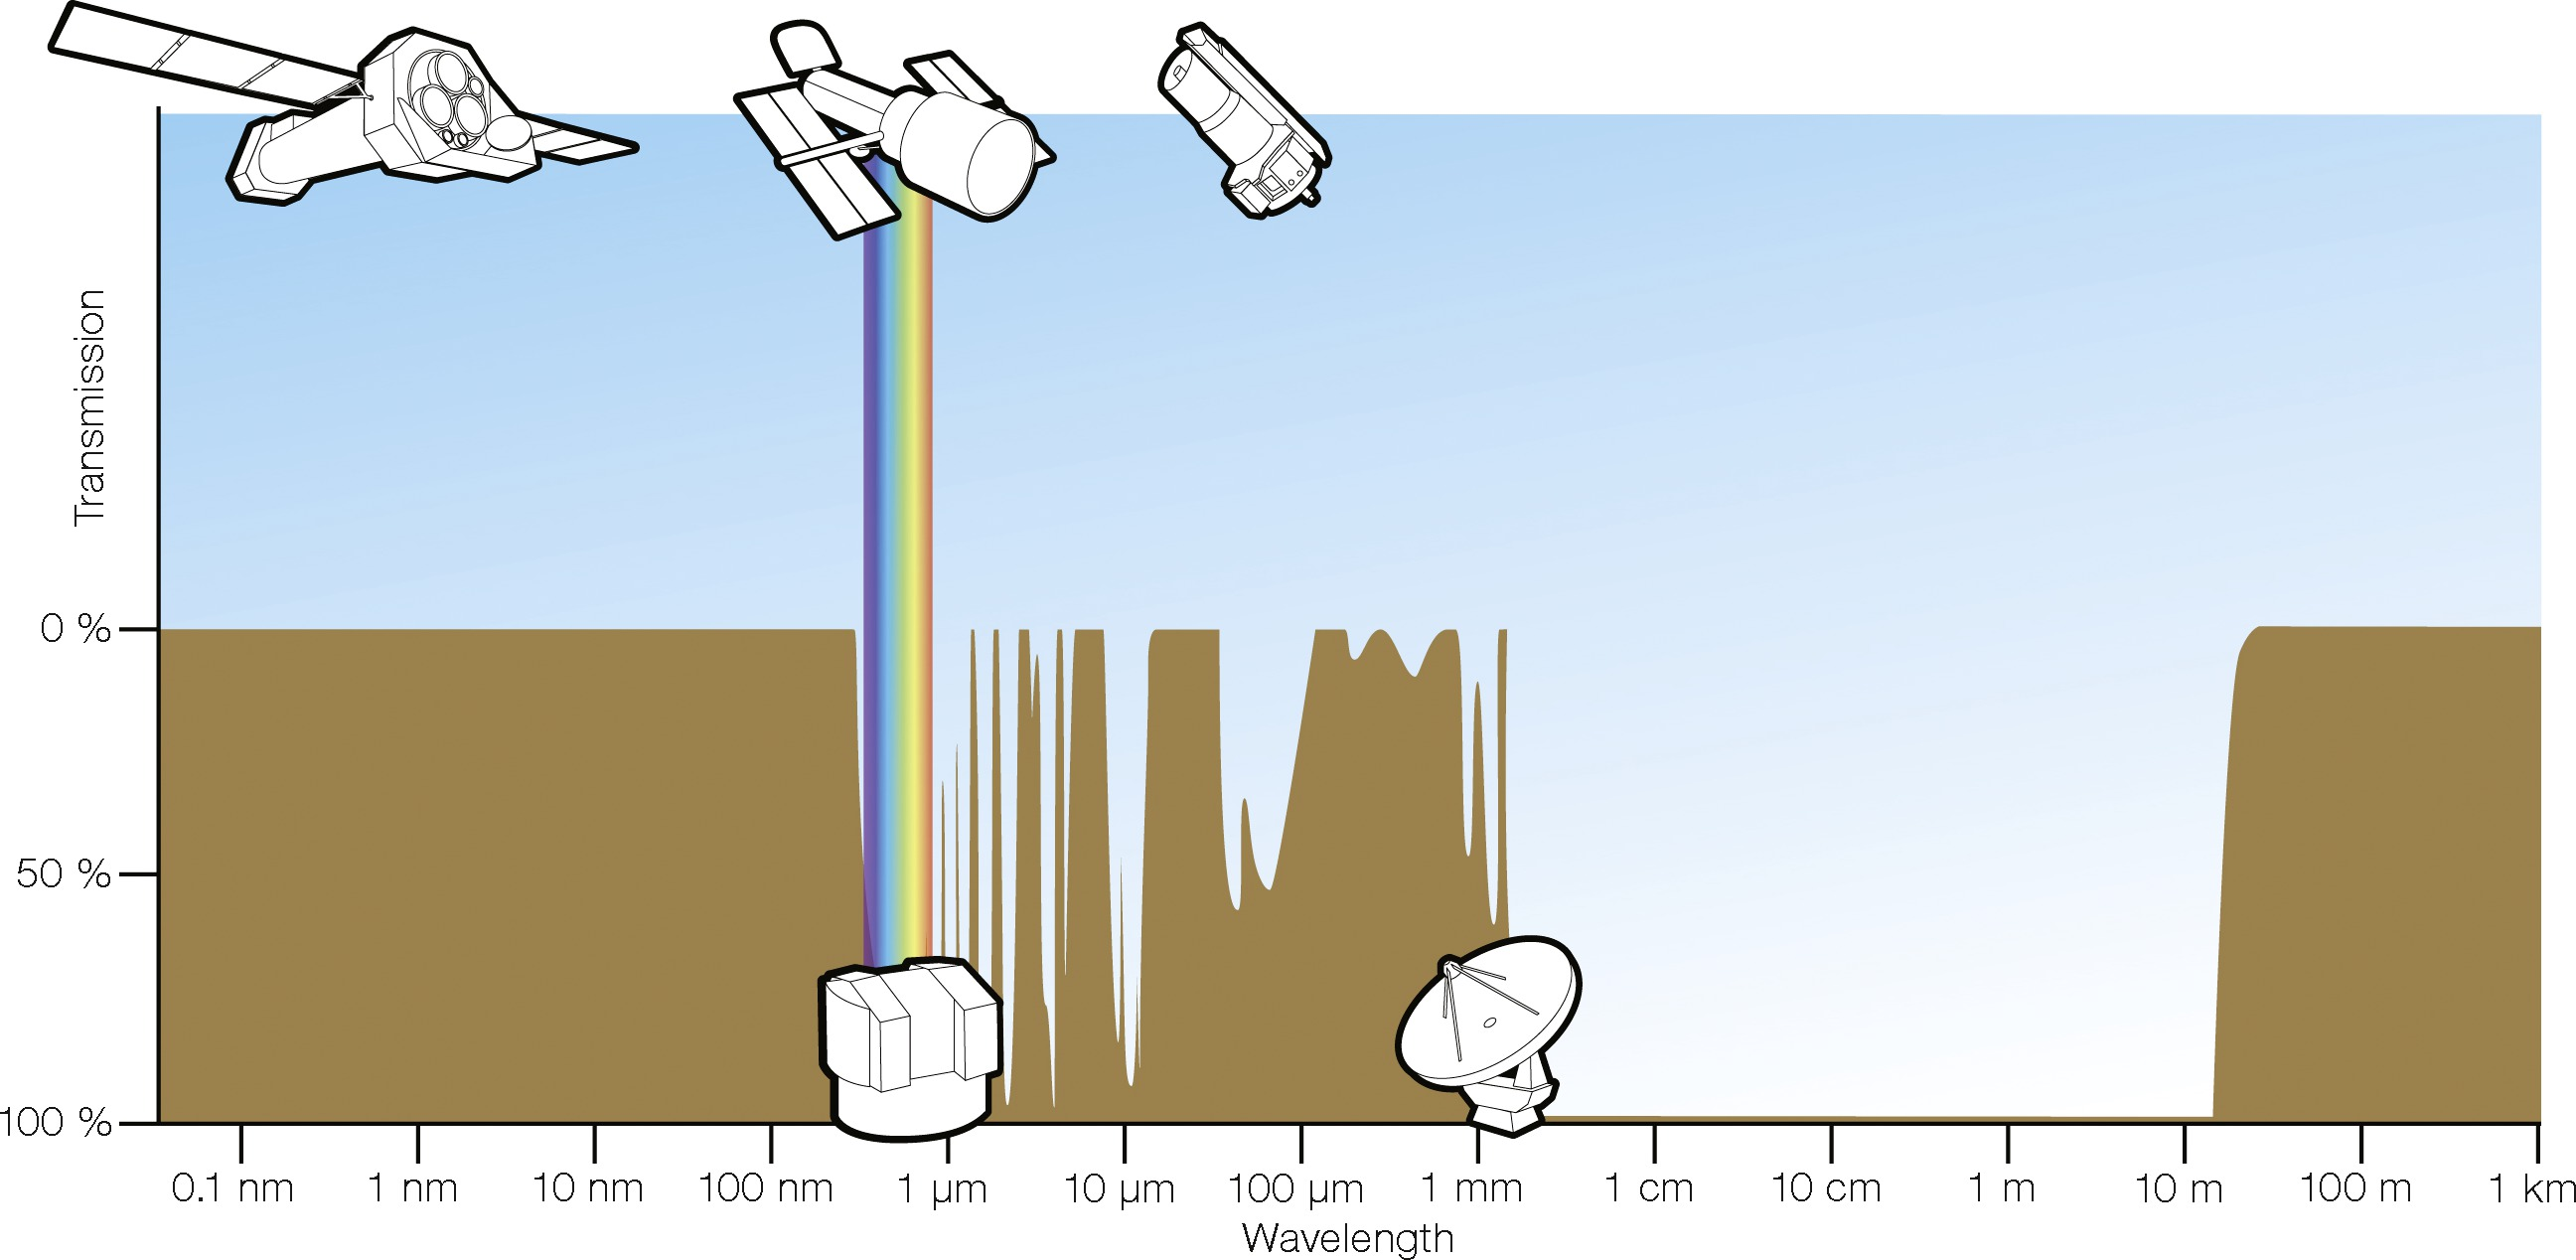
\includegraphics[width=\textwidth]{atmospheric-em-transmittance}
  \bicaption[大气层的电磁辐射透射率]{%
    大气层的电磁辐射透射率随波长(即频率)的变化.
    除了光学窗口,大气层还有一个更加宽广的射电窗口,
    从 $\lambda \sim \SI{0.3}{\mm}$ ($\nu \sim \SI{1000}{\GHz}$)
    延伸到 $\lambda \sim \SI{30}{\meter}$ ($\nu \sim \SI{10}{\MHz}$).
    大气层对电磁辐射的吸收情况会随时间以及地理位置而变化.
  }{%
    Electromagnetic transmittance of the Earth's atmosphere.
    In addition to the visible optical window, there is another
    much wider radio window, which spans from
    $\lambda \sim \SI{0.3}{\mm}$ ($\nu \sim \SI{1000}{\GHz}$)
    to $\lambda \sim \SI{30}{\meter}$ ($\nu \sim \SI{10}{\MHz}$).
    \\\textcopyright{}
    \citeay{condon2016}, \S\,1.1.2.
  }
  \label{fig:atmospheric-emt}
\end{figure}

首次发现源自地球之外的射电辐射是在 1932 年被 Bell 电话实验室的工程师
Karl Guthe Jansky 意外得到的.
上世纪 20 年代,Bell 电话公司基于短波($\lambda \sim \SI{15}{\meter}$)传输
建设了跨洋电话服务,但是发现通话受到了强烈的干扰,因此 Bell 电话实验室派
Jansky 去查明干扰来源.
Jansky 建造了一个对方向敏感的可转动天线(如\autoref{fig:jansky-antenna} 所示)
用来监测 \SI{20.5}{\MHz} ($\lambda \approx \SI{14.6}{\meter}$) 处的射电辐射.
经过观测,他发现绝大部分的干扰源自暴风雨的闪电.
此外,他还发现有一个较弱的不明噪声,其强度在每天发生周期性的变化,
他怀疑该噪声可能源自太阳的射电辐射.
但是持续的观测显示该不明噪声的准确周期为 \SI{23}{\hour}\,\SI{56}{\minute},
并不是刚好 \SI{24}{\hour}.
将此困惑与他的一个天文学家朋友 Albert Melvin Skellett 讨论后,
Jansky 了解到该噪声应来自太阳系之外,并进一步确认其来源是银河系中心 \cite{jansky1933}.

\begin{figure}[htp]
  \centering
  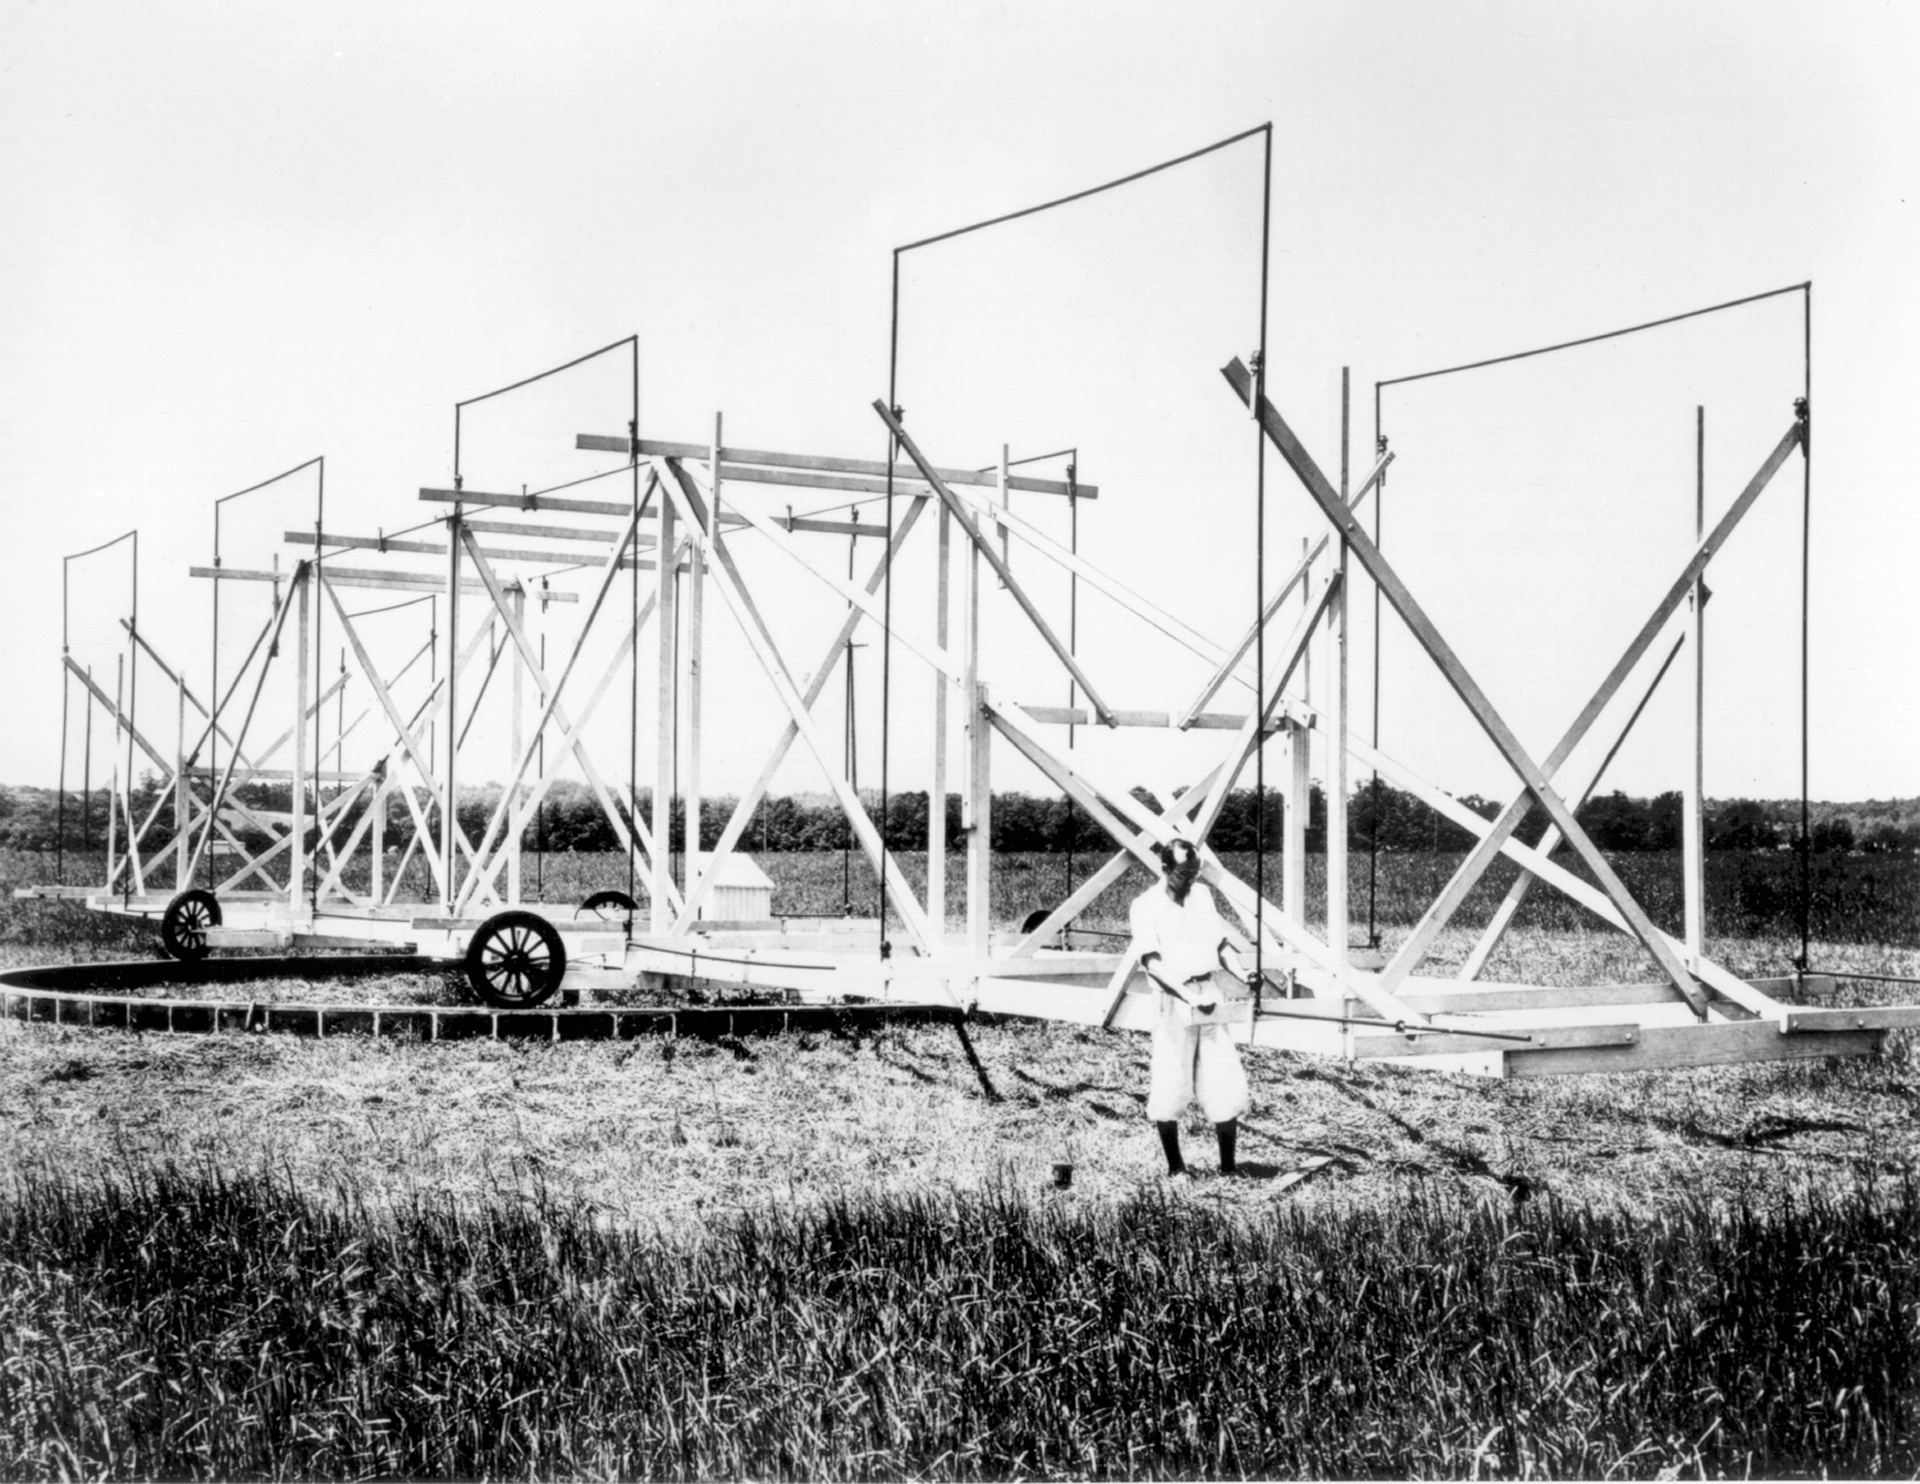
\includegraphics[width=0.8\textwidth]{KarlJansky-antenna}
  \bicaption[Karl G. Jansky 和他的天线]{%
    Karl G. Jansky 和他的天线.
    该天线可转动,主要接收水平方向的辐射.
  }{%
    Karl G. Jansky and the antenna that discovered the cosmic radio emission.
    The antenna can rotate in azimuth and mainly receive horizontal
    emissions.
    \\\textcopyright{}
    \ac{nrao}/\ac{aui}/\ac{nsf}.
  }
  \label{fig:jansky-antenna}
\end{figure}

然而,Jansky 的发现未能得到足够的关注和重视,他本人也被分配到其他项目而无法继续
详细研究银河系的射电辐射.
幸运的是,另一位无线电工程师 Grote Reber 对 Jansky 的发现产生了极大兴趣,
于是耗费数年在自家后院建造了世界第一台抛物面射电望远镜
(如\autoref{fig:reber-telescope} 所示).
在 1938 年,Reber 用这台望远镜成功地在 \SI{160}{\MHz} 探测到了银河系的辐射.
他进一步开展了银河系的第一次射电巡天观测,这些结果发表于专业的天文期刊
\apj \cite{reber1940},使得 Jansky 的成果得到了应有的重视.

\begin{figure}[htp]
  \centering
  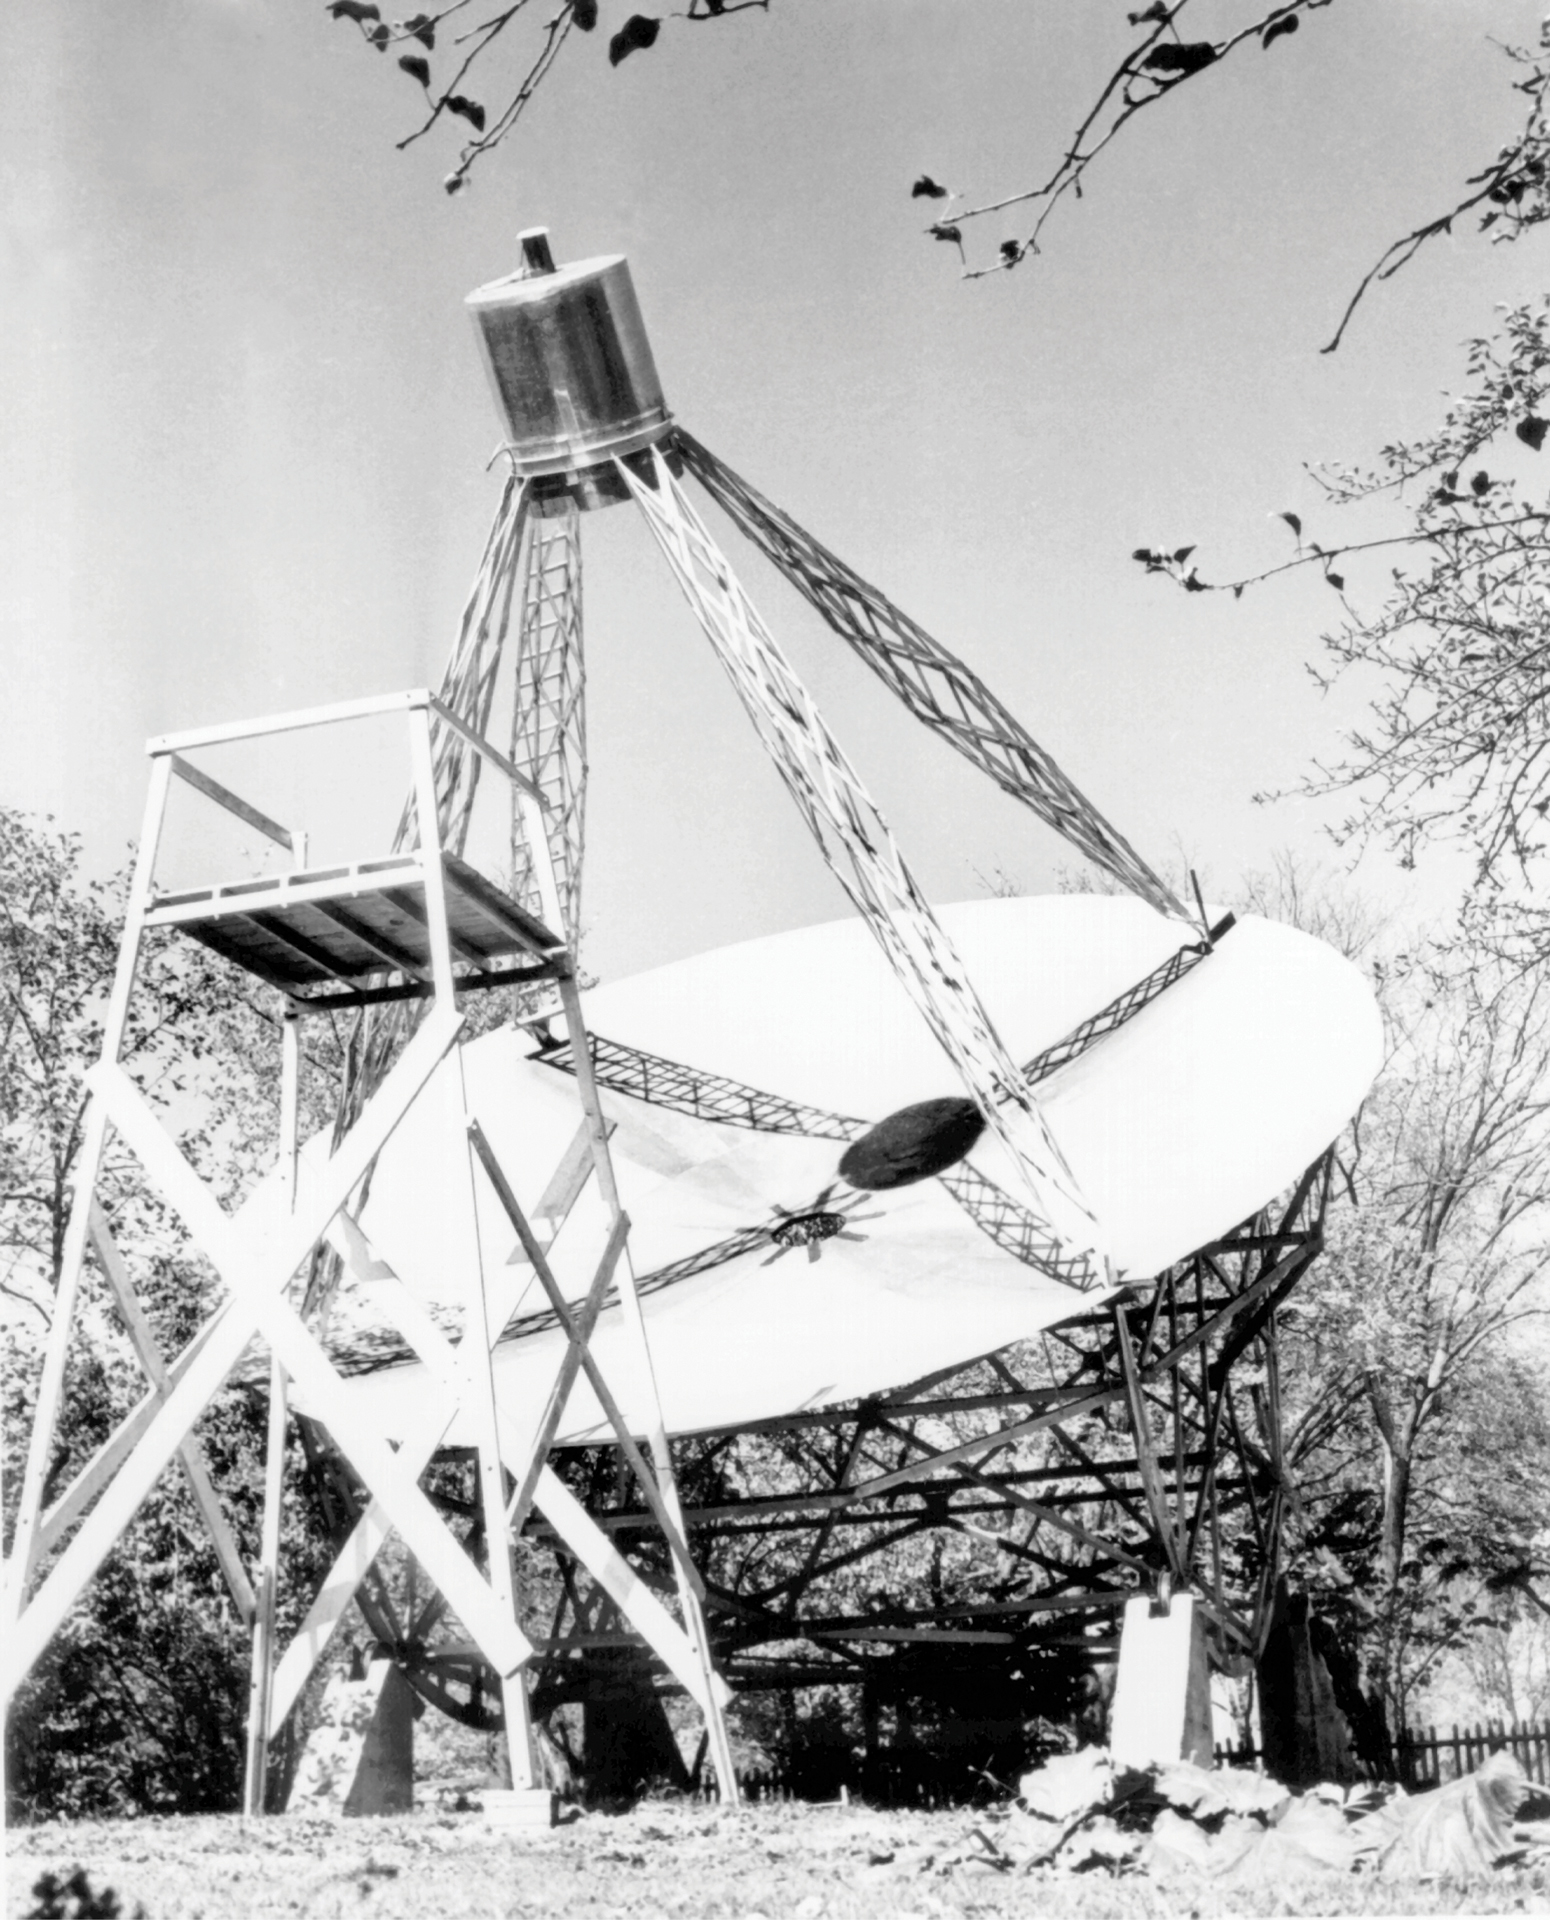
\includegraphics[width=0.6\textwidth]{GroteReber-telescope}
  \bicaption[Grote Reber 的射电望远镜]{%
    Grote Reber 在自家后院建造的射电望远镜,使用了直径约 \SI{10}{\meter} 的抛物面.
  }{%
    Grote Reber's backyard radio telescope using a parabolic reflector
    of diameter about \SI{10}{\meter}.
    \\\textcopyright{}
    \acs{nrao}/\acs{aui}/\acs{nsf}.
  }
  \label{fig:reber-telescope}
\end{figure}

后续的几年里,尽管第二次世界大战阻碍了射电天文的发展,但是极大地刺激了无线电技术
和雷达设备的研发.
这些方面的成果在战争结束后给射电天文学带来了长足进步,开创了一系列新技术和新方法.
其中最值得一提的是由 Martin Ryle 和 Antony Hewish 发明的\ac{as}技术,
使射电观测的角分辨率和灵敏度得到了空前的提高.

自射电窗口被打开以来,射电天文学已取得了一系列激动人心的新发现,主要包括:
银河系和其他多种天体的非热辐射 \cite{reber1940}、
由超大质量黑洞驱动的射电星系\cite{baade1954}和\ac{quasar}\cite{hazard1963,schmidt1963}及其演化、
冷星际介质(如原子、离子和分子)的热辐射谱线、
星际分子的\ac{maser} \cite{weaver1965}、
源自宇宙大爆炸的 \ac{cmb} \cite{penzias1965}、
\ac{pulsar}和中子星 \cite{hewish1968}、
星系的 \ac{hi} 旋转曲线显示其内部存在\ac{dm} \cite{roberts1975}、
强\ac{gl} \cite{walsh1979}.
总之,射电天文学揭开了宇宙在光学波段所见完全不同的一面(如\autoref{fig:radio-sky} 所示),
极大地拓展了我们对宇宙的认识,深刻地改变了我们对宇宙的理解.

\begin{figure}[htp]
  \centering
  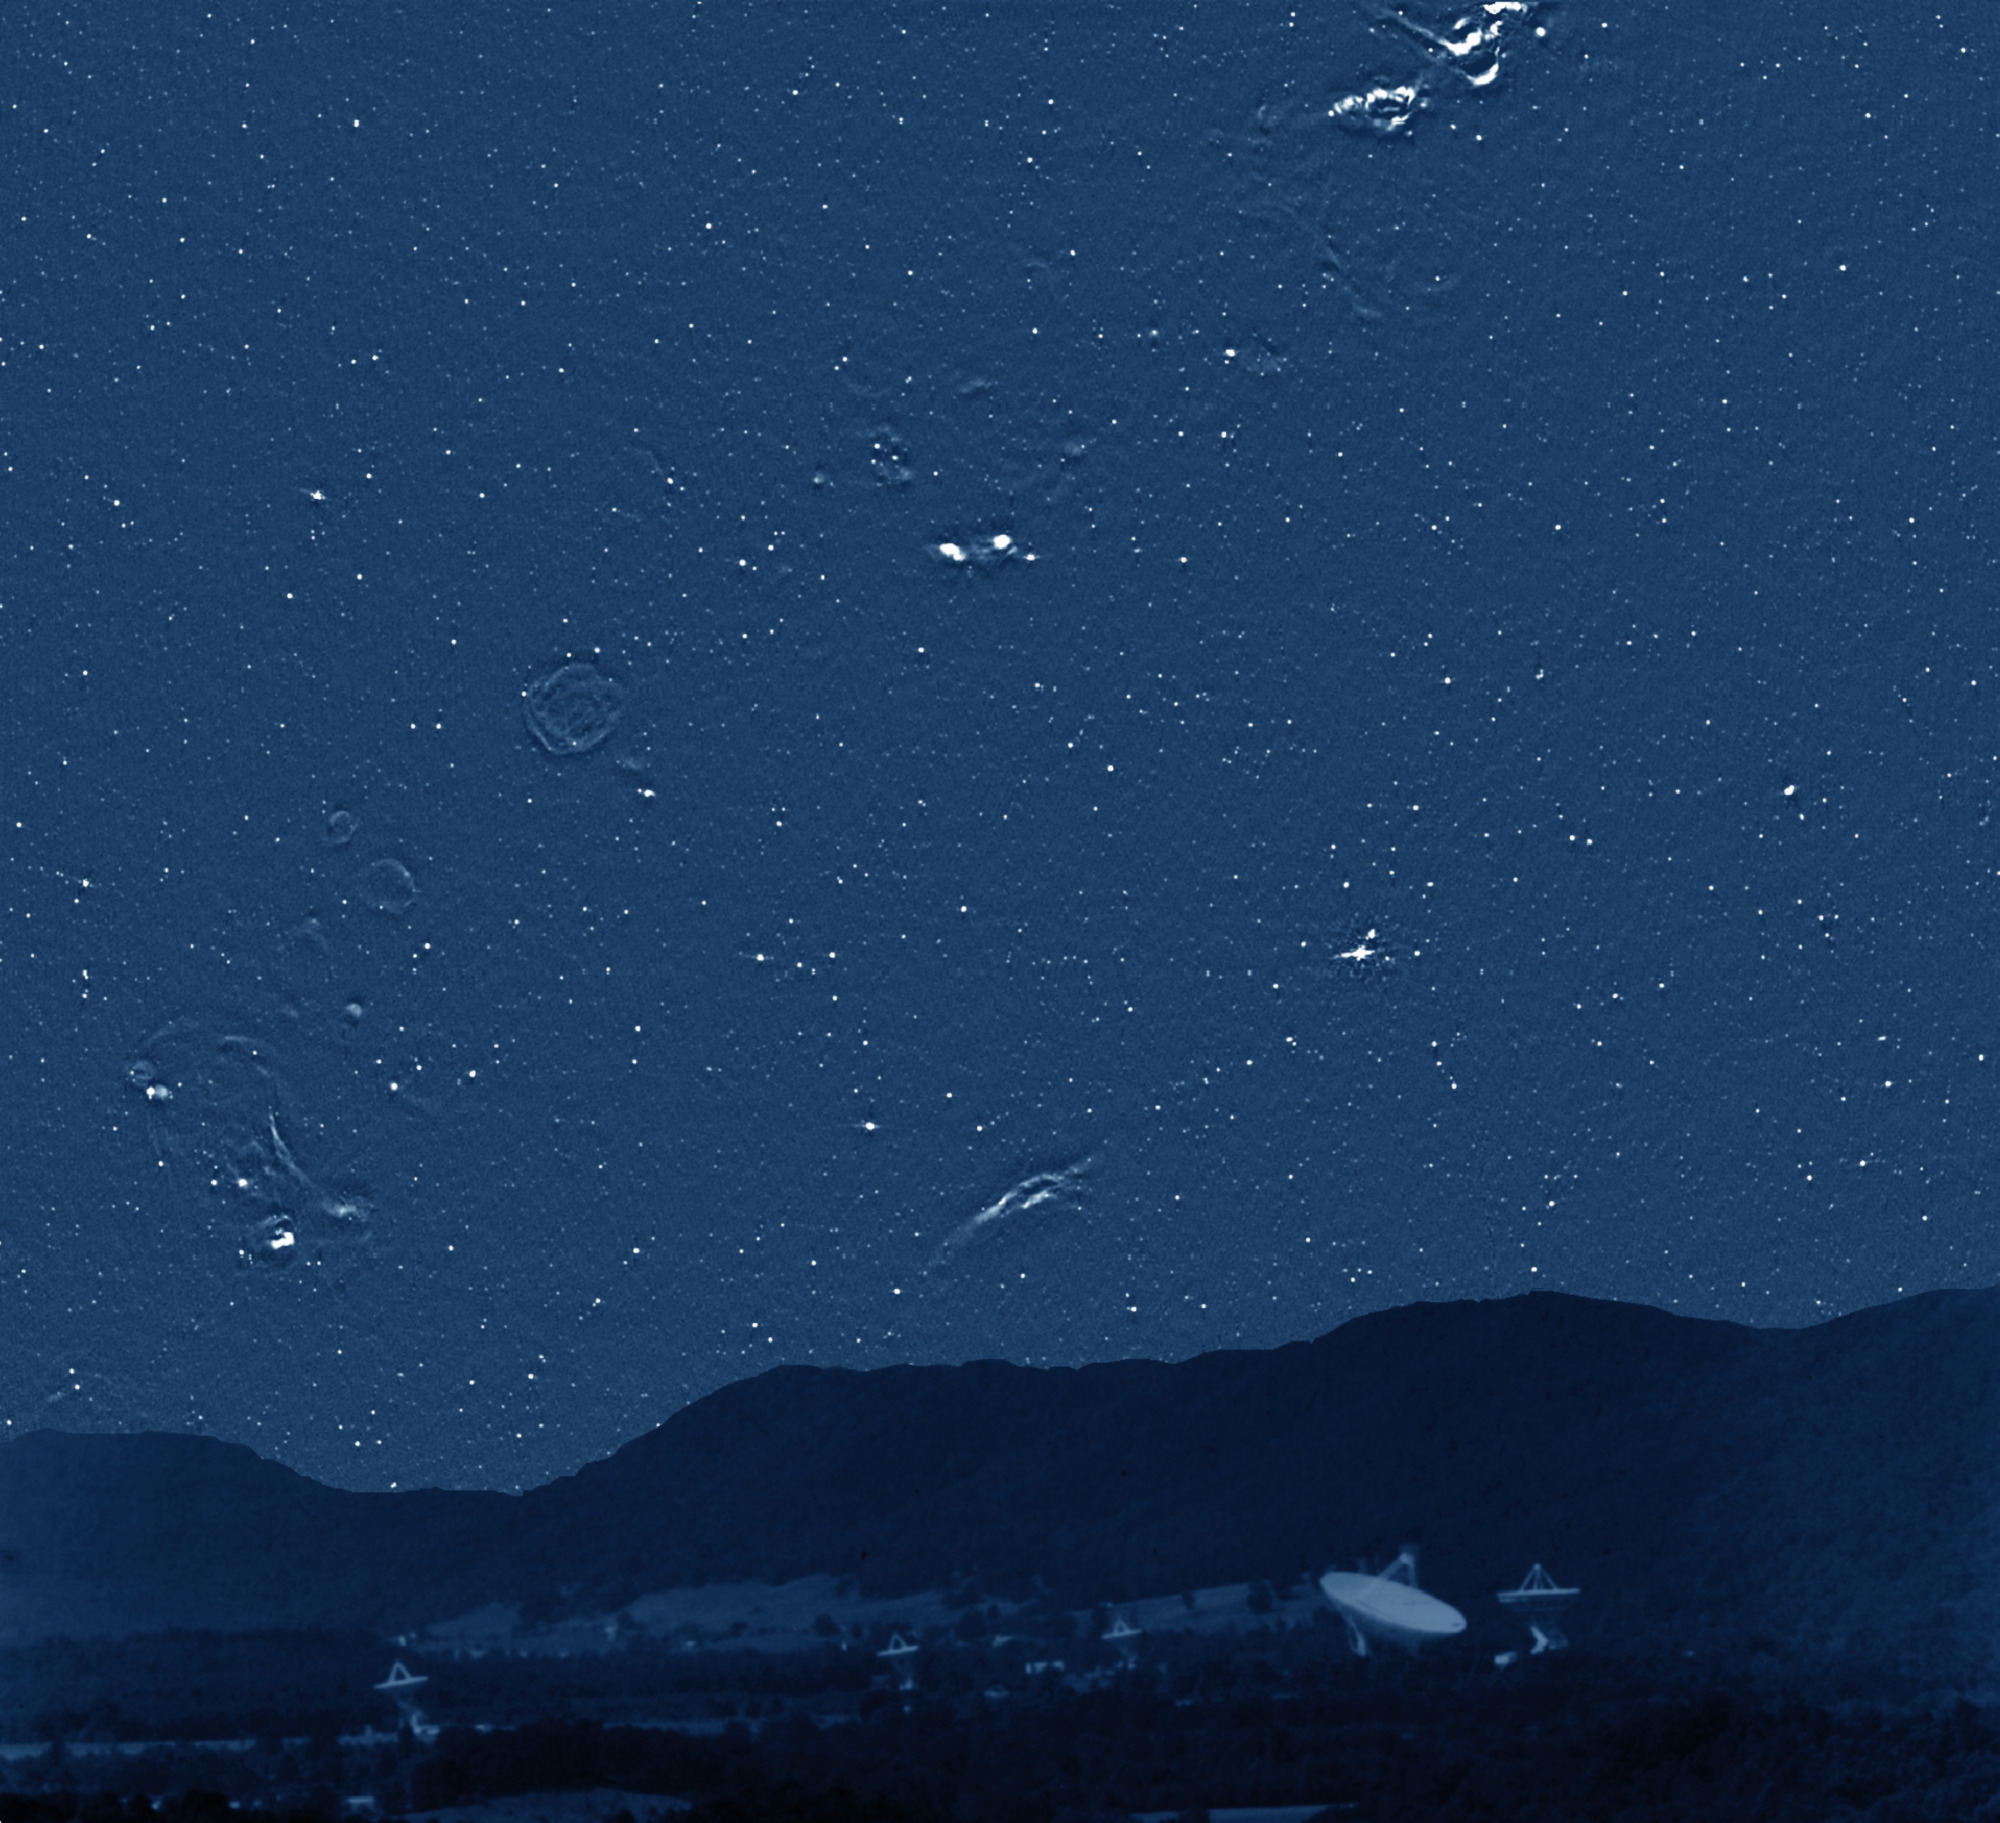
\includegraphics[width=0.8\textwidth]{nrao-radio-sky}
  \bicaption[与光学波段所见完全不同的射电天空]{%
    在 NRAO 台址的照片上方显示了由 NRAO 前 \SI{91}{\meter} 射电望远镜获得的
    \SI{4.85}{\GHz} 射电天空图像.
  }{%
    The \SI{4.85}{\GHz} radio sky made with the NRAO former \SI{91}{\meter}
    telescope is shown above an old photograph of the NRAO site.
    \\\textcopyright{}
    \acs{nrao}/\acs{aui}/\acs{nsf}.
  }
  \label{fig:radio-sky}
\end{figure}

%---------------------------------------------------------------------
\subsection{机遇和挑战}

尽管大气层的射电窗口允许低至约 \SI{10}{\MHz} 的观测,但由于各种技术和条件的限制,
以往的射电观测和研究主要位于 $\gtrsim \si{\GHz}$ 的中高频波段.
相比中高频波段,低频波段(约 \SIrange{50}{300}{\MHz})主要有以下几点优势:
\begin{itemize}
  \item 低频波段对应的辐射波长更长,受尘埃的影响更小,因此能够观测到星系更核心的区域.
  \item \ac{rad-syn}在低频波段更强且寿命更长,因此更利于探测\ac{gc}、
    \ac{sc}甚至\ac{lsf}的弥散射电辐射.
  \item 多种等离子体效应(如散射、色散、Faraday 旋转)的强度按 $\nu^{-2}$ 变化,
    因此在低频波段更适合研究星际电子密度、磁场强度、等等.
  \item 源自宇宙再电离时期 (红移 $z \sim \numrange{6}{16}$)
    的\ac{hi} 21\,cm 信号历经红移后将出现在低频波段,因此不可避免地需要在
    此波段开展观测,探测该信号以研究宇宙早期的再电离过程
    (详见 \autoref{sec:eor-signal}).
  \item 低频射电望远镜通常具有大视场,能够显著提高巡天速度,非常有利于搜寻
    脉冲星、暂现源、等等.
\end{itemize}

随着相关技术取得了充分发展,低频射电波段已在近十多年来得到了重点关注并取得了长足进步,
目前已建成一批工作在此波段的干涉阵列,
主要包括 \ac{21cma}、\ac{gmrt}、\ac{mwa}、\ac{lofar}.
此外还有若干正在积极建设的新型低频干涉阵列,比如 \ac{lwa}、\ac{hera}、\ac{ska}.
可见,低频射电波段正在成为射电天文及至整个天文领域的热点和前沿,

当然,在低频波段开展观测也面临更大的挑战,
比如强烈的人工源\ac{rfi}、\ac{ionosphere}的扰动、
通常需要建设更大更复杂的干涉阵列、解决更复杂的仪器效应、
研发更有效的数据处理方法(参见 \autoref{sec:det-difficulties}).
尽管如此,可以肯定低频射电天文将成为射电天文领域的重要力量,
并为整个天文学的发展作出不可磨灭的贡献.


%=====================================================================
\section{辐射基础}
\label{sec:radiation}

%---------------------------------------------------------------------
\subsection{基本概念}

\begin{figure}[htp]
  \centering
  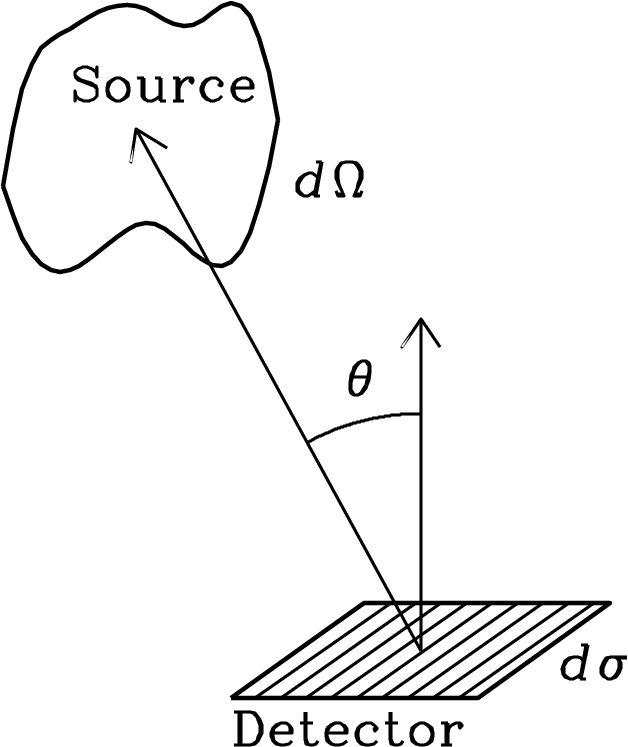
\includegraphics[width=0.3\textwidth]{specific-intensity}
  \bicaption[\acl*{I-nu} \acs*{I-nu} 的测量]{%
    \acl*{I-nu} \acs*{I-nu} 的测量示意图.
  }{%
    The specific intensity \acs*{I-nu} measured by a detector of area
    $\D{\sigma}$ to a source extending a solid angle of $\D{\Omega}$.
    \\\textcopyright{}
    \citeay{condon2016}, \S\,2.1.
  }
  \label{fig:intensity}
\end{figure}

考虑一个面积为 $\D{\sigma}$ 的探测器,测量一个与其法线方向呈 $\theta$ 角度、
所张立体角为 $\D{\Omega}$ 的源的辐射(如\autoref{fig:intensity} 所示),
若探测器在频率范围 $[\nu, \,\nu+\D{\nu}]$ 内接收到的功率为 $\D{P_{\nu}}$,
则源的\emph{\acf{I-nu}} 为:
\begin{equation}
  \label{eq:intensity}
  \acs{I-nu} \equiv
    \frac{\D{P_{\nu}}}{(\cos\theta\,\D{\sigma}) \,\D{\nu} \,\D{\Omega}} \,,
\end{equation}
其 \ac{si} 单位是 [\si{\watt\per\square\meter\per\hertz\per\steradian}].
\acl{I-nu} \acs{I-nu} 亦被称为\emph{谱亮度 (spectral brightness)},
有时也被简称为\emph{强度}或\emph{亮度}.

\begin{figure}[htp]
  \centering
  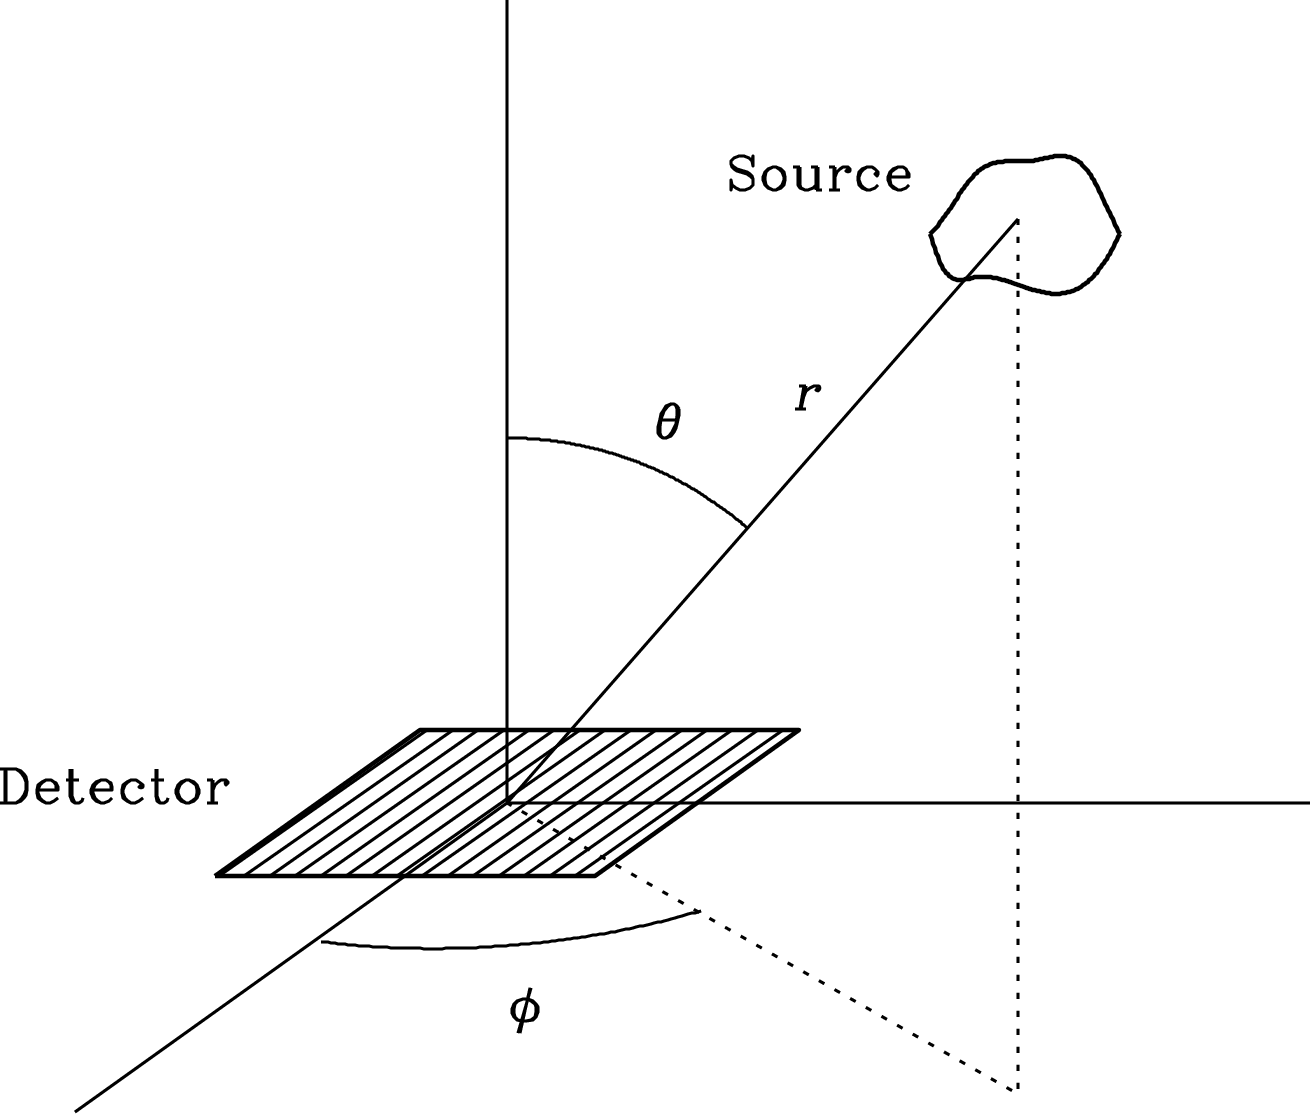
\includegraphics[width=0.5\textwidth]{flux-density}
  \bicaption[\acl*{S-nu} \acs*{S-nu} 的定义示意图]{%
    \acl*{S-nu} \acs*{S-nu} 的定义示意图.
  }{%
    An illustration of the definition of flux density \acs*{S-nu}.
    \\\textcopyright{}
    \citeay{condon2016}, \S\,2.1.
  }
  \label{fig:flux-density}
\end{figure}

对于一个离散源,其所张的立体角是确定的,如图\autoref{fig:flux-density} 所示,
因此探测器单位投影面积上接收到的谱功率 (spectral power)
即为这个源的\emph{\acf{S-nu}}:
\begin{equation}
  \label{eq:flux-density}
  \acs{S-nu} \equiv
    \int_{\R{source}} \acs{I-nu}(\theta,\phi) \cos\theta \,\D{\Omega} ,
\end{equation}
其 \ac{si} 单位是 [\si{\watt\per\square\meter\per\hertz}].
实际中常用的单位是 \si{\jansky},换算关系为
$\SI{1}{\jansky} = \SI{e-26}{\watt\per\square\meter\per\hertz}$.

辐射场的\emph{\acf{u-nu}}是指每单位体积的谱能量 (spectral energy)
其 \ac{si} 单位为 [\si{\joule\per\cubic\meter\per\hertz}].
取辐射场中的一个体积元 $\D{V}$,对于来自某一方向的立体角元 $\D{\Omega}$
的一束辐射 $\acs{I-nu}(\theta,\phi)$,
可认为体积元 $\D{V}$ 具有长度 $\D{s}$ 以及横截面积 $\D{\sigma}$,
即 $\D{V} = \D{s}\,\D{\sigma}$,
于是这束辐射 $\acs{I-nu}(\theta,\phi)$ 对该体积元的谱能量贡献为:
\begin{equation}
  \D{\acs{u-nu}}\,\D{V}
    = \acs{I-nu}(\theta,\phi) \,\D{\Omega}\,\D{\sigma}
      \left( \frac{\D{s}}{\acs{speed-light}} \right) ,
\end{equation}
其中 \acs{speed-light} 是\acl{speed-light}.
将上式对所有方向积分,即得辐射场的\acl{u-nu}:
\begin{equation}
  \label{eq:spectral-energy-density}
  \acs{u-nu}
    = \int_{4\Cpi} \D{\acs{u-nu}}
    = \frac{1}{\acs{speed-light}}
      \int_{4\Cpi} \acs{I-nu}(\theta,\phi) \,\D{\Omega} .
\end{equation}
如果辐射场是各向同性的,即 $\acs{I-nu}(\theta,\phi) = \acs{I-nu}$,则有:
\begin{equation}
  \label{eq:spectral-energy-density-iso}
  \acs{u-nu} = \frac{4\Cpi \, \acs{I-nu}}{\acs{speed-light}} .
\end{equation}

%---------------------------------------------------------------------
\subsection{辐射转移}
\label{sec:radiative-transfer}

\begin{figure}[htp]
  \centering
  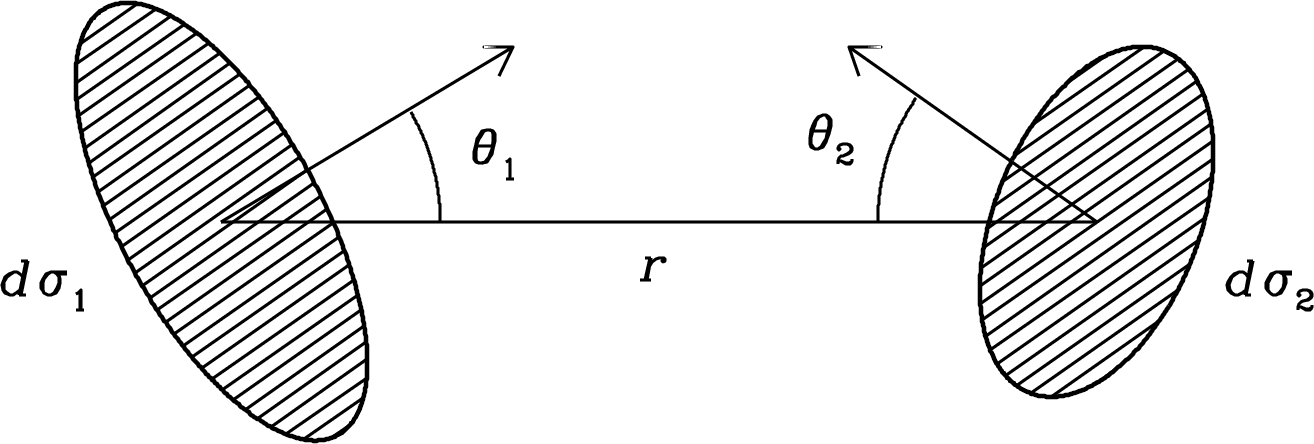
\includegraphics[width=0.6\textwidth]{specific-intensity-conservation}
  \bicaption[\acl*{I-nu} \acs*{I-nu} 沿光线保持不变]{%
    在自由空间里\acl*{I-nu} \acs*{I-nu} 沿光线保持不变.
  }{%
    The specific intensity \acs*{I-nu} conserved along a ray in empty space.
    \\\textcopyright{}
    \citeay{condon2016}, \S\,2.1.
  }
  \label{fig:intensity-conservation}
\end{figure}

在自由空间里,即不存在吸收和发射,辐射的\acl*{I-nu} \acs*{I-nu} 保持不变,与距离无关.
考虑由源发射的一束光线,
设 $\D{\sigma_1}$ 和 $\D{\sigma_2}$ 是光线上相距为 $r$ 的两个无限小截面,
如\autoref{fig:intensity-conservation} 所示,
则两个面元相互所张的立体角为:
\begin{align}
  \D{\Omega_1} & = \frac{\cos\theta_2 \,\D{\sigma_2}}{r^2} , \\
  \D{\Omega_2} & = \frac{\cos\theta_1 \,\D{\sigma_1}}{r^2} .
\end{align}
于是,在频率范围 $[\nu, \,\nu+\D{\nu}]$ 以及立体角 $\D{\Omega_1}$ 之内
流过面元 $\D{\sigma_1}$ 的功率为:
\begin{align}
  \D{P_1} & = (\acs{I-nu})_1 \cos\theta_1
      \,\D{\Omega_1} \,\D{\sigma_1} \,\D{\nu}  \\
    & = (\acs{I-nu})_1 \left( \frac{\cos\theta_1 \cos\theta_2}{r^2} \right)
      \,\D{\sigma_1} \,\D{\sigma_2} \,\D{\nu} ,
\end{align}
类似地,流过面元 $\D{\sigma_2}$ 的功率为:
\begin{align}
  \D{P_2} & = (\acs{I-nu})_2 \cos\theta_2
      \,\D{\Omega_2} \,\D{\sigma_2} \,\D{\nu}  \\
    & = (\acs{I-nu})_2 \left( \frac{\cos\theta_1 \cos\theta_2}{r^2} \right)
      \,\D{\sigma_1} \,\D{\sigma_2} \,\D{\nu} .
\end{align}
利用能量守恒,即 $\D{P_1}\,\D{t} = \D{P_2}\,\D{t}$,
可得:
\begin{equation}
  \label{eq:intensity-conservation}
  (\acs{I-nu})_1 = (\acs{I-nu})_2 .
\end{equation}

\begin{figure}[htp]
  \centering
  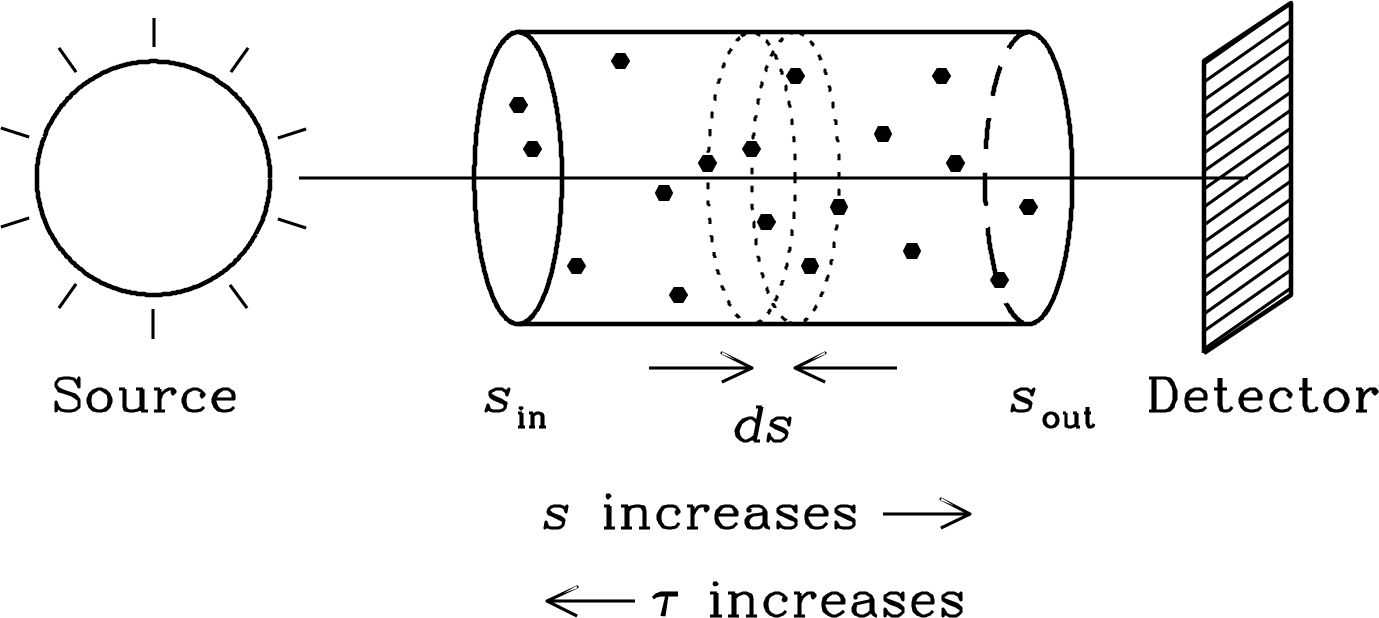
\includegraphics[width=0.6\textwidth]{radiative-transfer}
  \bicaption[辐射转移示意图]{%
    辐射转移示意图.
    距离 $s$ 沿源向探测器的方向增长,介质的入端和出端的距离分别为
    $s_{\R{in}}$ 和 $s_{\R{out}}$.
    光深 $\tau$ 的增长方向与 $s$ 相反.
  }{%
    An illustration of the radiative transfer.
    The distance $s$ increases along the ray from the source to the detector.
    The distances at the input end and the output end of the intervening
    medium are $s_{\R{in}}$ and $s_{\R{out}}$, respectively.
    The optical depth $\tau$ is measured in the opposite direction as $s$.
    \\\textcopyright{}
    \citeay{condon2016}, \S\,2.2.
  }
  \label{fig:radiative-transfer}
\end{figure}

当传播空间中存在吸收和发射时(如\autoref{fig:radiative-transfer} 所示),
辐射的\acl{I-nu} \acs{I-nu} 会发生改变,具体变化可由\emph{\acf{rt}}方程描述.
首先考虑吸收情形,一个辐射光子通过介质中一个厚度为 $\D{s}$ 的薄层时被吸收的概率 $\D{p}$ 为:
\begin{equation}
  \D{p} = \acs{coef-absorption} \,\D{s} ,
\end{equation}
其中 \acs{coef-absorption} 为\emph{\acl{coef-absorption}},
量纲为 $\big[\text{长度}^{-1}\big]$.
于是,\acl{I-nu} \acs{I-nu} 在通过厚度 $\D{s}$ 的介质后的损失比例为:
\begin{equation}
  \label{eq:rt-absorption}
  \frac{\D{\acs{I-nu}}}{\acs{I-nu}} = - \acs{coef-absorption} \,\D{s} .
\end{equation}
对上式的两边沿介质的吸收路径积分,可得:
\begin{equation}
  \int_{s_{\R{in}}}^{s_{\R{out}}} \frac{\D{\acs{I-nu}}}{\acs{I-nu}}
    = \ln\acs{I-nu} \,\Big|_{s_{\R{in}}}^{s_{\R{out}}}
    = - \int_{s_{\R{in}}}^{s_{\R{out}}} \acs{coef-absorption}(s') \,\D{s'} ,
\end{equation}
即
\begin{equation}
  \label{eq:intensity-loss1}
  \frac{\acs{I-nu}(s_{\R{out}})}{\acs{I-nu}(s_{\R{in}})} =
    \exp \left[ - \int_{s_{\R{in}}}^{s_{\R{out}}}
      \acs{coef-absorption}(s') \,\D{s'} \right] .
\end{equation}
据此,可定义\emph{\acf{optical-depth}}为:
\begin{equation}
  \label{eq:optical-depth}
  \acs{optical-depth} \equiv
    - \int_{s_{\R{out}}}^{s_{\R{in}}} \acs{coef-absorption}(s') \,\D{s'} .
\end{equation}
注意,上式的积分方向与 $s$ 相反(另见\autoref{fig:radiative-transfer}),
如此可使 $\tau > 0$ 并且随着观测者对介质的观测深度而增大.
利用\acl{optical-depth} \acs{optical-depth},
\autoref{eq:intensity-loss1} 可以写成:
\begin{equation}
  \label{eq:intensity-loss}
  \frac{\acs{I-nu}(s_{\R{out}})}{\acs{I-nu}(s_{\R{in}})} =
    \exp (-\acs{optical-depth}) .
\end{equation}
当 $\tau \ll 1$ 时,称介质是\emph{光学薄}的;
当 $\tau \gg 1$ 时,则称介质是\emph{光学厚}的.

另一方面,介质可能产生辐射使\acl{I-nu} \acs{I-nu} 增强.
考虑介质中的一个体积元 $\D{s}\,\D{\sigma}$,在频率范围 $[\nu, \,\nu+\D{\nu}]$ 内
沿某一方向的立体角元 $\D{\Omega}$ 所发射的谱功率为:
\begin{equation}
  \D{P_{\nu}} =
    \acs{coef-emission} \,\D{s}\,\D{\sigma}\,\D{\nu}\,\D{\Omega} ,
\end{equation}
其中 \acs{coef-emission} 为\emph{\acl{coef-emission} (emission coefficient)}.
当不存在吸收时,\acs{coef-emission} 可表示为:
\begin{equation}
  \label{eq:coef-emission}
  \acs{coef-emission} = \diff{\acs{I-nu}}{s} .
\end{equation}
易知 \acs{coef-emission} 的单位为
[\si{\watt\per\cubic\meter\per\hertz\per\steradian}].
综合上式和\autoref{eq:rt-absorption},可得\emph{\ac{rt}方程}:
\begin{equation}
  \label{eq:radiative-transfer}
  \diff{\acs{I-nu}}{s} =
    - \acs{coef-absorption} \,\acs{I-nu} + \acs{coef-emission} .
\end{equation}

%---------------------------------------------------------------------
\subsection{Kirchhoff 定律}

\emph{\acf{te}},简称\emph{热平衡},
是指一个系统在没有外界影响的条件下,其各部分的宏观属性在长时间内不发生任何变化的状态.
这是热力学中的一个基本实验定律,是定义温度的基础.

\begin{figure}[htp]
  \centering
  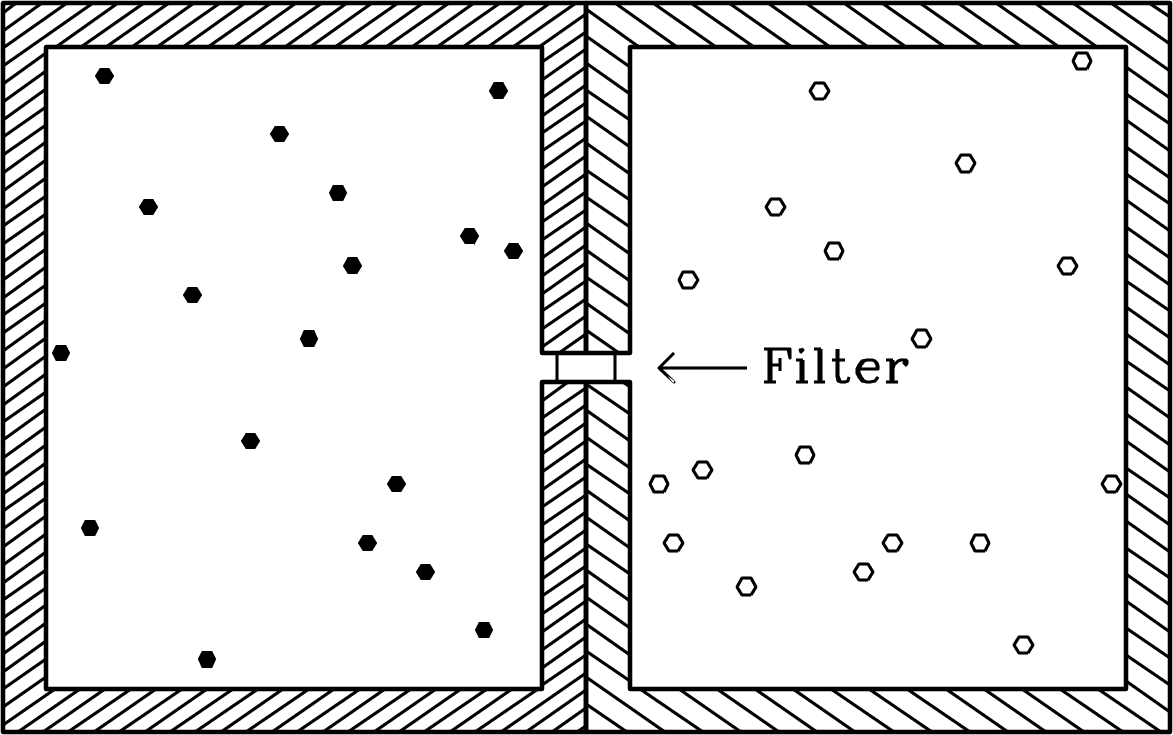
\includegraphics[width=0.5\textwidth]{Kirchhoff-law-experiment}
  \bicaption[推导 Kirchhoff 定律的思想实验]{%
    推导 Kirchhoff 定律的思想实验.
  }{%
    A thought experiment to derive the Kirchhoff's law.
    \\\textcopyright{}
    \citeay{condon2016}, \S\,2.2.
  }
  \label{fig:kirchhoff-experiment}
\end{figure}

考虑如下思想实验:
两个由不同材料制成、包含不同介质的空腔放在一起,
中间由一个仅允许频率在 $[\nu, \,\nu+\D{\nu}]$ 之间的辐射通过的阀门连接,
如\autoref{fig:kirchhoff-experiment} 所示.
在\emph{完全热平衡}的情形下,即物质和辐射场具有相同的温度,
空腔产生的辐射与黑体辐射(见 \autoref{sec:blackbody})相同,
完全由温度决定,而与其材质或者内部介质无关.
当两个空腔在任意温度 $T$ 达到完全热平衡时,没有\emph{净}能量从一个空腔辐射到另一个,
否则损失能量的空腔将冷却,另一个空腔将升温,从而违背热力学第二定律.
由此可知:
\begin{align}
  \diff{\acs{I-nu}}{s} & = 0 , \\
  \acs{I-nu} & = B_{\nu}(T) ,
\end{align}
其中 $B_{\nu}(T)$ 为空腔的辐射频谱.
于是辐射转移方程 [\autoref{eq:radiative-transfer}] 成为:
\begin{equation}
  \diff{\acs{I-nu}}{s} = 0
    = - \acs{coef-absorption} \,B_{\nu}(T) + \acs{coef-emission} ,
\end{equation}
所以:
\begin{equation}
  \label{eq:kirchhoff-law}
  \frac{\acs{coef-emission}(T)}{\acs{coef-absorption}(T)} = B_{\nu}(T) ,
\end{equation}
该式对任意频率 $\nu$ 均成立.
这就是完全热平衡系统的\emph{Kirchhoff 定律}.

完全的热平衡只有在特殊的条件下才能实现.
对于一般的系统,产生发射或吸收的物质并不与辐射场达到热平衡,但如果物质本身是热平衡的,
则称该系统处于\emph{\acf{lte}}.
Kirchhoff 定律 [\autoref{eq:kirchhoff-law}] 对此类系统同样适用,
不过 $\acs{I-nu}$ 与 $B_{\nu}(T)$ 通常不相等.

%---------------------------------------------------------------------
\subsection{黑体辐射和亮温度}
\label{sec:blackbody}

\emph{黑体}是能够吸收全部入射辐射的理想物体.
处于热力学平衡态的黑体产生的辐射称为\emph{黑体辐射},其能谱分布只取决于黑体的温度,
由 \emph{Planck 辐射定律}给出:
\begin{equation}
  \label{eq:planck}
  B_{\nu}(\nu, T) = \frac{2 h \nu^3}{\acs{speed-light}^2}
    \left[ \exp\left( \frac{h \nu}{\acs{kb} T} \right) - 1 \right]^{-1} ,
\end{equation}
其中 $B_{\nu}$ 是在频率 $\nu$ 处的谱亮度,$h$ 是 Planck 常数,
\acs{speed-light} 是\acl{speed-light}.

在射电波段,$h\nu \ll \acs{kb}T$ 通常成立,因此上式可近似为:
\begin{equation}
  \label{eq:rj-approx}
  B_{\nu}(\nu, T) \approx \frac{2\,\acs{kb}T \nu^2}{\acs{speed-light}^2} .
\end{equation}
该式就是 \emph{Rayleigh--Jeans 近似}.
在该近似下,辐射黑体的谱亮度 $B_{\nu}$ 与其温度 $T$ 严格成正比.
因此,一个源的谱亮度(即比强度) $I_{\nu}$
可以很方便地使用\emph{\acf{T-brightness}} 来描述:
\begin{equation}
  \label{eq:Tb}
  \acs{T-brightness}(\nu)
    \equiv \frac{\acs{I-nu} \acs{speed-light}^2}{2 \,\acs{kb} \nu^2} .
\end{equation}
注意 \acs{T-brightness} 会随频率而变.

%---------------------------------------------------------------------
\subsection{电阻的热噪声}

一个温度为 $T$ 的电阻 (resistor),因其内部的载流子(通常是电子)的随机热运动而产生噪声,
该噪声亦称 \emph{Johnson--Nyquist 噪声} \cite{johnson1928,nyquist1928},
其谱功率 (spectral power, 即每单位频率的功率) 由以下 \emph{Nyquist 近似}给出
[详见 \citeay{condon2016}, \S\,2.5]:
\begin{equation}
  \label{eq:nyquist-approx}
  P_{\nu} \approx \acs{kb} T .
\end{equation}
该式是 Rayleigh--Jeans 近似 [\autoref{eq:rj-approx}] 在电学里的对应.
类似地,该近似公式只适用于 $h\nu \ll \acs{kb}T$ 的经典范畴.
在考虑量子化修正后,严格的 \emph{Nyquist 公式}为:
\begin{equation}
  \label{eq:nyquist}
  P_{\nu} = h \nu
    \left[ \exp\left( \frac{h \nu}{\acs{kb} T} \right) - 1 \right]^{-1} .
\end{equation}


%=====================================================================
\section{谱线基础}
\label{sec:spectral-line}

\emph{\acf{spec-line}}是光谱上的窄($\Delta\nu \ll \nu$)发射或吸收特征,
均源自原子或分子的能级跃迁.
当一个原子或分子从高能级 $E_2$ 跃迁至低能级 $E_1$ 时分发射一个特定频率的光子,
一群这样的光子便形成了一条\emph{发射线 (emission line)}.
反过来,如果一个原子或分子从低能级 $E_1$ 跃迁至高能级 $E_2$ 则会吸收一个特定频率的光子,
这些被吸收的光子通常来自背景的连续谱辐射,
因此观测到的连续谱上将出现一条\emph{吸收线 (absorption line)}.
典型的谱线包括电离氢的复合线、中性氢的 21\,cm 超精细结构谱线
(详见 \autoref{sec:21cm-line}).

%---------------------------------------------------------------------
\subsection{Einstein 系数}

\begin{figure}[htp]
  \centering
  \includegraphics[width=0.9\textwidth]{atom-radiation-interactions}
  \bicaption[原子与辐射场的三种相互作用过程]{%
    原子与辐射场的三种相互作用过程:
    \textbf{(a)} \acs*{em-spontaneous};
    \textbf{(b)} \acs*{em-stimulated};
    \textbf{(c)} 吸收.
  }{%
    The three processes that an atom interacts with the radiation field:
    \textbf{(a)} spontaneous emission;
    \textbf{(b)} stimulated emission;
    \textbf{(c)} absorption.
  }
  \label{fig:atom-interactions}
\end{figure}

原子发射和吸收电磁辐射的量子理论是 Niels Bohr 在 1913 年提出的 \cite{bohr1913},
接着在 1916 年,Albert Einstein 提出了原子与辐射场的三种相互作用过程
\cite{einstein1916},分别为:
\begin{enumerate}
\item \emph{\acf{em-spontaneous}}:
  在没有外部光子的情况下,处在高能级 $E_2$ 的原子自发地向低能级 $E_1$
  跃迁而发出光子的过程 [如\autoref{fig:atom-interactions}(a) 所示].
  发出的光子的频率为 $\nu_0 = \Delta E / h = (E_2 - E_1) / h$,
  其中 $h$ 为 Planck 常数.
  此类跃迁的速率正比与原子的始态布居数 $N_2$,即:
  \begin{equation}
    \label{eq:rate-em-spontaneous}
    \left( \diff{N_{21}}{t} \right)_{\R{sp}} = A_{21} N_2 .
  \end{equation}

\item \emph{\acf{em-stimulated}}:
  在外部频率为 $\nu_0$ 的光子的激励下,处在高能级 $E_2$ 的原子向低能级 $E_1$
  跃迁而发出光子的过程 [如\autoref{fig:atom-interactions}(b) 所示].
  该过程产生的光子与入射光子具有相同的频率、相位、传播方向和偏振态等性质,
  这就是\emph{\acf{laser}}的基本原理.
  该过程的跃迁速率正比与原子的始态布居数 $N_2$
  以及辐射场的\acl{u-nu} $\acs{u-nu}(\nu_0)$,即:
  \begin{equation}
    \label{eq:rate-em-stimulated}
    \left( \diff{N_{21}}{t} \right)_{\R{st}}
      = B_{21} N_2 \, \acs{u-nu}(\nu_0) .
  \end{equation}

\item \emph{吸收}:
  处在低能级 $E_1$ 的原子吸收一个频率为 $\nu_0$ 的光子向高能级 $E_2$ 跃迁的过程
  [如\autoref{fig:atom-interactions}(c) 所示].
  类似地,该过程的跃迁速率正比与原子的始态布居数 $N_1$
  以及辐射场的\acl{u-nu} $\acs{u-nu}(\nu_0)$,即:
  \begin{equation}
    \label{eq:rate-absorption}
    \diff{N_{12}}{t} = B_{12} N_1 \, \acs{u-nu}(\nu_0) .
  \end{equation}
\end{enumerate}
上述\autoref{eq:rate-em-spontaneous}、\autoref{eq:rate-em-stimulated}
和\autoref{eq:rate-absorption} 中的比例系数 $A_{21}$、$B_{21}$ 和 $B_{12}$
统称为\emph{Einstein 系数}.

考虑一个处于完全热平衡的原子系统,
则同一对能级 $E_1$ 和 $E_2$ 之间的三种跃迁过程应满足\emph{\acf{detailed-balance}}:
\begin{equation}
  \label{eq:detailed-balance1}
  \left( \diff{N_{21}}{t} \right)_{\R{sp}}
    + \left( \diff{N_{21}}{t} \right)_{\R{st}} = \diff{N_{12}}{t} ,
\end{equation}
即
\begin{equation}
  \label{eq:detailed-balance2}
  A_{21} N_2 + B_{21} N_2 \, \acs{u-nu}(\nu_0)
    = B_{12} N_1 \, \acs{u-nu}(\nu_0) .
\end{equation}
同时,原子在两能级上的布居服从 Boltzmann 分布:
\begin{equation}
  \label{eq:ratio-populations-te}
  \frac{N_2}{N_1}
    = \frac{g_2}{g_1} \exp\left( - \frac{E_2-E_1}{\acs{kb} T} \right)
    = \frac{g_2}{g_1} \exp\left( - \frac{h \nu_0}{\acs{kb} T} \right) ,
\end{equation}
其中 $T$ 为系统的温度,
$g_1$ 和 $g_2$ 分别为能级 $E_1$ 和 $E_2$ 的\acf{dod}.

由\autoref{eq:detailed-balance2} 可解出辐射场的能量谱分布:
\begin{equation}
  \acs{u-nu}(\nu_0) = \frac{A_{21}}{(N_1/N_2) B_{12} - B_{21}} ,
\end{equation}
代入\autoref{eq:ratio-populations-te} 可进一步得到:
\begin{equation}
  \label{eq:radiation-spec1}
  \acs{u-nu}(\nu_0) = A_{21} \left[ \frac{g_1}{g_2} B_{12}
    \exp\left( \frac{h \nu_0}{\acs{kb} T} \right) - B_{21} \right]^{-1} .
\end{equation}

另一方面,辐射场的能谱分布由 Planck 辐射定律 [\autoref{eq:planck}] 给出,
再根据\autoref{eq:spectral-energy-density-iso},可知辐射场的\acl{u-nu}为:
\begin{equation}
  \label{eq:radiation-spec2}
  \acs{u-nu}(\nu_0) = \frac{4\Cpi}{\acs{speed-light}}
    \frac{2 h \nu_0^3}{\acs{speed-light}^2}
    \left[ \exp\left( \frac{h \nu_0}{\acs{kb} T} \right) - 1 \right]^{-1} .
\end{equation}
联合上式和\autoref{eq:radiation-spec1},可得
\begin{equation}
  \frac{A_{21}}{B_{21}} \left[ \frac{g_1}{g_2} \frac{B_{12}}{B_{21}}
    \exp\left( \frac{h \nu_0}{\acs{kb} T} \right) - 1 \right]^{-1}
  = \frac{8\Cpi h \nu_0^3}{\acs{speed-light}^3}
    \left[ \exp\left( \frac{h \nu_0}{\acs{kb} T} \right) - 1 \right]^{-1} .
\end{equation}
上式必须对任意温度 $T$ 均成立,因此可导出:
\begin{equation}
  \label{eq:detailed-balance}
  \left\{
    \begin{aligned}
      \frac{g_1}{g_2} \frac{B_{12}}{B_{21}} & = 1 , \\
      \frac{A_{21}}{B_{21}} & =
        \frac{8\Cpi h \nu_0^3}{\acs{speed-light}^3} .
    \end{aligned}
  \right.
\end{equation}
这就是描述三个 Einstein 系数相互关联的\emph{\ac{detailed-balance}方程}.
只要知道任何一个 Einstein 系数,就可以据此导出另外两个系数.

%---------------------------------------------------------------------
\subsection{辐射转移方程}

在考虑辐射转移时,物质的性质是由\acl{coef-emission} \acs{coef-emission}
和\acl{coef-absorption} \acs{coef-absorption} 描述的.
对于谱线的辐射转移问题,
\acs{coef-emission} 和 \acs{coef-absorption} 可使用 Einstein 系数表示出来,
利用\ac{detailed-balance}方程 [\autoref{eq:detailed-balance}]
可进一步只使用\ac{em-spontaneous}系数 $A_{21}$
来描述 \acs{coef-emission} 和 \acs{coef-absorption},
这将是非常有用的.

考虑一个在能级 $E_1$ 和 $E_2$ 之间跃迁的热平衡系统,
原子(或分子)在这两个能级上的布居数密度分别为 $N_1$ 和 $N_2$.
对于系统中的一个体积元 $\D{V} = \D{s}\,\D{\sigma}$,
在时间 $\D{t}$、频率范围 $[\nu, \,\nu+\D{\nu}]$、
沿某一方向的立体角元 $\D{\Omega}$ 内通过\ac{em-spontaneous}产生的能量为:
\begin{equation}
  \D{E_{\R{sp}}(\nu)} = h \nu_0 A_{21} N_2 \phi(\nu)
    \,\D{V}\,\D{t}\,\D{\nu} \left( \frac{\D{\Omega}}{4\Cpi} \right) ,
\end{equation}
其中 $\nu_0 = (E_2 - E_1) / h$ 为谱线的中心频率,
$\phi(\nu)$ 为\acf{line-profile}.
类似地,体积元 $\D{V}$ 通过\ac{em-stimulated}产生的能量为:
\begin{equation}
  \D{E_{\R{st}}(\nu)} = h \nu_0 B_{21} N_2 \phi(\nu) \acs{u-nu}
    \,\D{V}\,\D{t}\,\D{\nu} \left( \frac{\D{\Omega}}{4\Cpi} \right) ,
\end{equation}
以及吸收的能量为:
\begin{equation}
  \D{E_a(\nu)} = h \nu_0 B_{12} N_1 \phi(\nu) \acs{u-nu}
    \,\D{V}\,\D{t}\,\D{\nu} \left( \frac{\D{\Omega}}{4\Cpi} \right) ,
\end{equation}
其中
$\acs{u-nu} = 4\Cpi\,\acs{I-nu} / \acs{speed-light}$
为辐射场的\acl{u-nu} [参见\autoref{eq:spectral-energy-density-iso}].
在热平衡的情形下,有
\begin{equation}
  \D{E_{\R{sp}}(\nu)} + \D{E_{\R{st}}(\nu)} - \D{E_a(\nu)}
    = \D{\acs{I-nu}}\,\D{\sigma}\,\D{t}\,\D{\nu}\,\D{\Omega} ,
\end{equation}
即为含有 Einstein 系数的辐射转移方程:
\begin{equation}
  \diff{\acs{I-nu}}{s}
    = - \left [ \frac{h \nu_0}{\acs{speed-light}}
      (B_{12} N_1 - B_{21} N_2) \phi(\nu) \right] \acs{I-nu}
      + \frac{h \nu_0}{4\Cpi} A_{21} N_2 \phi(\nu) .
\end{equation}
对比 \autoref{sec:radiative-transfer} 所述的辐射转移方程
[\autoref{eq:radiative-transfer}],
可得 \acs{coef-emission} 和 \acs{coef-absorption} 分别为:
\begin{align}
  \acs{coef-emission}
    & = \frac{h \nu_0}{4\Cpi} A_{21} N_2 \phi(\nu) ,
  \label{eq:coef-emission-einstein} \\
  \acs{coef-absorption}
    & = \frac{h \nu_0}{\acs{speed-light}}
      (B_{12} N_1 - B_{21} N_2) \phi(\nu) .
  \label{eq:coef-absorption-einstein1}
\end{align}

将\ac{detailed-balance}方程 [\autoref{eq:detailed-balance}]
代入上述两式,可得:
\begin{equation}
  \label{eq:emission-absorption-ratio1}
  \frac{\acs{coef-emission}}{\acs{coef-absorption}}
    = \frac{2 h \nu_0^3}{\acs{speed-light}^2}
      \left( \frac{g_2}{g_1} \frac{N_1}{N_2} - 1 \right)^{-1} .
\end{equation}
对于局部热平衡的系统,Kirchhoff 定律 [\autoref{eq:kirchhoff-law}] 给出:
\begin{equation}
  \label{eq:emission-absorption-ratio2}
  \frac{\acs{coef-emission}}{\acs{coef-absorption}}
    = B_{\nu}(T)
    = \frac{2 h \nu_0^3}{\acs{speed-light}^2} \left[
      \exp\left( \frac{h \nu_0}{\acs{kb} T} \right) - 1 \right]^{-1}.
\end{equation}
其中使用了 Planck 辐射定律 [\autoref{eq:planck}].
比较\autoref{eq:emission-absorption-ratio1}
和\autoref{eq:emission-absorption-ratio2},可得:
\begin{equation}
  \label{eq:ratio-populations-lte}
  \frac{N_2}{N_1}
    = \frac{g_2}{g_1} \exp\left( - \frac{h \nu_0}{\acs{kb} T} \right) .
\end{equation}
这说明处于局部热平衡的系统的能级布居与完全热平衡的系统的情形
[\autoref{eq:ratio-populations-te}] 相同.
利用\autoref{eq:coef-emission-einstein}、
\autoref{eq:emission-absorption-ratio1}
以及\autoref{eq:ratio-populations-lte},
可以得到使用\ac{em-spontaneous}系数 $A_{21}$ 表示的 \ac{coef-absorption}:
\begin{align}
  \label{eq:coef-absorption-einstein}
  \acs{coef-absorption}
    & = \frac{\acs{speed-light}^2}{8\Cpi \nu_0^2} A_{21} N_2
      \left[ \exp\left( \frac{h \nu_0}{\acs{kb} T} \right) - 1 \right]
      \phi(\nu)  \\
    & = \frac{\acs{speed-light}^2}{8\Cpi \nu_0^2} \frac{g_2}{g_1} A_{21} N_1
      \left[ 1 - \exp\left( -\frac{h \nu_0}{\acs{kb} T} \right) \right]
      \phi(\nu) .
\end{align}

%=====================================================================
\section{天线基础}
\label{sec:antenna}

\emph{天线}可分为接收型(如射电望远镜)和发射型(如雷达)两类.
前者接收外界的电磁波将其转换成电信号,后者则将输入的电信号转换成电磁波发射出去.
在种类繁多的天线中,\emph{短偶极天线}是其中最基本的一种,
下文对其进行简要介绍,并以此天线为例介绍若干重要的天线概念.

%---------------------------------------------------------------------
\subsection{短偶极天线}

\emph{短偶极天线}由两个总长度 $l$ 远小于一个波长 $\lambda$ 的导体组成,
如\autoref{fig:short-dipole} 所示.
当接上一个交流驱动电流后,导体内的电子会发生往复的加速运动,从而激发电磁波.

首先考虑一个加速度为 $\dot{v}$ 的电荷 $q$,在距离 $r$ 处产生的切向
(即与 $r$ 的方向垂直)电场强度为 [详见 \citeay{condon2016}, \S\,2.7]:
\begin{equation}
  \label{eq:q-efield}
  E_{\bot} = \frac{q \dot{v} \sin\theta}{r \acs{speed-light}^2} ,
\end{equation}
其中
\acs{speed-light} 是\acl{speed-light},
$\theta$ 为 $r$ 与 $v$ 之间的夹角.
天线的每一小段 $\D{z}$ 均会贡献一定的电场强度 $\D{E_{\bot}}$,
由于 $l \ll \lambda$,因此产生的电场总强度为:
\begin{equation}
  \label{eq:dipole-efield1}
  E_{\bot} = \int_{-l/2}^{l/2}
    \frac{\dot{v} \sin\theta}{r \acs{speed-light}^2} \,\diff{q}{z}\D{z} .
\end{equation}
对于远场情形 ($r \gg l$),$1/r$ 可视为常数而提出积分号.
考虑一个正弦的驱动电流:
\begin{equation}
  \label{eq:dipole-current}
  I = I_0 \Ce^{-\Ci \omega t} ,
\end{equation}
其中 $I_0$ 为电流峰值,
可知 $\dot{v} = -\Ci \omega v$.
利用导线中的电流可表示为:
\begin{equation}
  \label{eq:wire-current}
  I \equiv \diff{q}{t} = \diff{q}{z} \diff{z}{t} = \diff{q}{z} v ,
\end{equation}
可得
\begin{align}
  \label{eq:dipole-efield2}
  E_{\bot}
    & = -\frac{\Ci\omega \sin\theta}{r \acs{speed-light}^2}
      \int_{-l/2}^{l/2} \diff{q}{z} v \,\D{z} \\
    & = -\frac{\Ci\omega \sin\theta}{r \acs{speed-light}^2}
      \int_{-l/2}^{l/2} I\,\D{z} .
\end{align}
从天线的中点到两端,电流近似线性地减小至 0,即
\begin{equation}
  \label{eq:dipole-current-dist}
  I(z) \approx I_0 \Ce^{-\Ci\omega t}
    \left[ 1 - \frac{|z|}{l/2} \right] .
\end{equation}
最终可得天线在 $r$ 处产生的切向电场强度为:
\begin{align}
  \label{eq:dipole-efield}
  E_{\bot}
    & \approx -\frac{\Ci\omega \sin\theta}{r \acs{speed-light}^2}
      \frac{I_0 l}{2} \Ce^{-\Ci\omega t} \\
    & = -\frac{\Ci\Cpi \sin\theta}{\acs{speed-light}}
      \frac{I_0 l}{\lambda} \frac{\Ce^{-\Ci\omega t}}{r} .
\end{align}
\autoref{fig:dipole-radiation} 显示了一个无限短的偶极天线(即 Hertz 偶极子)
的电场强度分布图.

\begin{figure}[htp]
  \centering
  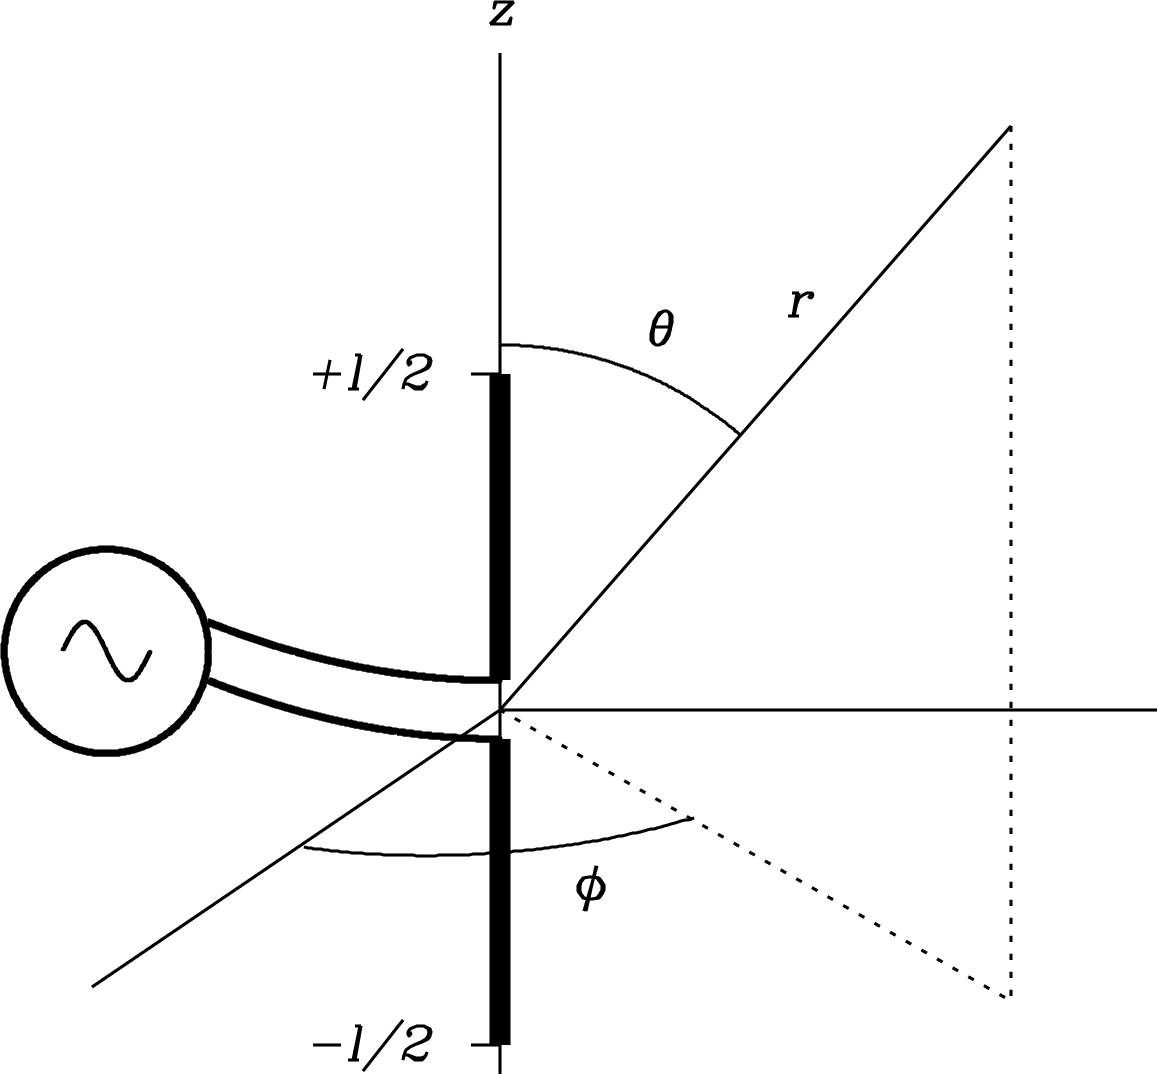
\includegraphics[width=0.5\textwidth]{short-dipole}
  \bicaption[短偶极天线示意图]{%
    分析短偶极天线的辐射所采用的坐标系统.
  }{%
    The coordinate system used to describe the radiation from a
    short dipole.
    \\\textcopyright{}
    \citeay{condon2016}, \S\,3.1.1.
  }
  \label{fig:short-dipole}
\end{figure}

\begin{figure}[htp]
  \centering
  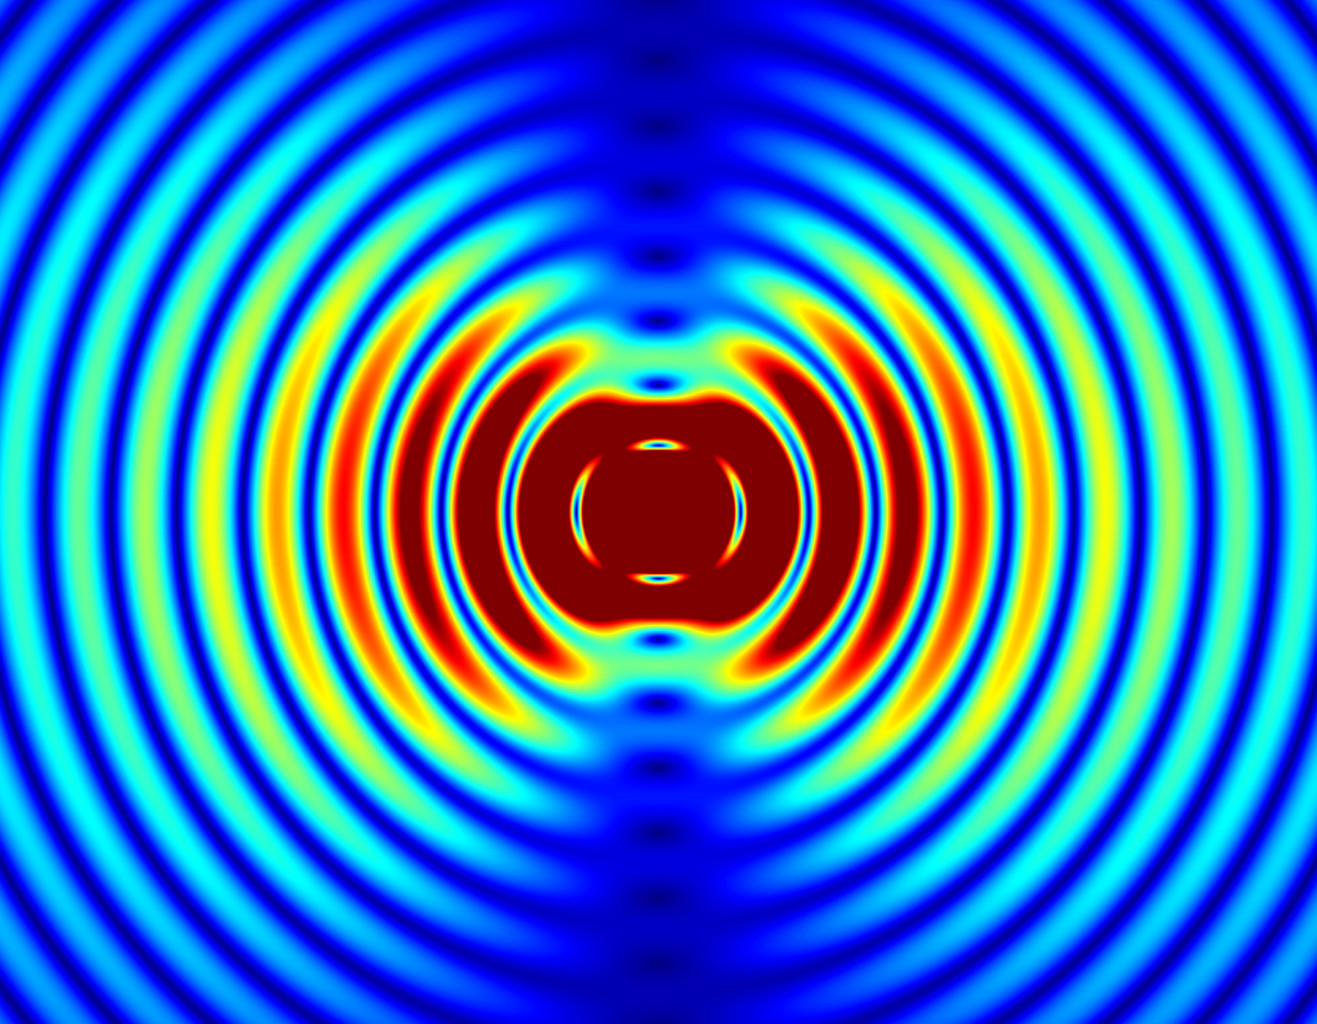
\includegraphics[width=0.6\textwidth]{hertzian-dipole-radiation}
  \bicaption[Hertz 偶极子的电场强度分布图]{%
    Hertz 偶极子的电场强度分布图.
  }{%
    The electric field intensity radiated from a Hertzian dipole.
    \\\textcopyright{}
    nageljr, \url{https://www.deviantart.com/nageljr/art/The-Hertzian-Dipole-Antenna-542377463}, (2019-03-18), \ac{cc} BY.
  }
  \label{fig:dipole-radiation}
\end{figure}

%---------------------------------------------------------------------
\subsection{功率方向图和增益}

\emph{\acf{pp}} $P(\theta,\phi)$ 是指一个天线的辐射功率的角向分布.
对于短偶极天线,由\autoref{eq:dipole-efield} 可得时间平均的
\emph{Poynting 流量}(即单位面积流过的功率)为:
\begin{equation}
  \label{eq:poynting-flux}
  \langle S \rangle
    = \frac{\acs{speed-light}}{4\Cpi} \langle E_{\bot}^2 \rangle
    = \frac{\Cpi}{8\,\acs{speed-light}}
      \left( \frac{I_0 l}{\lambda} \right)^2 \frac{\sin^2\theta}{r^2} .
\end{equation}
于是,归一化的\ac{pp}为:
\begin{equation}
  \label{eq:power-pattern}
  P(\theta,\phi) = \sin^2\theta .
\end{equation}
对于更普遍的情况,$P(\theta,\phi)$ 将与两个空间方位角 $(\theta, \phi)$
均相关.

\emph{\acf{gain}} $G(\theta,\phi)$ 定义为天线在方向 $(\theta, \phi)$
的辐射功率 $P(\theta,\phi)$ 与一个总辐射功率相等但各向辐射同性的天线的辐射功率
$\overline{P}$ 之比,即:
\begin{equation}
  \label{eq:gain}
  G(\theta,\phi) = \frac{P(\theta,\phi)}{\overline{P}}
    = \frac{4\Cpi P(\theta,\phi)}{\int P(\theta,\phi) \,\D{\Omega}} .
\end{equation}
可见,一个天线的\ac{gain}与其\ac{pp}只相差一个常数.

%---------------------------------------------------------------------
\subsection{主瓣}

天线的\ac{pp} $P(\theta,\phi)$ 通常会在一定方向范围明显大于在其他方向的值,
这个方向范围便称为天线的\emph{\acf{mainlobe}},
其余的称为\emph{\acf{sidelobe}},如\autoref{fig:lobes} 所示.
主瓣的立体角 $\Omega_{\R{MB}}$ 定义为:
\begin{equation}
  \label{eq:omega-mb}
  \Omega_{\R{MB}} = \int_{\R{MB}} P_n(\theta,\phi) \,\D{\Omega} ,
\end{equation}
其中 $P_n(\theta,\phi) \equiv P(\theta,\phi) / P_{\R{max}}$
为归一化的\ac{pp}.
主瓣的角度范围一般由\emph{\acf{hpbw}}描述,其定义为 $P(\theta,\phi)$
下降至最大值的一半时主瓣的两点之间的角距离,亦如\autoref{fig:lobes} 所示.

\begin{figure}[htp]
  \centering
  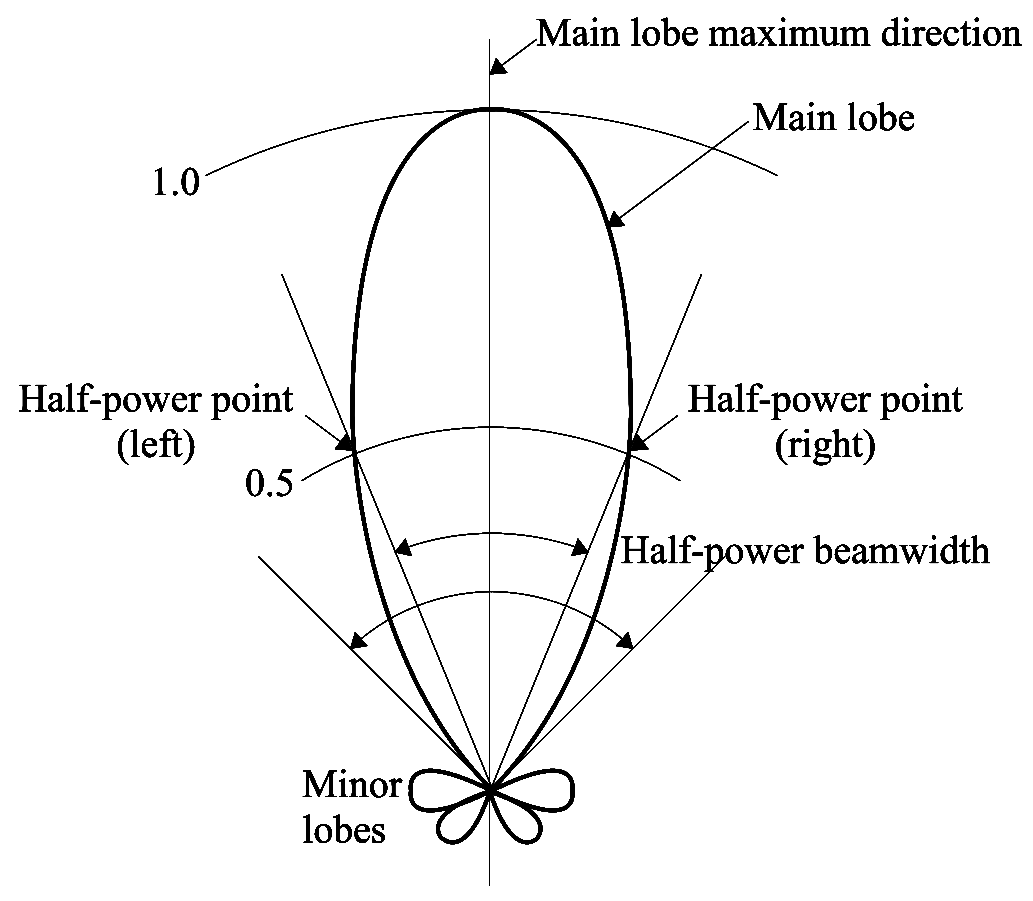
\includegraphics[width=0.6\textwidth]{antenna-lobes}
  \bicaption[天线的主瓣及其宽度示意图]{%
    天线的主瓣及其\acl*{hpbw}示意图.
  }{%
    Diagram of an antenna's main lobe and its HPBW.
    \\\textcopyright{}
    \citeay{zuniga2009}.
  }
  \label{fig:lobes}
\end{figure}

%---------------------------------------------------------------------
\subsection{有效接收面积}

若一个天线测量一个流量密度为 $S_{\nu}$ 的非偏振源输出的谱功率为 $P_{\nu}$,
则该天线的\emph{有效接收面积 (effective collecting area)} $A_e$ 定义为:
\begin{equation}
  \label{eq:area-eff}
  A_e \equiv \frac{2 P_{\nu}}{S_{\nu}} ,
\end{equation}
其中的因子 2 是因为单个天线只能响应一个偏振方向.

\begin{figure}[htp]
  \centering
  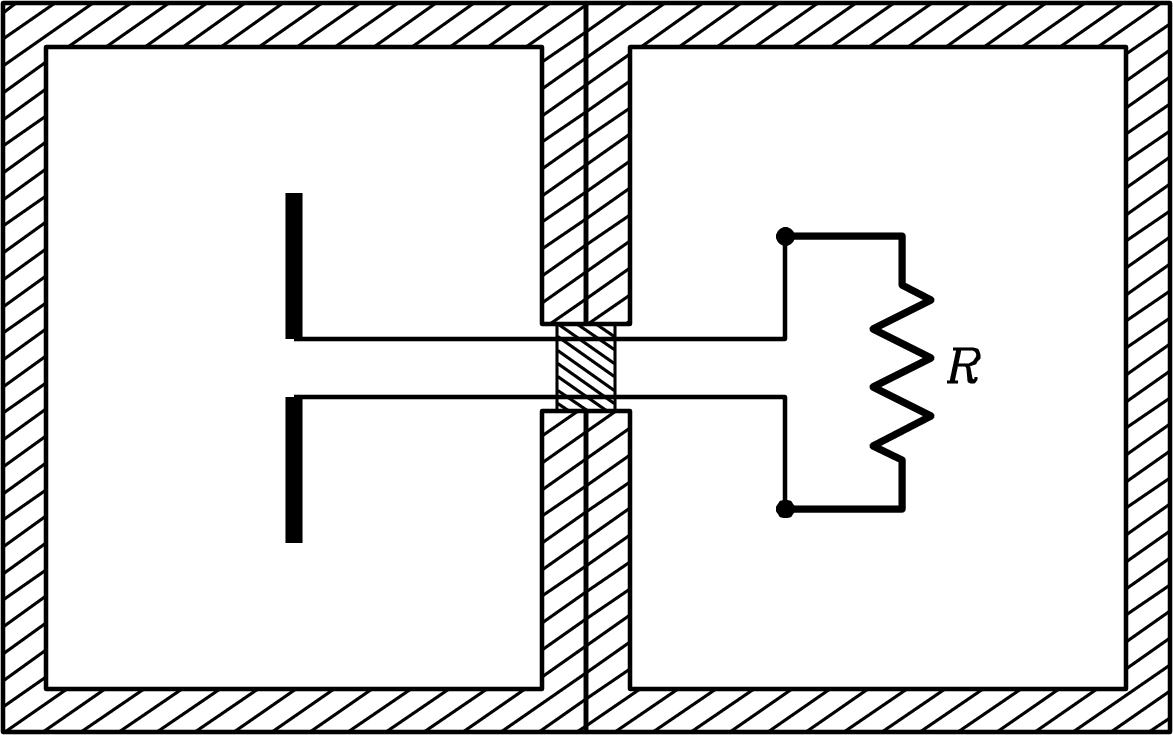
\includegraphics[width=0.5\textwidth]{average-area-thought-exp}
  \bicaption[计算天线平均接收面积的思想实验]{%
    计算天线平均接收面积 $\langle A_e \rangle$ 的思想实验.
  }{%
    A though experiment to calculate the average collection area
    $\langle A_e \rangle$.
    \\\textcopyright{}
    \citeay{condon2016}, \S\,3.1.4.
  }
  \label{fig:Aavg-thought-exp}
\end{figure}

一个天线的\emph{平均接收面积}为:
\begin{equation}
  \label{eq:area-avg1}
  \langle A_e \rangle
    \equiv \frac{1}{4\Cpi} \int A_e(\theta,\phi) \,\D{\Omega} .
\end{equation}
为计算该面积,可借助这样一个思想实验:
一个理想的无损天线和一个匹配的理想电阻,分别置于两个温度均为 $T$ 的空腔中而达到热平衡,
天线和电阻之间使用导线相连,两个空腔之间有一个特殊的阀门,能够阻挡电磁波,
但允许频率范围为 $[\nu, \,\nu+\D{\nu}]$ 的电流通过导线,
如\autoref{fig:Aavg-thought-exp} 所示.
因为整个系统处于热平衡状态,所以导线中没有\emph{净}能量流动,
否则其中一个空腔将升温、另一个则冷却,违背热力学第二定律.
因此,天线接收各方向的无偏振黑体辐射所产生的总谱功率为:
\begin{equation}
  P_{\nu,a} = \frac{1}{2} \int A_e(\theta,\phi) B_{\nu} \,\D{\Omega} ,
\end{equation}
该谱功率必须等于电阻产生的热噪声的谱功率 $P_{\nu,r}$.
代入\autoref{eq:nyquist} 和\autoref{eq:planck},可得
\begin{equation}
  \acs{kb}T = \frac{2\,\acs{kb}T}{2\lambda^2}
    \int A_e(\theta,\phi) \,\D{\Omega} .
\end{equation}
于是获得天线的平均接收面积 $\langle A_e \rangle$ 为:
\begin{equation}
  \label{eq:area-avg}
  \langle A_e \rangle = \frac{\lambda^2}{4\Cpi}.
\end{equation}

%---------------------------------------------------------------------
\subsection{天线温度}

一个被置于温度为 $T$ 的黑体辐射环境中的天线,
输出的噪声将与温度为 $T$ 的电阻所产生的热噪声 [\autoref{eq:nyquist-approx}]
是不可分辨的,该电阻被称为天线的\emph{匹配电阻}.
据此,可定义\emph{\ac{T-antenna}} 为其匹配电阻的温度,即
\begin{equation}
  \label{eq:t-ant}
  \acs{T-antenna} \equiv \frac{P_{\nu}}{\acs{kb}} .
\end{equation}
结合\autoref{eq:area-eff} 给出的有效接收面积,
一个流量密度为 $S_{\nu}$ 无偏振辐射源将使天线温度 \acs{T-antenna} 上升:
\begin{equation}
  \label{eq:dt-source}
  \Delta T = \frac{A_e S_{\nu}}{2\,\acs{kb}} .
\end{equation}


%=====================================================================
\section{干涉测量原理}
\label{sec:interferometry}

根据衍射原理,望远镜的角分辨率为 $\theta \sim \lambda / D$,
其中 $\lambda$ 为辐射信号的波长(对应于观测频率),$D$ 为望远镜的直径.
相比光学波段,射电信号的波长要长得多,为了实现足够好的角分辨率,
必须建造巨型的望远镜,如 \SI{100}{\meter} 口径的 \ac{gbt}、
\SI{305}{\meter} 口径的 Arecibo、
\SI{500}{\meter} 口径的 \ac{fast}.
然而,在数百 \si{\MHz} 的低频射电波段,望远镜的口径需达到惊人的 \SI{10}{\km}
才能在 \SI{100}{\MHz} 实现约 \SI{1}{\arcminute} 的角分辨率,
这对于单口径望远镜而言显然是不现实的.
因此,低频射电观测通常使用\emph{干涉测量}技术,通过联合一系列小望远镜开展相干测量并综合,
获得高分辨率图像.

%---------------------------------------------------------------------
\subsection{二元准单色干涉仪}

\begin{figure}[htp]
  \centering
  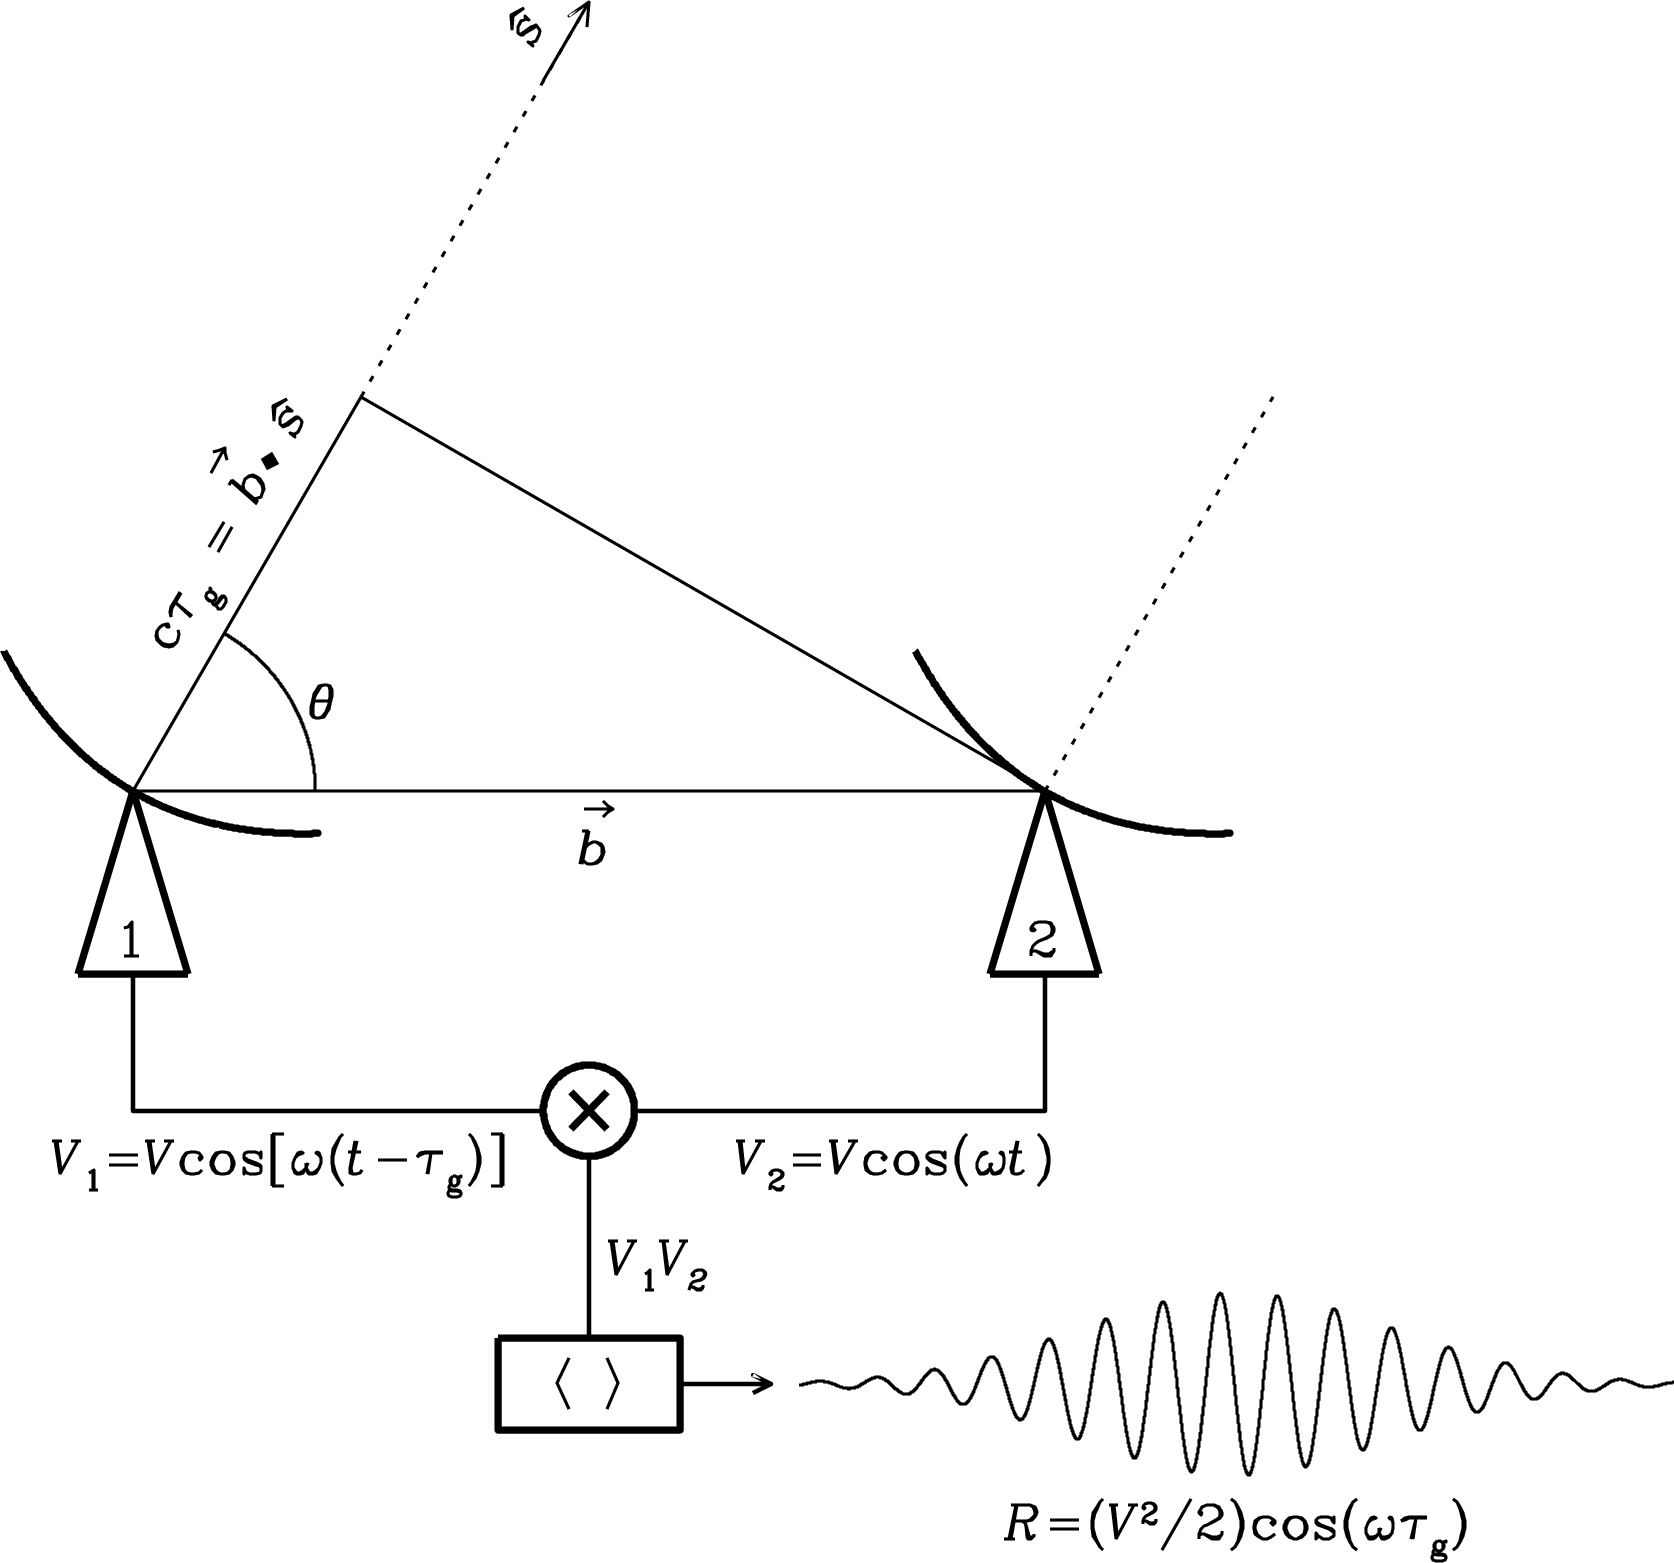
\includegraphics[width=0.7\textwidth]{interferometer}
  \bicaption[二元准单色干涉仪]{%
    二元准单色干涉仪的构成示意图.
    两个相同的天线相距 $\B{b}$ 放置并指向位于 $\hat{\B{s}}$ 方向的辐射源,
    接收的信号被放大后,再经过\acs*{ctor}的相乘($\times$)
    和时间平均($\langle\;\rangle$),得到输出响应 $R$.
  }{%
    The components of a two-element quasi-monochromatic interferometer
    observing in a very narrow radio frequency band centered at
    $\nu = \omega / (2\Cpi)$.
    The two identical antennas are separated by the baseline vector
    $\B{b}$ and point to the source in direction $\hat{\B{s}}$.
    The signals received by the antennas are amplified,
    multiplied ($\times$), and time averaged ($\langle\;\rangle$)
    by the correlator to yield the output response $R$.
    \\\textcopyright{}
    \citeay{condon2016}, \S\,3.7.1.
  }
  \label{fig:interferometer}
\end{figure}

考虑一个最简单的二元准单色干涉仪(如\autoref{fig:interferometer} 所示),
由两个相同的天线和相关器构成,只测量频率为 $\nu$ 的准单色信号.
由于辐射源非常遥远,其信号到达干涉仪时为平面波(忽略电离层扰动等影响).
同一个波面被两个天线接收之间存在一个时间差,即\emph{\acf{delay-geo}}:
\begin{equation}
  \acs{delay-geo} = \frac{\B{b} \cdot \hat{\B{s}}}{\acs{speed-light}},
\end{equation}
其中 \acs{speed-light} 是\acl{speed-light},
$\B{b}$ 为两天线之间的基线矢量(由天线 1 指向天线 2),
$\hat{\B{s}}$ 为指向辐射源的单位矢量.
两个天线接收信号后分别输出电压响应:
\begin{align}
  V_1(t) &= V \cos [\omega (t - \acs{delay-geo})], \\
  V_2(t) &= V \cos (\omega t),
\end{align}
其中 $\omega = 2\Cpi\nu$ 为角频率.
然后,\emph{\acf{ctor}}将两个天线的响应相乘:
\begin{align}
  V_1(t) V_2(t)
    &= V^2 \cos [\omega (t - \acs{delay-geo})] \cos (\omega t) \\
    &= \frac{1}{2} V^2 \left[ \cos (2\omega t - \omega \acs{delay-geo})
      + \cos (\omega \acs{delay-geo}) \right].
\end{align}
接着,\ac{ctor}再对相乘后的响应进行时间平均 [参见\autoref{eq:ctor-avgtime}]:
\begin{equation}
  \label{eq:resp-corr}
  R = \langle V_1(t) V_2(t) \rangle
    = \frac{1}{2} V^2 \cos (\omega \acs{delay-geo}).
\end{equation}
由于天线响应 $V_1$ 和 $V_2$ 正比于辐射源的电场强度以及天线的\ac{gain}
[参见\autoref{eq:gain}],
因此\ac{ctor}的响应 $R$ 正比于辐射源的流量密度 $S$
以及 $\sqrt{A_1 A_2}$,其中 $A_1$ 和 $A_2$ 为两个天线的有效接收面积
[参见\autoref{eq:area-avg}].

由于地球的自转,辐射源的方向 $\hat{\B{s}}$ 发生变化,
\acl{delay-geo} \acs{delay-geo} 也随之变化,
于是\ac{ctor}的输出 $R$ 出现正弦形式的振荡,即\emph{\acf{fringe}},
其相位为:
\begin{equation}
  \phi = \omega \acs{delay-geo}
    = 2\Cpi \left( \frac{b \cos\theta}{\lambda} \right),
\end{equation}
其中 $\theta$ 为方向 $\hat{\B{s}}$ 和基线矢量 $\B{b}$ 之间的夹角.
于是有
\begin{equation}
  \diff{\phi}{\theta} = 2\Cpi \left( \frac{b \sin\theta}{\lambda} \right),
\end{equation}
可得单个\ac{fringe}的宽度,即干涉仪的\emph{\acf{bw-synthesized}}:
\begin{equation}
  \label{eq:bw-synthesized}
  \acs{bw-synthesized} = \frac{\lambda}{b \sin\theta},
\end{equation}
此参数描述了干涉仪的角分辨能力.

天线的\ac{pp}描述了其响应随方向的变化情况,也被称为干涉仪的\emph{\acf{pb}},
将对输出 $R$ 产生调制,如\autoref{fig:interferometer} 所示,
其中\ac{ctor}的输出\ac{fringe}的包络示意了\ac{pb}的衰减情况.

对于一个表面亮度分布为 $\acs{I-nu}(\hat{\B{s}})$ 的\ac{src-extended},
由于不同位置产生的辐射互不相干,因此可以被当作一系列独立的点源处理,
于是上述二元准单色干涉仪的输出响应为:
\begin{align}
  \label{eq:resp-cos}
  R_c & = \int \acs{I-nu}(\hat{\B{s}})
      \cos \left( \omega \B{b}\cdot\hat{\B{s}} / \acs{speed-light} \right)
      \,\D{\Omega}  \\
    & = \int \acs{I-nu}(\hat{\B{s}}) \cos \left(
      2\Cpi\, \B{b}\cdot\hat{\B{s}} / \lambda \right) \,\D{\Omega},
\end{align}
其中下标 \enquote{$c$} 表示 \enquote{cosine} \ac{ctor}的输出,
以区分下文将要介绍的 \enquote{sine} \ac{ctor}.

一个任意的亮度分布 $I$ 可分解为奇对称成分 $I_O$ 与偶对称成分 $I_E$ 之和,
然而\autoref{eq:resp-cos} 描述的 cosine \ac{ctor}只能测量其中的
偶对称成分 $I_E$,即:
\begin{align}
  R_c & = \int \left[ I_O(\hat{\B{s}}) + I_E(\hat{\B{s}}) \right]
      \cos \left( 2\Cpi\, \B{b}\cdot\hat{\B{s}} / \lambda \right)
      \,\D{\Omega}  \\
    & = \int I_E(\hat{\B{s}}) \cos \left(
      2\Cpi\, \B{b}\cdot\hat{\B{s}} / \lambda \right) \,\D{\Omega}.
\end{align}
为了能够测量另一个奇对称成分 $I_O$,则需要一个 \enquote{sine} \ac{ctor},
可通过对其中一个天线的输出增加 $\Cpi/2$ 的相位延迟来实现,于是有:
\begin{align}
  R_s & = \int \left[ I_O(\hat{\B{s}}) + I_E(\hat{\B{s}}) \right]
      \sin \left( 2\Cpi\, \B{b}\cdot\hat{\B{s}} / \lambda \right)
      \,\D{\Omega}  \\
    & = \int I_O(\hat{\B{s}}) \sin \left(
      2\Cpi\, \B{b}\cdot\hat{\B{s}} / \lambda \right) \,\D{\Omega}.
\end{align}
\ac{cctor} 即为一对 cosine 和 sine \ac{ctor}的组合.
相应地,\emph{\acf{Vis}},简称\emph{\ac{vis}},可定义为:
\begin{align}
  \label{eq:vis}
  \acs{Vis}
    & \equiv R_c - \Ci\, R_s  \\
    & = \int I_{\nu}(\hat{\B{s}}) \exp
      (-2\Cpi\Ci\, \B{b}\cdot\hat{\B{s}} / \lambda) \,\D{\Omega}.
\end{align}

%---------------------------------------------------------------------
\subsection{有限带宽}

现在,将上述二元干涉仪推广至测量有限带宽的信号.
考虑一段中心频率为 $\nu_c$ 且宽度为 $\Delta\nu$ 的窄频带,
若辐射源的亮度以及天线的响应在此频带内基本不变,
则可知测量的\ac{vis} [\autoref{eq:vis}] 为:
\begin{align}
  \acs{Vis} &= \int \left[ \frac{1}{\Delta\nu}
        \int_{\nu_c-\Delta\nu/2}^{\nu_c+\Delta\nu/2}
        I(\hat{\B{s}}, \nu) \exp (-2\Cpi\Ci\, \nu\acs{delay-geo})
      \right] \,\D{\Omega} \\
    &\approx \int I_{\nu}(\hat{\B{s}}) \sinc (\Delta\nu\,\acs{delay-geo})
      \exp (-2\Cpi\Ci\, \nu_c\acs{delay-geo}) \,\D{\Omega},
  \label{eq:vis-bw}
\end{align}
其中 $\sinc(\cdot)$ 为归一化 sinc 函数,定义如下:
\begin{equation}
  \label{eq:sinc}
  \sinc(x) =
    \begin{cases}
      \sin(\Cpi x) / (\Cpi x), & \quad \text{if } x \neq 0, \\
      1, & \quad \text{if } x = 0.
    \end{cases}
\end{equation}
因此,干涉仪测得的\ac{fringe}幅度减弱至原来的
$\sinc(\Delta\nu\,\acs{delay-geo})$ 倍.
为了最小化该损失,可以给前导天线的输出信号增加\emph{\acf{delay-comp}},
如\autoref{fig:interferometer-tau0} 所示,并随地球自转而调节 \acs{delay-comp}
使其满足 $|\acs{delay-comp} - \acs{delay-geo}| \ll (\Delta\nu)^{-1}$.
在此情况下,到达\ac{ctor}时两个天线的信号的相位是同步的.
同时,满足 $\acs{delay-comp} = \acs{delay-geo}$ 的方向 $\hat{\B{s}}_0$
称为\emph{\acf{delay-center}}或\emph{\acf{phase-refpos}}.

\begin{figure}[htp]
  \centering
  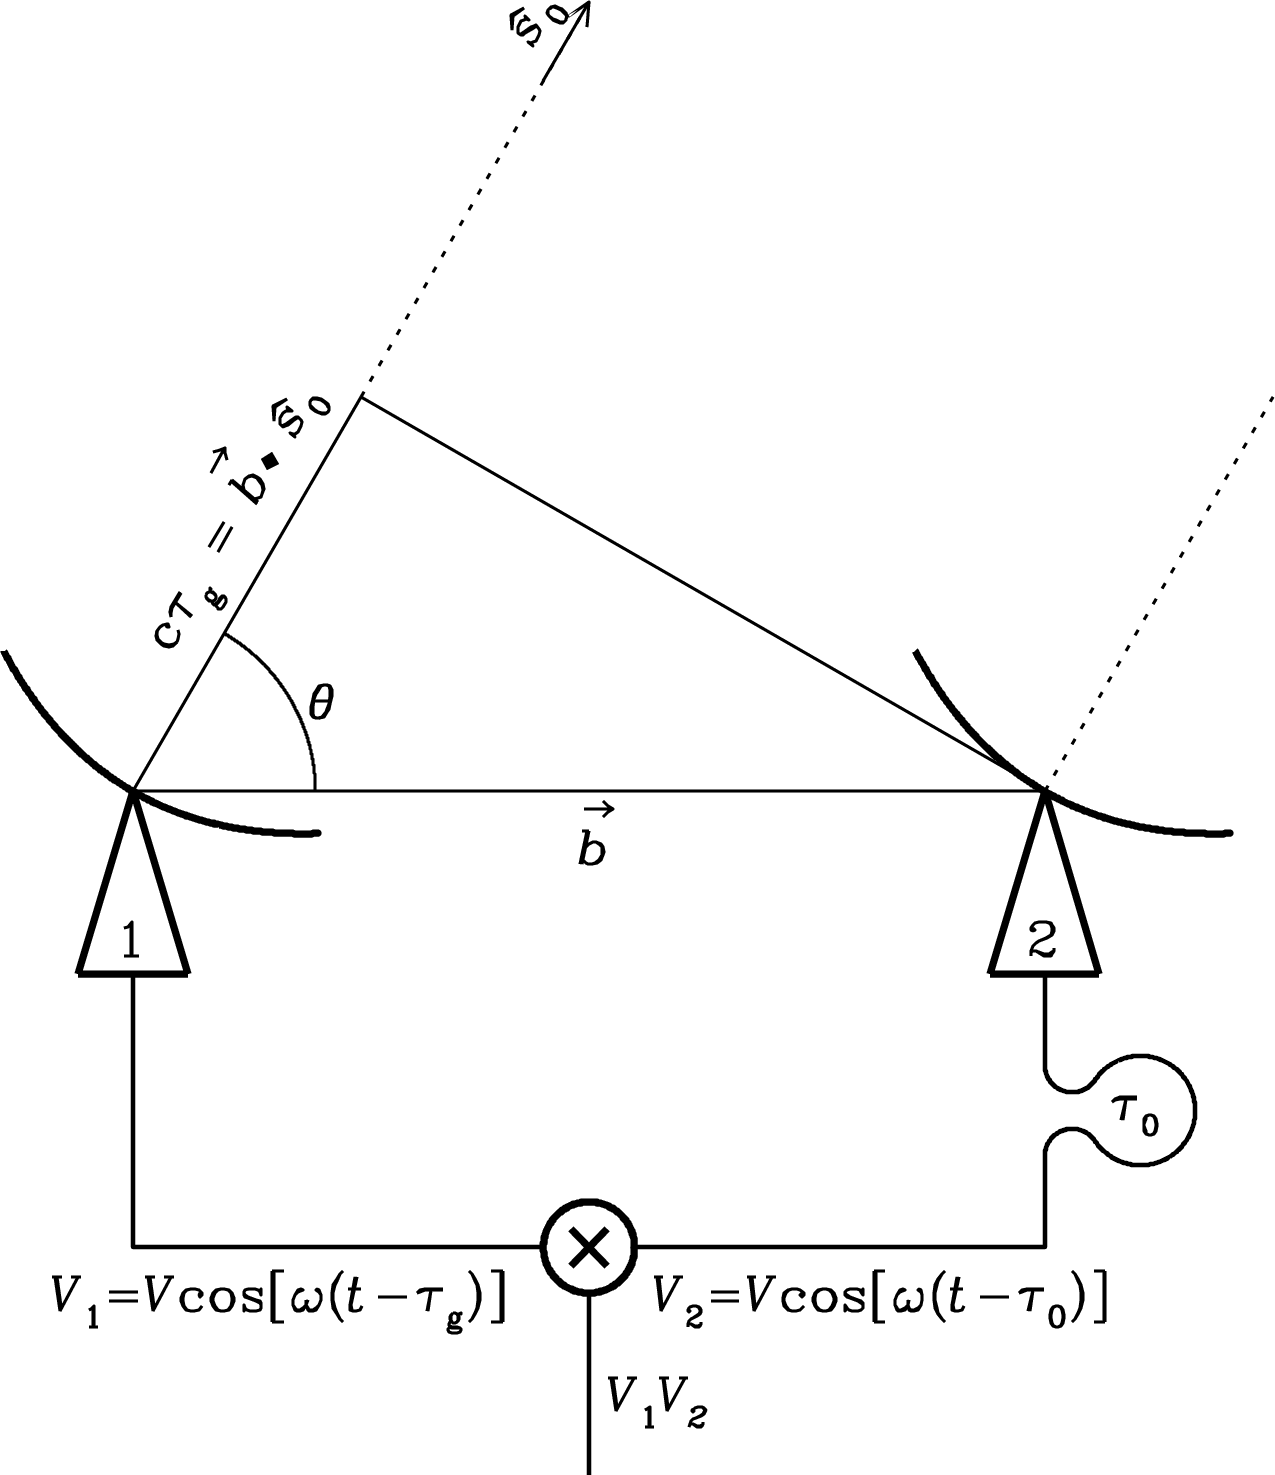
\includegraphics[width=0.6\textwidth]{interferometer-tau0}
  \bicaption[\acl*{delay-comp} \acs*{delay-comp}]{%
    通过给前导天线(即天线 2)增加\acl*{delay-comp}
    $\acs*{delay-comp} \approx \acs*{delay-geo}$,
    使得两天线的信号在相关运算时相位尽量同步,从而最小化带宽效应对测量条纹的衰减影响.
  }{%
    By introducing the compensating delay
    $\acs*{delay-comp} \approx \acs*{delay-geo}$ in the signal path of the
    leading antenna (i.e., antenna 2), the phases of the two signals are
    almost in sync when they reach the correlator, hence minimizing the
    attenuation to the measured fringes caused by the finite bandwidth
    effect.
    \\\textcopyright{}
    \citeay{condon2016}, \S\,3.7.3.
  }
  \label{fig:interferometer-tau0}
\end{figure}

\acl{delay-geo} \acs{delay-geo} 会随方向而变化,
因此\acl{delay-comp} \acs{delay-comp} 只对特定方向 $\hat{\B{s}}_0$
(即\ac{delay-center})是正好准确的.
偏离\ac{delay-center}的角度 $\Delta\theta$ 越大,
\acl{delay-comp} \acs{delay-comp} 的修正效果越差,
带宽带来的损失越大,即\emph{\acf{bw-smear}}.
该涂污效应限制了有效的视场大小,为满足:
\begin{equation}
  \Delta\nu \Delta\acs{delay-geo}
    \approx \Delta\nu \diff{\acs{delay-geo}}{\theta} \Delta\theta
    = \frac{b \sin\theta}{\acs{speed-light}} \Delta\nu \Delta\theta
    \ll 1,
\end{equation}
则要求:
\begin{equation}
  \Delta\theta \ll \frac{\nu \acs{bw-synthesized}}{\Delta\nu}.
\end{equation}
另一个解决\ac{bw-smear}的方法是将宽频带划分为一系列足够窄的频率通道
(如每个通道仅宽几十 \si{\kHz}),每个通道的信号都被独立地相关运算得到\ac{vis}.

类似地,如果\ac{ctor}的积分时间 $\Delta t$ 过长,则辐射源的位置 $\hat{\B{s}}$
会因地球自转而发生显著改变(可与 \acs{bw-synthesized} 相比拟),
导致\acl{delay-comp} \acs{delay-comp} 的修正效果变差,即\emph{\acf{t-smear}}.
一个距离\acl{delay-center} $\Delta\theta$ 的目标的移动速度为
$v = \omega_e \Delta\theta$,其中 $\omega_e$ 为地球自转的角速度.
为了最小化\ac{t-smear}的影响,\ac{ctor}的积分时间 $\Delta t$ 需满足:
\begin{equation}
  v \Delta t = \omega_e \Delta\theta \Delta t \ll \theta_s,
\end{equation}
即:
\begin{equation}
  \label{eq:ctor-avgtime}
  \Delta t \ll \frac{\theta_s}{\omega_e \Delta\theta}.
\end{equation}

%---------------------------------------------------------------------
\subsection{成像原理}

\begin{figure}[htp]
  \centering
  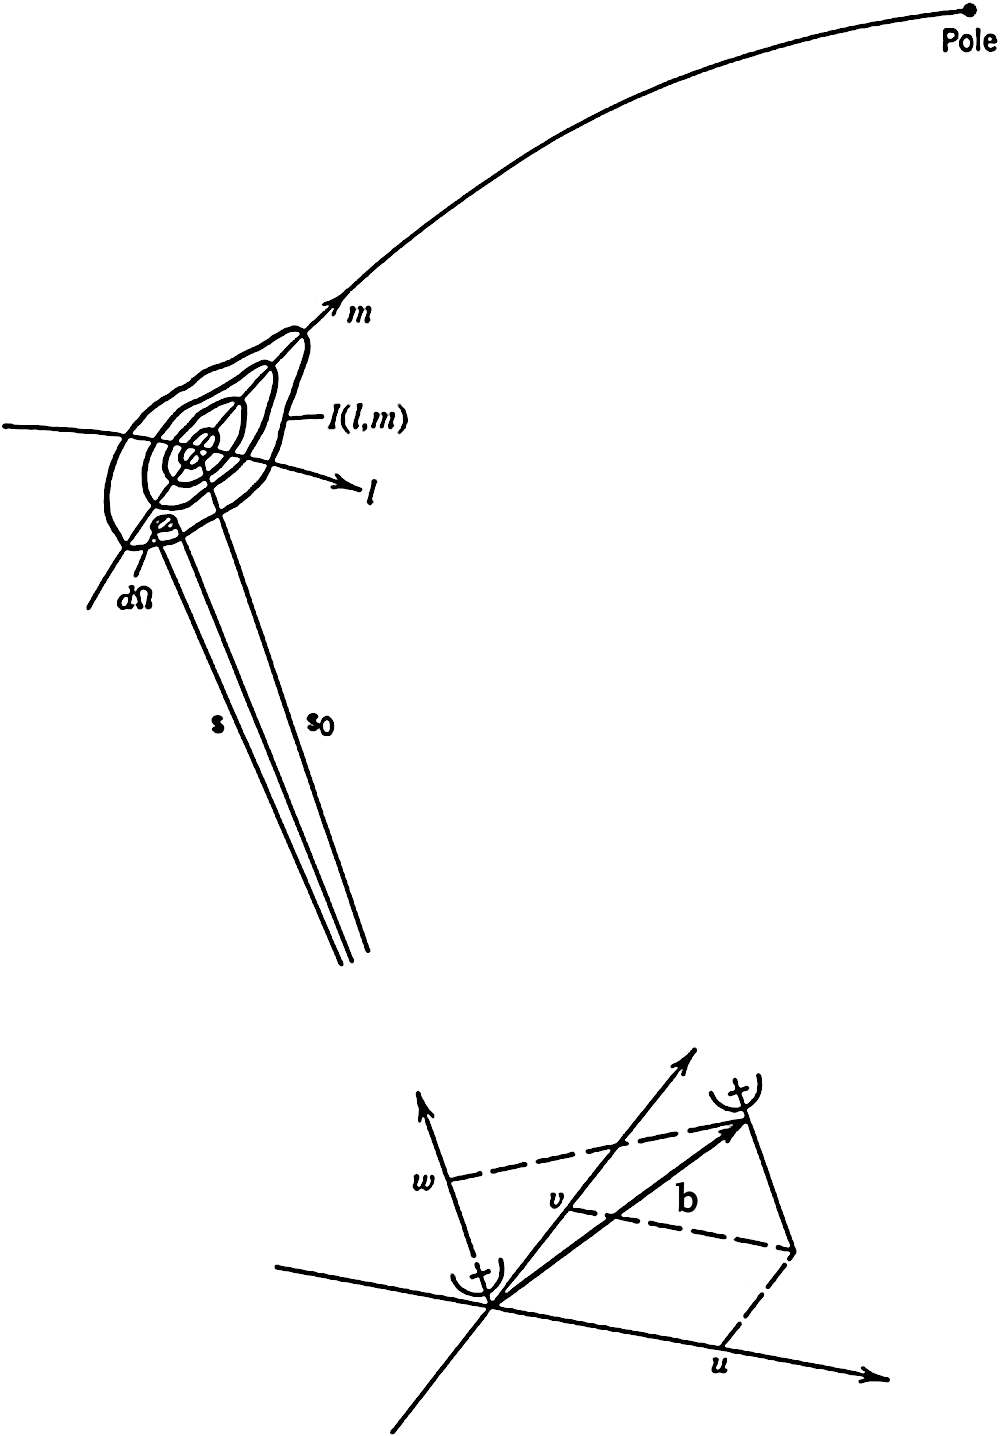
\includegraphics[width=0.7\textwidth]{interferometer-coordsys}
  \bicaption[$(u,v,w)$ 坐标系]{%
    干涉仪的 $(u,v,w)$ 直角坐标系,其中 $w$ 轴指向参考方向 $\hat{\B{s}}_0$,
    通常为目标的中心,$u$ 轴向东,$v$ 轴向北.
    基线矢量可表示为 $\B{b} = (u,v,w) \lambda$,
    目标的亮度分布则用\acs*{dc}描述,即 $I(\hat{\B{s}}) = I(l,m)$,
    其中 $l, m$ 为方向矢量 $\hat{\B{s}}$ 分别对 $u, v$ 轴的投影长度.
  }{%
    The $(u,v,w)$ Cartesian coordinate system for interferometers,
    in which the $w$-axis points in the reference direction
    $\hat{\B{s}}_0$ (usually toward the source center), and
    the $u$- and $v$-axes point east and north, respectively.
    A baseline vector is represented as $\B{b} = (u,v,w) \lambda$,
    and the source brightness distribution is described as
    $I(\hat{\B{s}}) = I(l,m)$, where $l, m$ are direction cosines,
    i.e., the projected lengths of the direction vector $\hat{\B{s}}$
    against the $u$- and $v$-axes, respectively.
    \\\textcopyright{}
    \citeay{thompson2017}, \S\,3.1.
  }
  \label{fig:interferometer-coordsys}
\end{figure}

为了能够实际运用\autoref{eq:vis} 或\autoref{eq:vis-bw} 获得图像,
需要定义一个坐标系,如\autoref{fig:interferometer-coordsys}
所示的 $(u,v,w)$ 直角坐标系是最常用的,其中 $w$ 轴指向参考方向 $\hat{\B{s}}_0$,
通常为目标的中心,$u$ 轴向东,$v$ 轴向北.
于是,基线矢量 $\B{b} = (u,v,w) \lambda$,
方向矢量 $\hat{\B{s}} = \left( l, m, \sqrt{1-l^2-m^2} \right)$,
其中 $l, m$ 为 $\hat{\B{s}}$ 分别对 $u, v$ 轴的投影长度,即\ac{dc}.
再利用 $\D{\Omega} = \D{l}\,\D{m} \,\big/ \sqrt{1-l^2-m^2}$,
\autoref{eq:vis} 可表示为:
\begin{equation}
  \label{eq:vis-uvw}
  \acs{Vis}(u,v,w) = \iint \frac{I_{\nu}(l,m)}{\sqrt{1-l^2-m^2}}
    \exp \left[ -2\Cpi\Ci \left( ul+vm+w\sqrt{1-l^2-m^2} \right) \right]
    \,\D{l}\,\D{m}.
\end{equation}
需注意,这\emph{不是}二维 Fourier 变换.

然而,在下述两种常见的特殊情况下,上式可变成二维 Fourier 变换,
从而通过逆运算获得目标的亮度分布.
\begin{itemize}
\item
\emph{所有基线矢量共面:}
这可进一步分为两种情形:
(1) 干涉阵列的天线只沿东西方向分布,如 \ac{wsrt},尽管地球自转,
所有基线矢量均落在同一垂直于地球自转轴的平面内;
(2) 虽然干涉阵列的天线分布在一个二维平面,如 \autoref{ssec:miteor}
将介绍的 \ac*{miteor},但只考虑瞬时观测.
此时,可以选取合适的坐标系使得 $w = 0$,于是\autoref{eq:vis-uvw}
变成二维 Fourier 变换,利用其逆变换可得目标的亮度分布为:
\begin{equation}
  \label{eq:vis-inv1}
  \frac{I_{\nu}(l,m)}{\sqrt{1-l^2-m^2}} = \iint \acs{Vis}(u,v, w \equiv 0)
    \exp [2\Cpi\Ci\, (ul+vm)] \,\D{l}\,\D{m}.
\end{equation}

%.......................................
\item
\emph{小视场成像:}
对于任何干涉阵列,如果只考虑以参考方向 $\hat{\B{s}}_0$ 为中心的足够小的区域,
于是有:
\begin{equation}
  w\sqrt{1-l^2-m^2} \approx w \left[ 1 - \frac{1}{2} (l^2+m^2) \right].
\end{equation}
则\autoref{eq:vis-uvw} 成为:
\begin{equation}
  \acs{Vis}(u,v,w) \approx \exp (-2\Cpi\Ci\,w) \iint
    \frac{I_{\nu}(l,m)}{\sqrt{1-l^2-m^2}}
    \exp [-2\Cpi\Ci\, (ul+vm) -\Ci\Cpi w(l^2+m^2)] \,\D{l}\,\D{m}.
\end{equation}
如果 $\big| \Cpi w(l^2+m^2) \big| \ll 1$,
即 $\exp [-\Ci\Cpi w(l^2+m^2)] \sim 1$,
则上式成为二维 Fourier 变换,即:
\begin{align}
  \acs{Vis}(u,v)
    & \equiv \acs{Vis}(u,v,w) \exp (2\Cpi\Ci\,w)  \\
    & = \iint \frac{I_{\nu}(l,m)}{\sqrt{1-l^2-m^2}}
    \exp [-2\Cpi\Ci\, (ul+vm)] \,\D{l}\,\D{m},
\end{align}
对其进行逆变换即可得到目标的亮度分布 $I_{\nu}(l,m)$:
\begin{equation}
  \label{eq:vis-inv2}
  \frac{I_{\nu}(l,m)}{\sqrt{1-l^2-m^2}} = \iint \acs{Vis}(u,v)
    \exp [2\Cpi\Ci\, (ul+vm)] \,\D{l}\,\D{m}.
\end{equation}

\end{itemize}

根据\autoref{eq:vis} 中基线矢量 $\B{b}$ 和方向矢量 $\hat{\B{s}}$ 之间的对称性,
上述第一种情况要求 $\B{b}$ 全部在同一平面内,
第二种情况要求 $\hat{\B{s}}$ 在天球上的对应点全部在同一平面内,即视场足够小,
因此,这两种情况可理解为相同近似条件的不同表现形式 \cite{clark1999}.
如果无法满足以上两种情况,比如大视场成像,则需要采用专门的成像方法
\cite{cornwell1992,sault2007},
比如 \ac{w-proj}法 \cite{cornwell2008}、\ac{w-stack}法 \cite{humphreys2011}
(将在 \autoref{ssec:imaging} 使用的 \texttt{WSClean} 成像软件实现了该方法
\cite{offringa2014,offringa2017}).

%---------------------------------------------------------------------
\subsection{\texorpdfstring{$uv$}{uv} 覆盖}

由于天空的亮度分布 $I_{\nu}(l,m)$ 为实数,因此测量的\ac{vis}满足
$\acs{Vis}(-u,-v) = \acs{Vis}^*(u,v)$,
于是基线矢量为 $\B{b} = (u,v,w)\lambda$ 的二元干涉仪在每个时刻测量
$uv$ 平面上两个相互对称的点的\ac{vis}.
随着地球自转,$\B{b}$ 的各分量逐渐变化,经过 \SI{24}{\hour},
该基线所测量的\ac{vis}数据对应 $uv$ 平面上两个相互对称的椭圆.
一个干涉阵列通常由大量天线组成,因此 $N_A$ 个天线之间可形成 $N_A(N_A-1)/2$ 条基线,
每条基线都将测量 $uv$ 平面上相应位置的\ac{vis},
可以显著增加 $uv$ 覆盖度,即 $uv$ 平面上被测量的点.
\autoref{fig:uv-coverages} 展示了不同天线数目、不同观测时长的 $uv$ 覆盖样例.

\begin{figure}[htp]
  \centering
  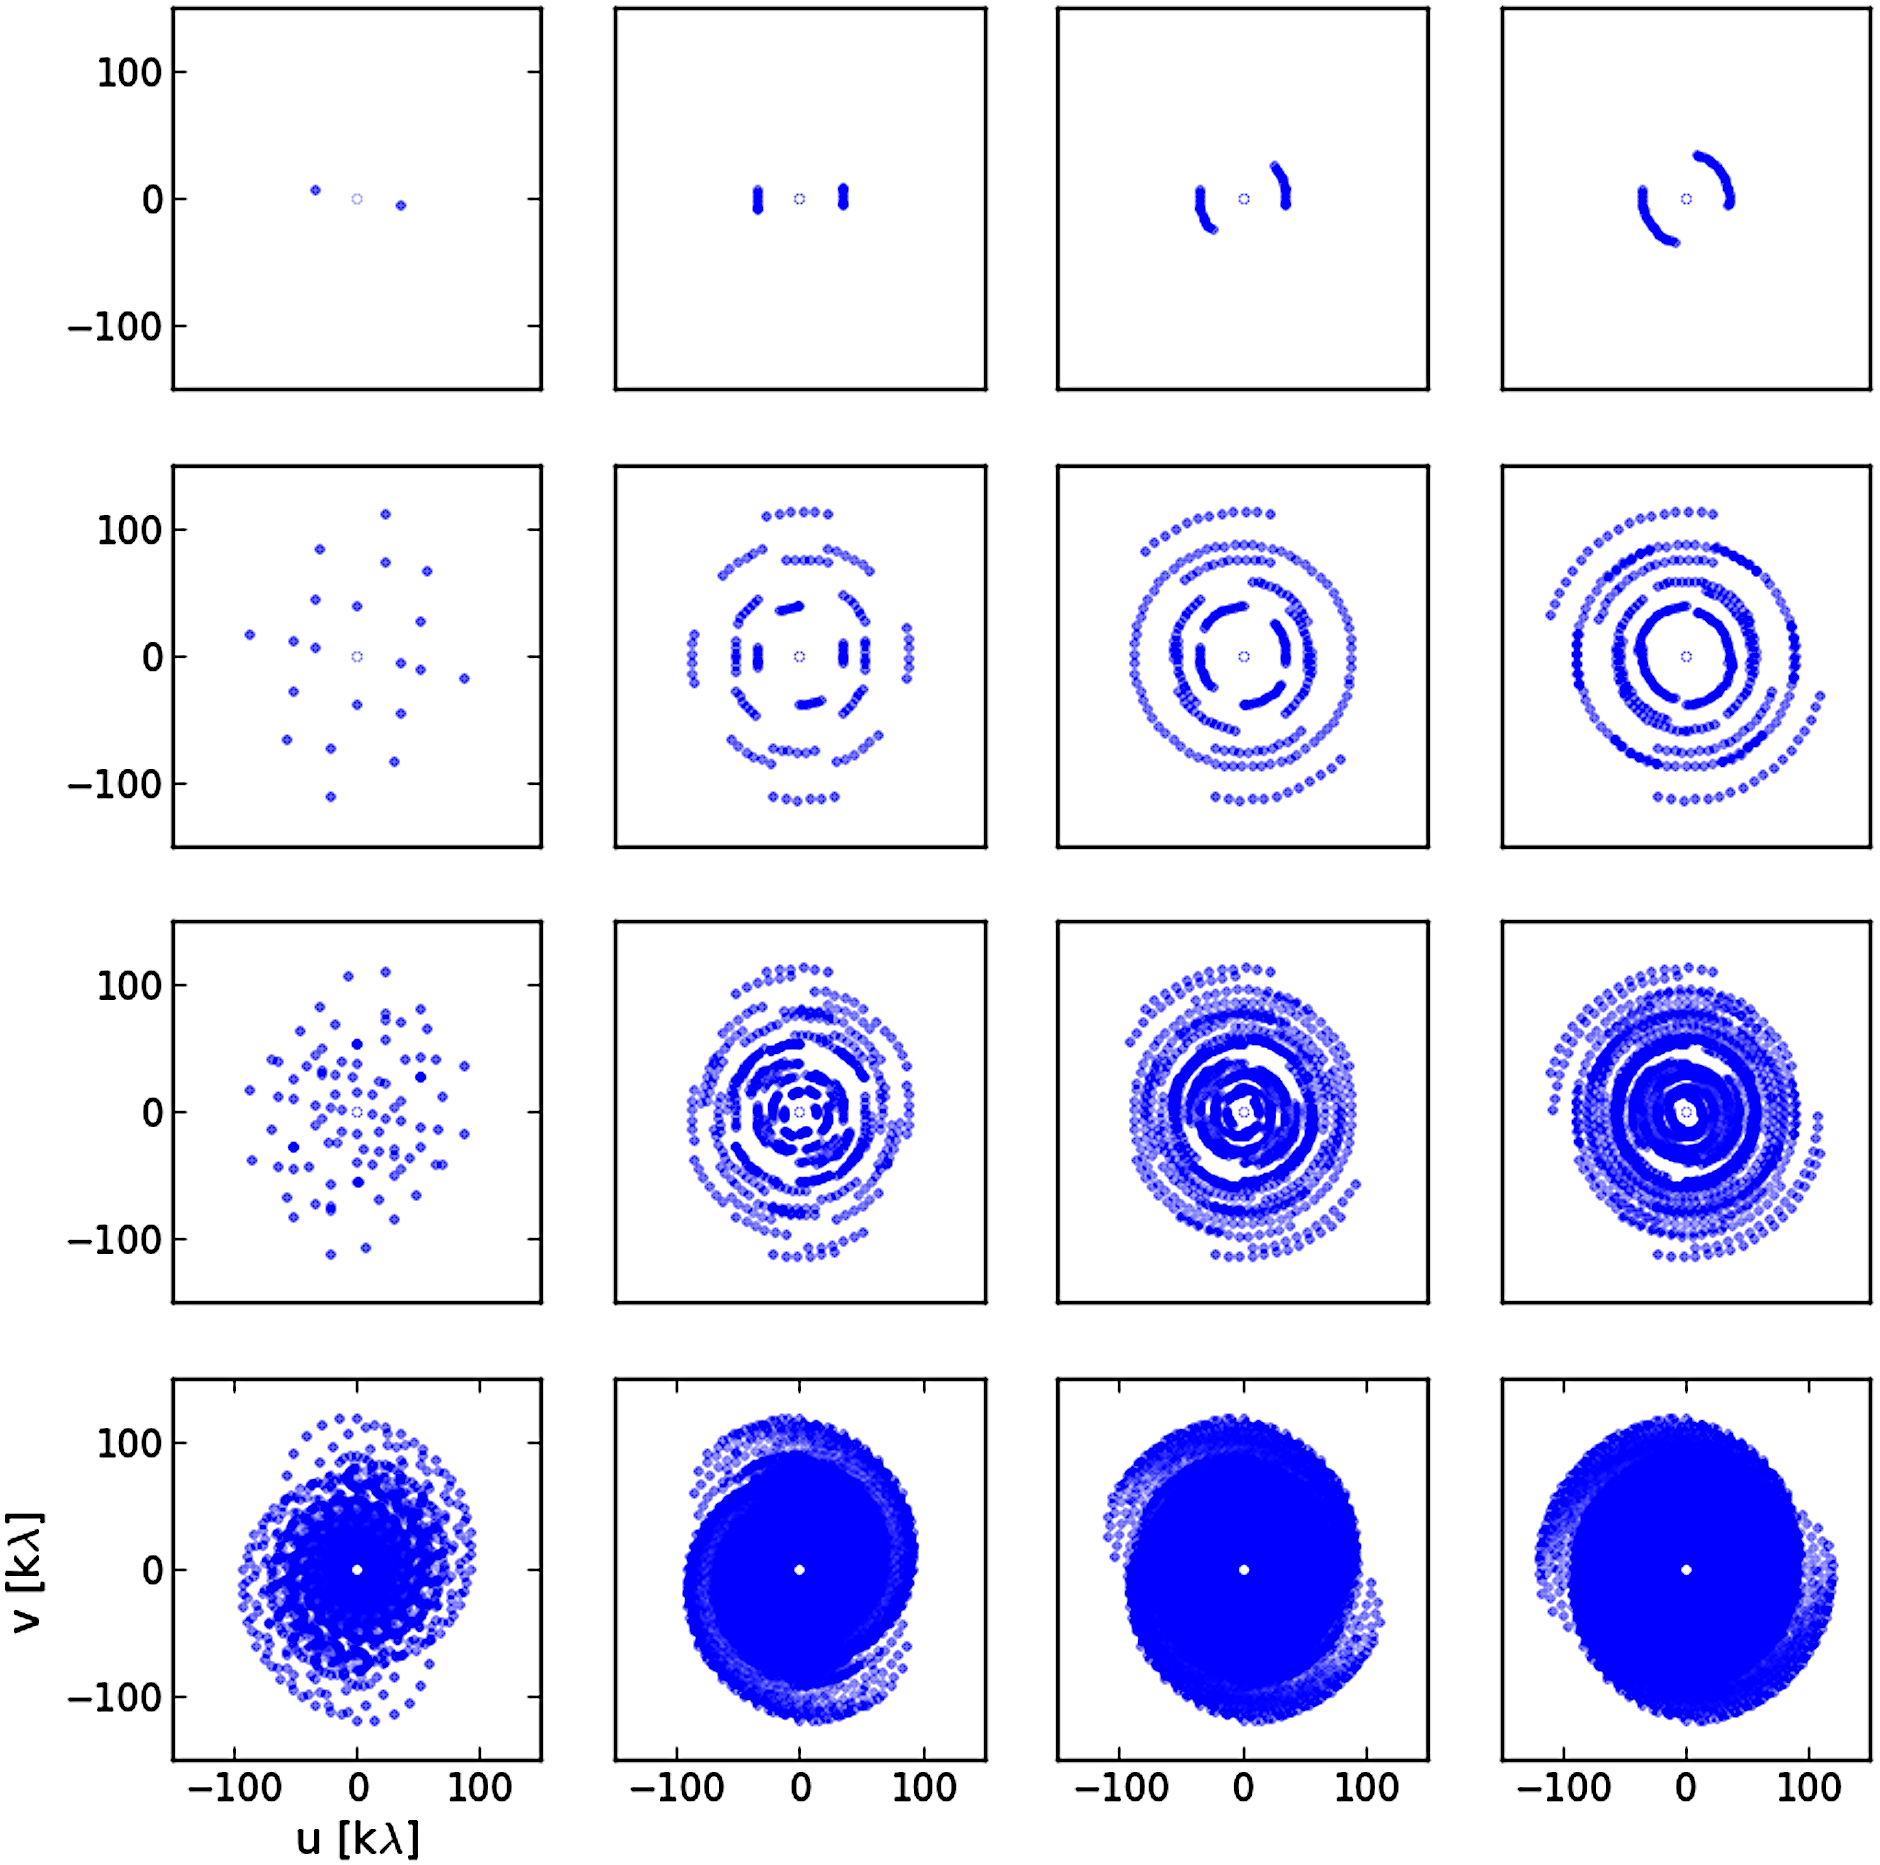
\includegraphics[width=\textwidth]{uv-coverages}
  \bicaption[$uv$ 覆盖样例]{%
    $uv$ 覆盖样例.
    \emph{从上往下:} 干涉阵列分别包括 2、5、10 和 50 个呈对数螺旋状分布的天线;
    \emph{从左到右:} 观测时间分别为 \SI{10}{\second}、\SI{2}{\hour}、
    \SI{4}{\hour} 和 \SI{6}{\hour}.
  }{%
    Examples of $uv$ coverages.
    \emph{Top to bottom:} the interferometer includes 2, 5, 10, and 50
    antennas in a logarithmic spiral pattern, respectively;
    \emph{Left to right:} the observing time is \SI{10}{\second},
    \SI{2}{\hour}, \SI{4}{\hour}, and \SI{6}{\hour}, respectively.
    \\\textcopyright{}
    \citeay{avison2013}.
  }
  \label{fig:uv-coverages}
\end{figure}

干涉阵列的天线数目总是有限的,在实际观测中 $uv$ 平面不可能被完全覆盖,
具体覆盖情况可由\emph{\acf{sf}}描述:
\begin{equation}
  \label{eq:sf}
  \acs{S-uv} = \sum_{k,t} \delta(u - u_{k,t}, v - v_{k,t}),
\end{equation}
其中 $u_{k,t}, v_{k,t}$ 为基线 $\B{b}_k$ 在 $t$ 时刻在 $uv$ 平面内的分量.
于是,干涉阵列实际测量的\ac{vis}数据为 $\acs{Vis}(u,v) \acs{S-uv}$,
由于无法获得目标亮度分布的全部信息,
根据\autoref{eq:vis-inv2} 对此进行逆 Fourier 变换
仅能得到目标的\emph{\acf{dirty-map}}:
\begin{equation}
  \label{eq:dirty-map}
  \frac{I_{\nu}^D(l,m)}{\sqrt{1-l^2-m^2}} = \iint
    \acs{Vis}(u,v) \acs{S-uv} \exp [2\Cpi\Ci\, (ul+vm)] \,\D{l}\,\D{m}.
\end{equation}
利用\ac{conv-theorem},上式可表示为:
\begin{equation}
  I_{\nu}^D(l,m) = I_{\nu}(l,m) * B(l,m),
\end{equation}
其中
\begin{equation}
  \label{eq:syn-beam}
  B(l,m) = \iint \acs{S-uv} \exp [2\Cpi\Ci\, (ul+vm)] \,\D{l}\,\D{m}
\end{equation}
是\ac{sf} \acs{S-uv} 的 Fourier 变换,
称为\emph{\acf{sb}}或\emph{\acf{psf}}.
\autoref{fig:imaging-relations} 展示了成像过程中各种变换关系.
为了从\ac{dirty-map} $I_{\nu}^D$ 尽可能地恢复目标的真实图像,
则需要使用复杂的非线性\ac{deconv}方法,
比如 CLEAN 算法 \cite{hogbom1974,cornwell1999}、
\ac{mem} \cite{narayan1986}.

\begin{figure}[htp]
  \centering
  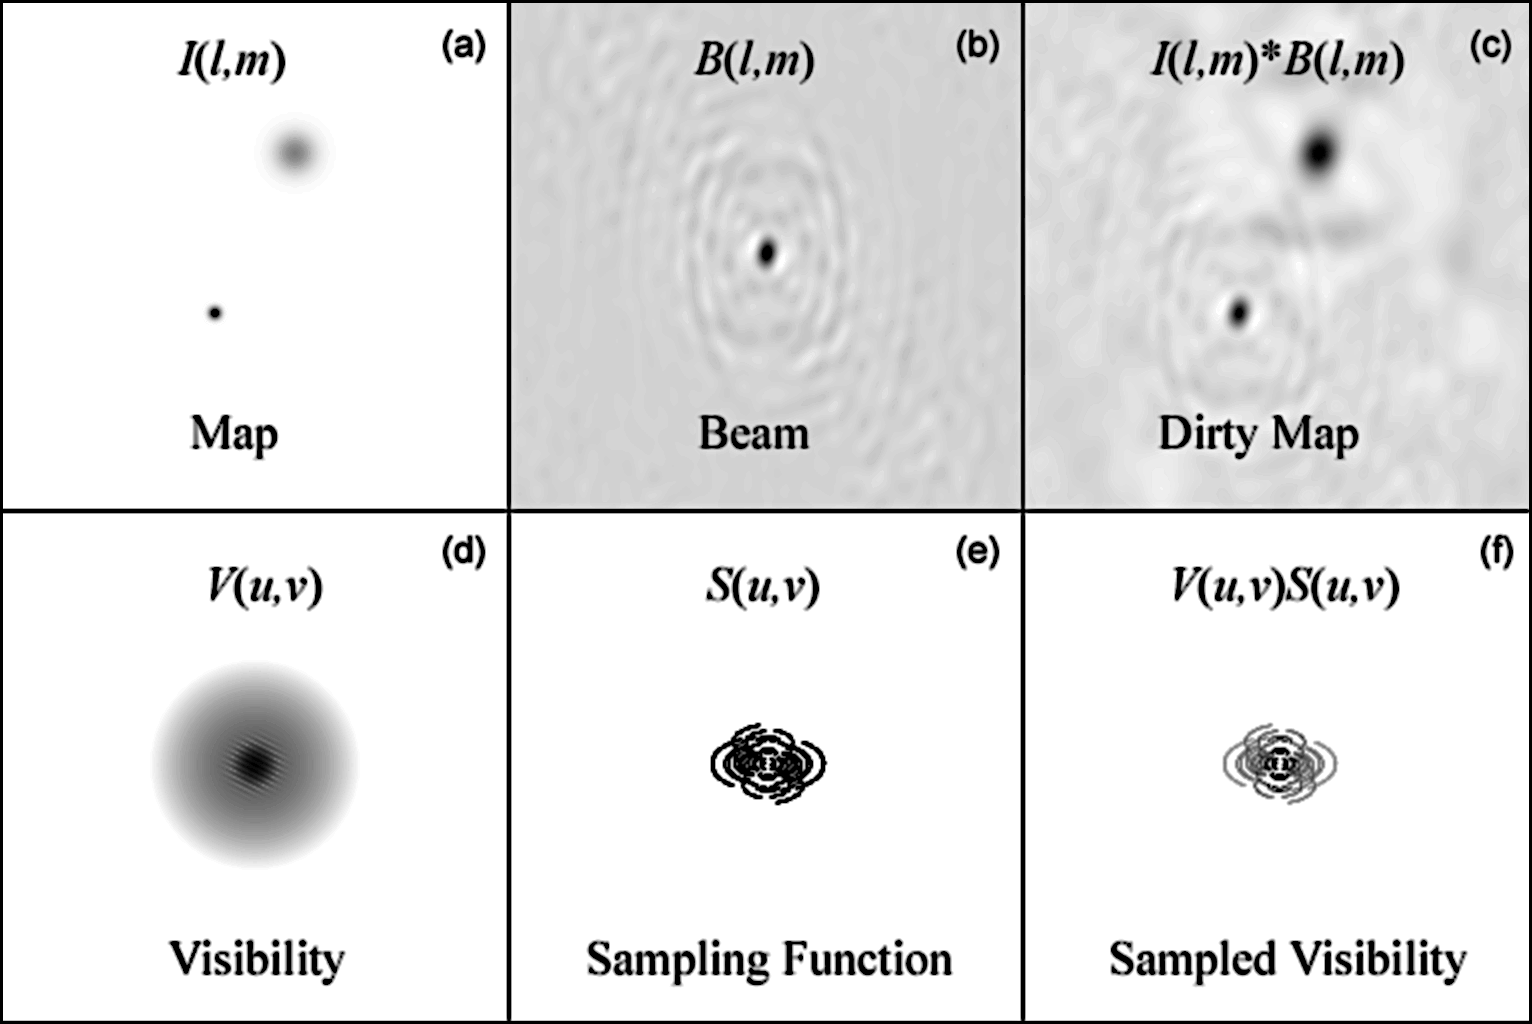
\includegraphics[width=\textwidth]{imaging-relations}
  \bicaption[成像过程中的变换关系]{%
    成像过程中的各种变换关系.
    \emph{(a)} 天空的真实图像;
    \emph{(b)} 干涉阵列的\acs*{sb},对应 (e) 的 Fourier 变换;
    \emph{(c)} 脏图,对应 (f) 的 Fourier 变换;
    \emph{(d)} \acs*{vis}的真实数据,对应 (a) 的 Fourier 变换;
    \emph{(e)} 干涉阵列的\acs*{sf};
    \emph{(f)} 实际测量到的\acs*{vis}数据,为 (d) 和 (e) 乘积.
  }{%
    The transform relations among the imaging process.
    \emph{(a)} The true sky map;
    \emph{(b)} The synthesized beam of the interferometer, which is the
    Fourier Transform of (e);
    \emph{(c)} The dirty map, which is the Fourier Transform of (f);
    \emph{(d)} The true visibility data, which are the Fourier Transform
    of (a);
    \emph{(e)} The sampling function of the interferometer;
    \emph{(f)} The actually measured visibility data, which are the
    product of (d) and (e).
    \\\textcopyright{}
    Dale E. Gary, Radio Astronomy, Lecture 6,
    \url{https://web.njit.edu/~gary/728/Lecture6.html}, (2018-11-21).
    [反转了颜色]
  }
  \label{fig:imaging-relations}
\end{figure}

%---------------------------------------------------------------------
\subsection{灵敏度}

考虑一个噪声功率的等效温度为 $T_s$ 的天线,其每个测量值的\ac{rms}误差为
$\sigma \approx \sqrt{2} T_s$
[详见 \citeay{condon2016}, 附录 B.6].
设信号的带宽为 $\Delta\nu$,根据\emph{采样定理 (sampling theorem)},
在时间 $\tau$ 内应采样 $N \gtrsim 2 \Delta\nu \,\tau$ 个数据点.
于是,对时间平均后的测量值的涨落为:
\begin{equation}
  \label{eq:radiometer}
  \sigma_T = \frac{\sqrt{2} T_s}{\sqrt{N}}
    \approx \frac{T_s}{\sqrt{\Delta\nu \,\tau}} ,
\end{equation}
其中 $\tau$ 为\ac{t-int}.
$\tau$ 越大,$\sigma_T$ 越小,则达到的灵敏度越高.
然而在实际情况中,多种系统误差会限制灵敏度的提高,
比如天线和接收机的\ac{gain}变化、大气层辐射的不规则涨落、
未分辨背景源产生的\ac{confusion}、等等。

若一个点源的辐射使天线的温度 $T_s$ 升高了 $\Delta T$,
则根据\autoref{eq:dt-source} 可测得该点源的流量密度为:
\begin{equation}
  S_{\nu} = \frac{2\,\acs{kb} \Delta T}{A_e} ,
\end{equation}
相应的测量误差为:
\begin{align}
  \sigma_S
    & = \frac{2\,\acs{kb}}{A_e} \sigma(T_s + \Delta T) \\
    & \approx \frac{2\,\acs{kb}}{A_e} \sigma(T_s) \\
    & = \frac{2\,\acs{kb} T_s}{A_e \sqrt{\Delta\nu \,\tau}} .
\end{align}
此即单天线的\emph{点源灵敏度}.

对于由两个相同天线构成的二元干涉仪,其点源灵敏度为:
\begin{equation}
  \label{eq:sigma-ps1}
  \sigma_S = \frac{\sqrt{2}\,\acs{kb} T_s}{A_e \sqrt{\Delta\nu \,\tau}} .
\end{equation}
由 \acs{N-ant} 个相同天线构成的干涉仪可形成 $\acs{N-ant}(\acs{N-ant}-1)$
个独立的二元干涉仪,因此其\emph{点源灵敏度}为:
\begin{equation}
  \label{eq:sigma-ps}
  \sigma_S = \frac{2\,\acs{kb} T_s}{
    A_e \sqrt{\acs{N-ant}(\acs{N-ant}-1) \Delta\nu \,\tau}} .
\end{equation}

如果观测一个\acf{src-extended},则需要考虑干涉仪的\emph{亮度灵敏度},
可利用 Rayleigh--Jeans 近似 [\autoref{eq:rj-approx}]
直接由 $\sigma_S$ 导出:
\begin{equation}
  \label{eq:sigma-tb}
  \sigma_b = \frac{\lambda^2}{2\,\acs{kb}} \frac{\sigma_S}{\Omega_A} ,
\end{equation}
其中 $\Omega_A$ 是波束的立体角.
相比单口径望远镜,干涉仪的基线长、角分辨率高,
因此\ac{sb}的立体角 $\Omega_A$ 非常小,
从而导致其亮度灵敏度 $\sigma_b$ 明显差于单口径望远镜.


%=====================================================================
\section{主要低频干涉阵列}
\label{sec:instruments}

大型低频干涉阵列是目前测量 EoR 信号的主要设备.
近十几年以来,国内外已建成一批各具特色的低频干涉阵列,
还有若干新型干涉阵列正在兴建或准备建设.
以下对其中主要的干涉阵列作简要介绍.

%---------------------------------------------------------------------
\subsection{21CMA}

\acf{21cma} 是我国开展“宇宙第一缕曙光”探测的低频射电干涉阵列,
位于中国西部天山深处的乌拉斯台,环绕在四周的高山能提供宁静的射电环境.
\acs{21cma} 的 81 个站点呈 T 形分布在东西约 \SI{6}{\km}、
南北约 \SI{4}{\km} 的两条直线上.
\autoref{fig:21cma} 展示了沿东西方向的部分站点.
每个站点包含 127 根对数周期天线,工作频率为 \SIrange{50}{200}{\MHz},
频率分辨率为 \SI{24.4}{\kHz},
角分辨率达 \SI{1}{\arcminute}(在 \SI{200}{\MHz} 处),
采用模拟波束合成固定观测以北天极为中心、半径约 \SI{5}{\degree} 的天区
\cite{wang2013,zheng2016}.
\acs{21cma} 已于 2006 年建设完成,并于 2009 年升级了新型低噪声放大器和
基于 \acs{gpu} 的数据采集系统,目前已积累多年的观测数据.
\acs{21cma} 作为中国主要的 \acs{ska} 探路者项目,
项目成员开发了完整的数据处理流程及软件、
提出了射频干涉探测及抑制新方法 \cite{huang2016}、
探测并编录了北天极视场内的 624 个射电源 \cite{zheng2016}.
目前,\acs{21cma} 正在改造升级数字多波束合成系统,
以实现多目标跟踪观测,掌握低频脉冲星的搜寻技术.

\begin{figure}[htp]
  \centering
  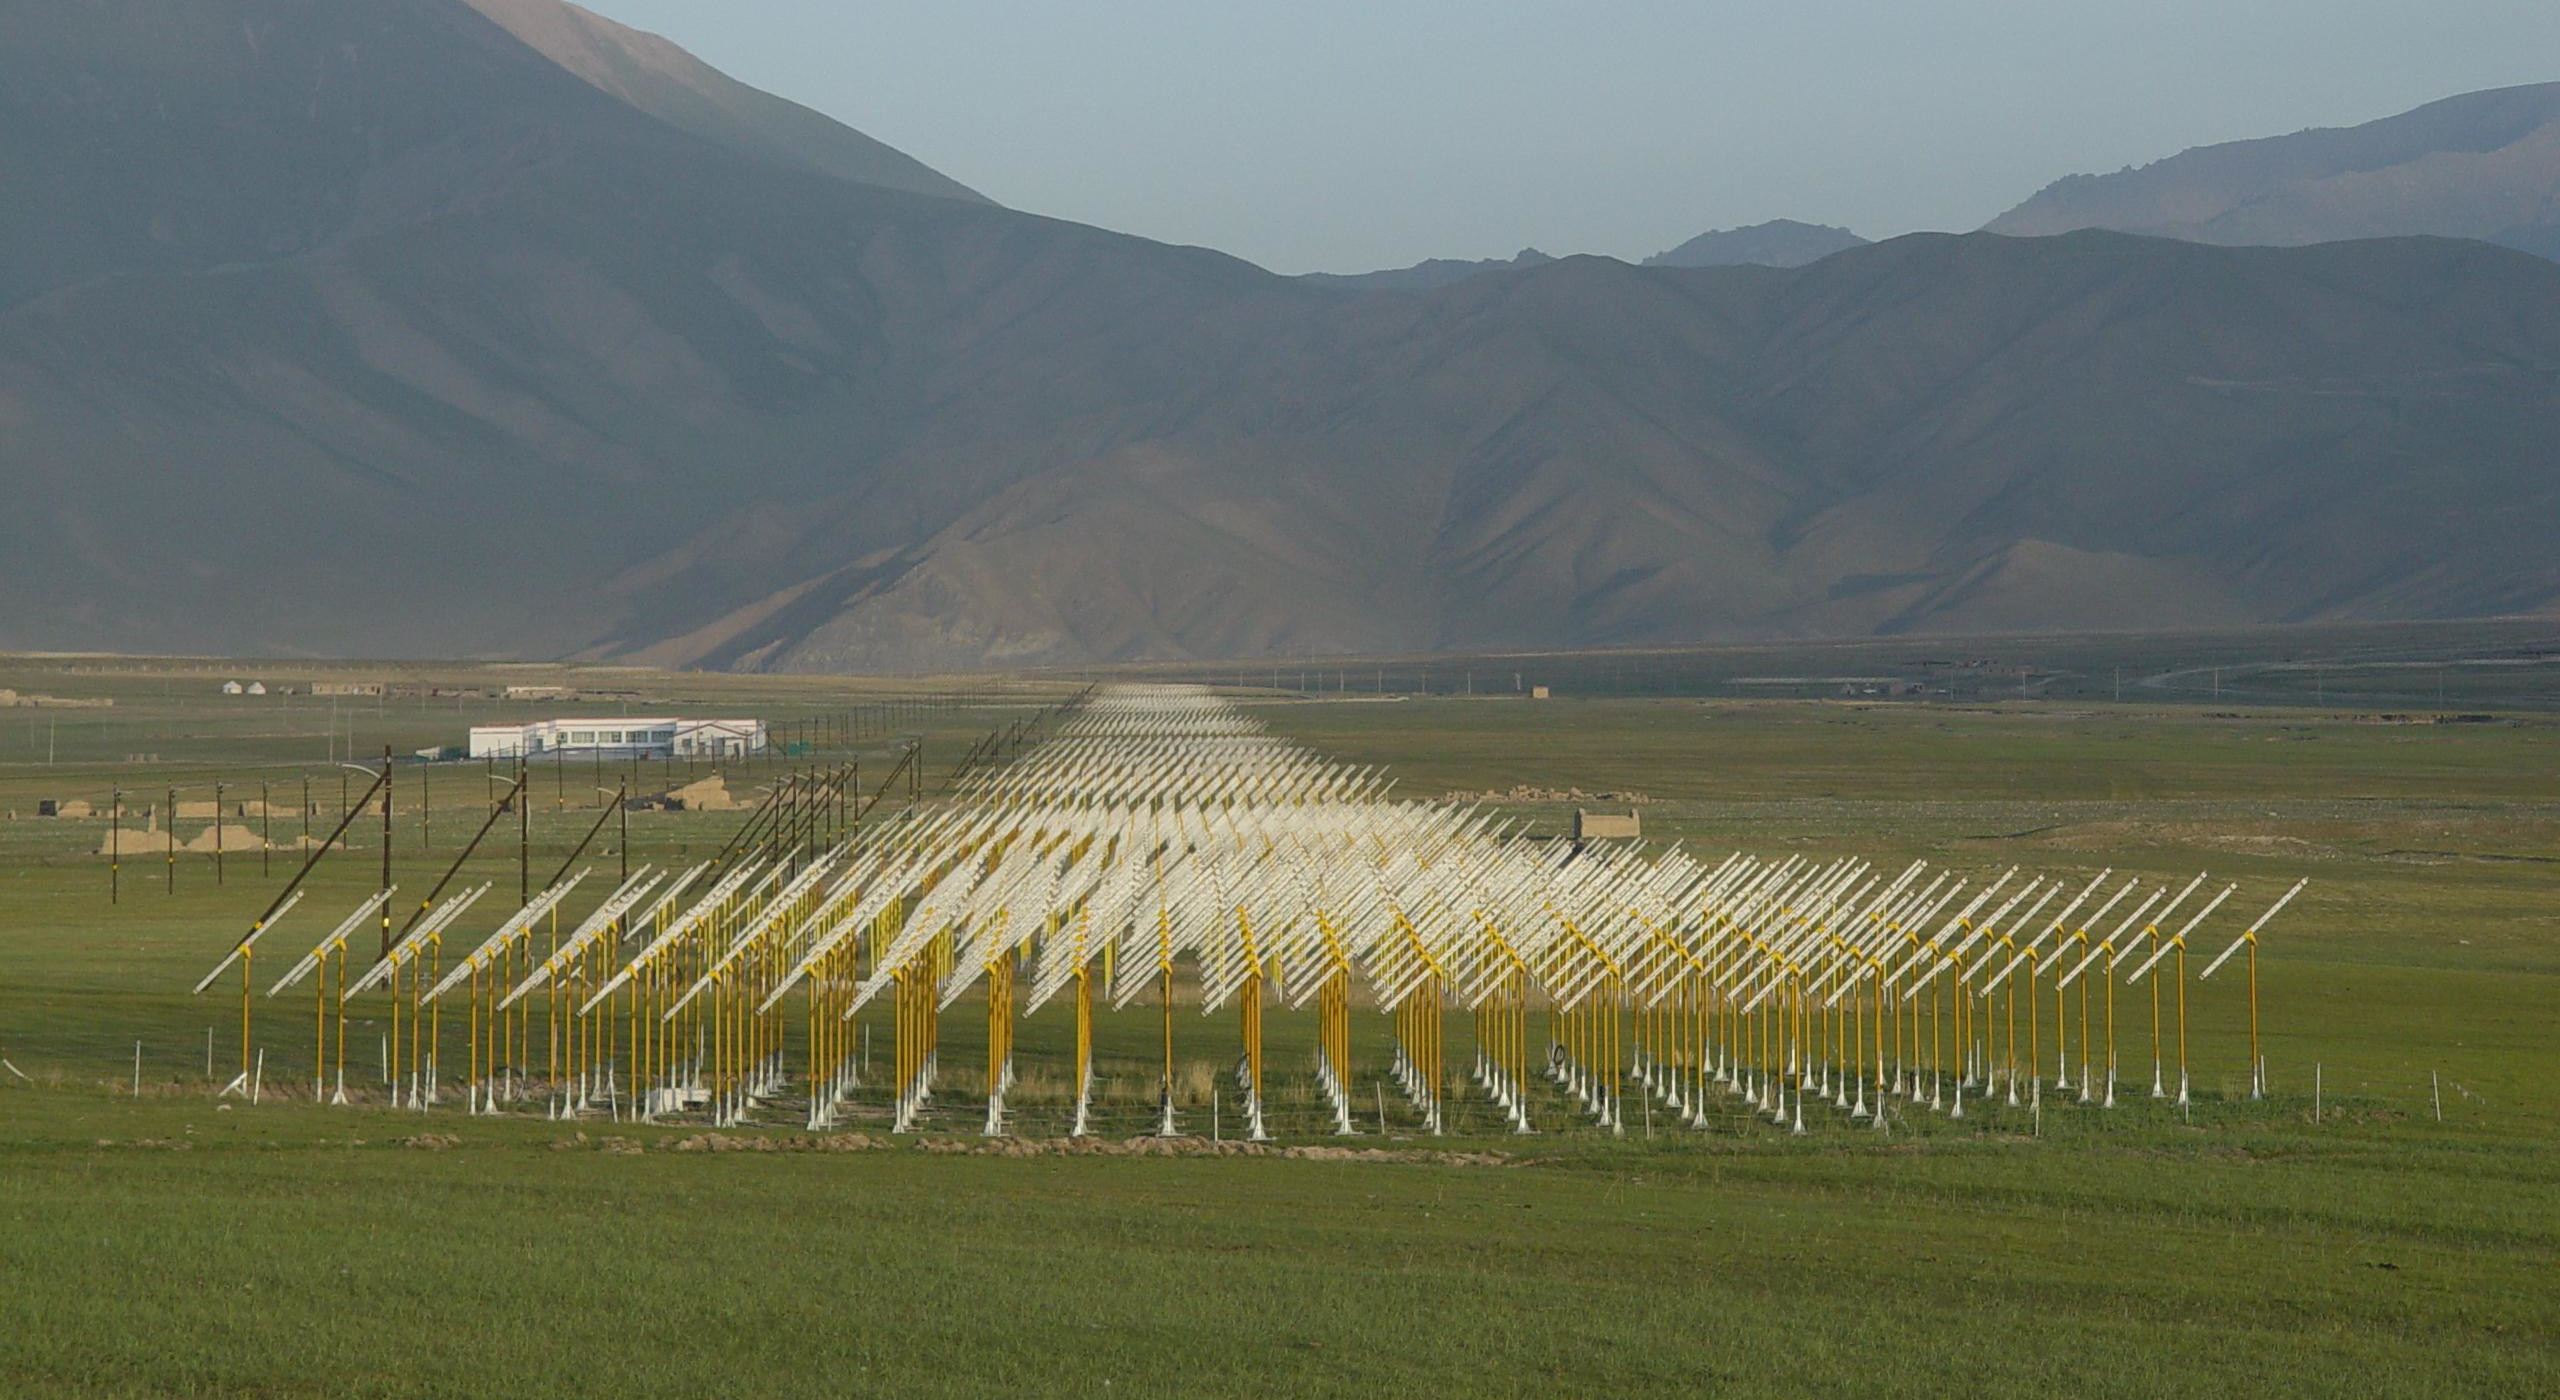
\includegraphics[width=0.8\textwidth]{21CMA}
  \bicaption[21CMA 东西方向的部分站点]{%
    21CMA 东西方向的部分站点,每个站点包含 127 根对数周期天线.
  }{%
    Part of the 21CMA stations along the east-west direction,
    with each station including 127 log-periodic antennas.
    \\\textcopyright{}
    21CMA, \acuse{nao}\acl{nao}.
  }
  \label{fig:21cma}
\end{figure}

%---------------------------------------------------------------------
\subsection{LOFAR}

\acf{lofar} 是由 \ac{astron} 建造的新型低频干涉阵列 \cite{vanHaarlem2013},
由工作在 \SIrange{10}{90}{\MHz} 波段的低频段天线(LBA)和
工作在 \SIrange{110}{250}{\MHz} 波段的高频段天线(HBA)两部分组成.
\acs{lofar} 共有 51 个站点,
其中 24 个站点分布在半径 \SI{2}{\km} 的核心区域
(\autoref{fig:lofar} 显示了最中心的部分),
14 个站点呈螺旋状分布在外围区域,
还有 13 个国际站点分布在德国、法国、瑞士、英国、波兰和爱尔兰,
基线长达 \SI{1500}{\km}.
荷兰境内的 38 个站点各包含 96 个 LBA 和 48 个 HBA,
13 个国际站点每个包含 96 个 LBA 和 96 个 HBA.
\acs{lofar} 采用了数字多波束合成技术,能实现多目标跟踪观测,
并且显著提高巡天效率,为 SKA1-Low 提供强有力的技术支持
\cite{deVos2009,vanHaarlem2013,pizzo2018}.
\acs{lofar} 于 2012 年建设完成并开始观测,
已经完成北天 \SIrange{120}{168}{\MHz} 的深度巡天
\ac{lotss} \cite{shimwell2017,shimwell2019}.
目前,\acs{lofar} 正在提议 2.0 升级计划.

\begin{figure}[htp]
  \centering
  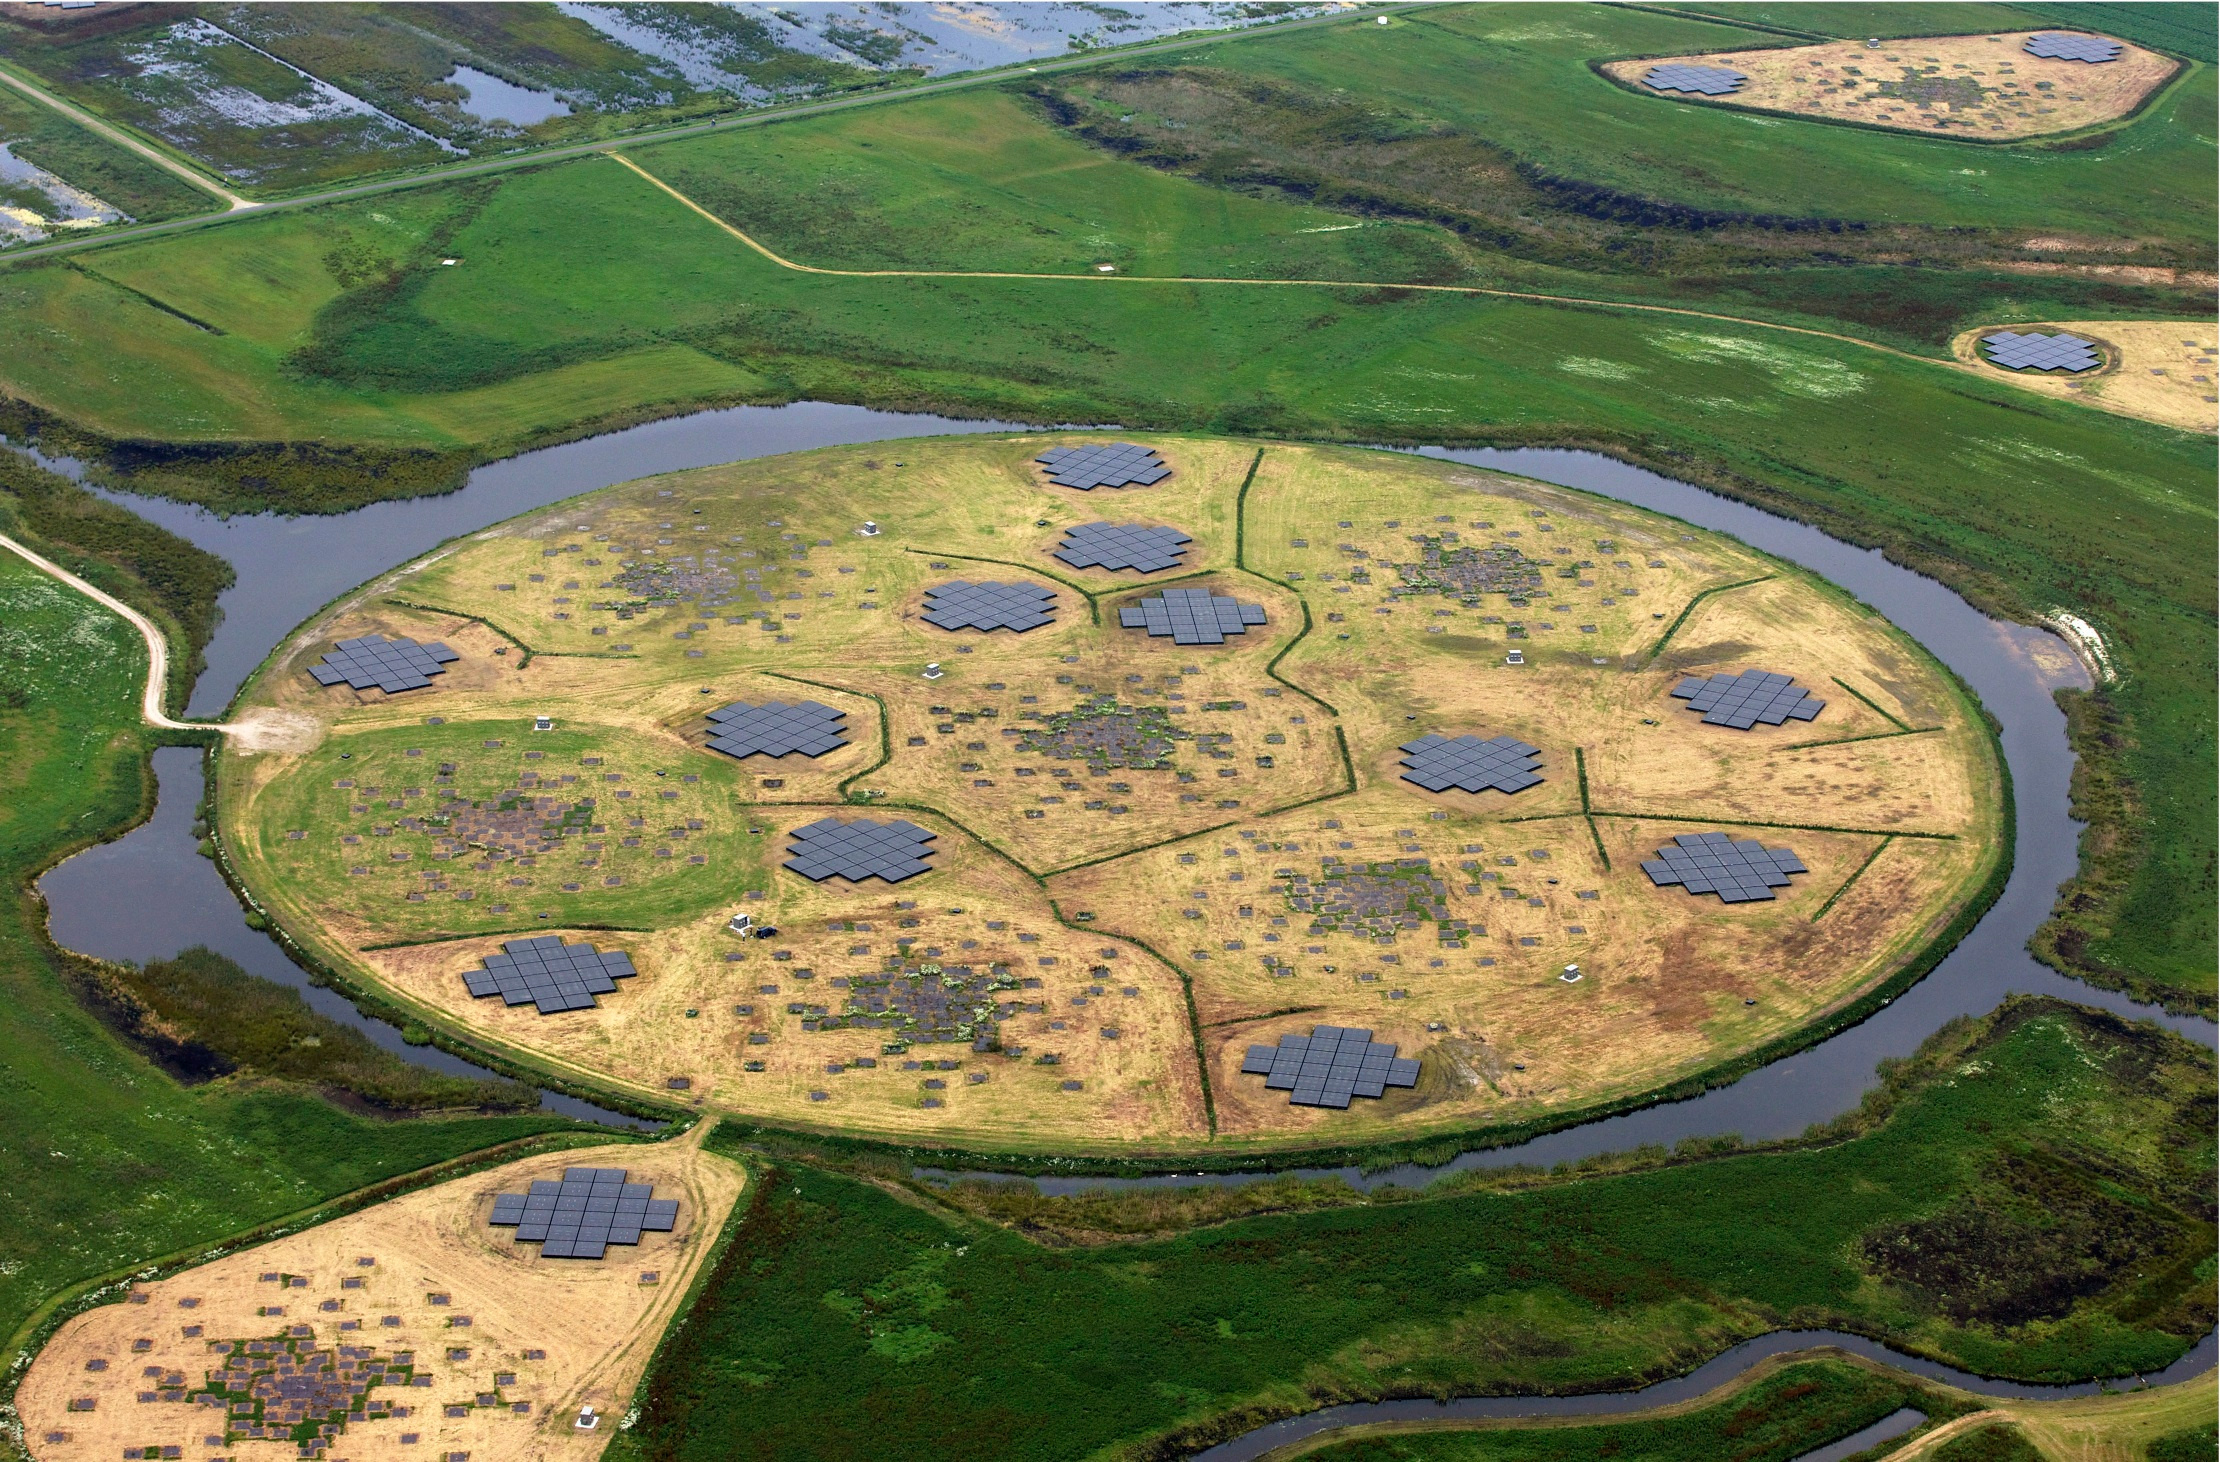
\includegraphics[width=0.8\textwidth]{LOFAR-superterp}
  \bicaption[LOFAR 核心区域的中心]{%
    \acs{lofar} 核心区域的中心.
    小块深色区域为 LBA,大块深色区域为 HBA.
  }{%
    The heart of the \acs{lofar} core.
    The small dark regions are installed with LBA,
    while the big dark regions are installed with HBA.
    \\\textcopyright{}
    \citeay{vanHaarlem2013}.
  }
  \label{fig:lofar}
\end{figure}

%---------------------------------------------------------------------
\subsection{MWA}

\acf{mwa} 位于澳大利亚西部的 Murchison 射电天文台,是 SKA1-Low 的先驱
\cite{lonsdale2009,bowman2013,tingay2013,wayth2018}.
该阵列的主要科学目标包括宇宙再电离信号探测、河内及河外射电源、暂现源和空间气候.
\acs{mwa} 工作在 \SIrange{80}{300}{\MHz} 频段,使用一种双极化偶极子天线,
每个站点包含 16 个天线(按 4 行 4 列规则排列).
所有天线均固定指向天顶,工作时通过调控各天线的时延来控制波束的合成与指向.
\acs{mwa} 自 2007 年开始建设,于 2012 年完成了一期 128 个站点的建设,
于 2017 年底完成了二期 128 个新站点的扩建工作\cite{wayth2018},目前已投入使用.
\autoref{fig:mwa} 显示了 \acs{mwa} 东侧六边形区域内的站点.
\acs{mwa} 的站点分为两部分:
一部分紧凑地排列在六边形区域内,主要用于探测再电离信号以及研究银河系大尺度结构;
另一部分散布于四周较大区域,实现较高的空间分辨率,便于开展河外射电源等研究.
\acs{mwa} 一期已完成了 \ac{gleam} 巡天项目 \cite{wayth2015},
并已发布一批成果,比如点源目录 \cite{hurleyWalker2017}、
银河系内 \Hii/ 区目录 \cite{su2018}、
高分辨率 EoR 前景模型 \cite{procopio2017}、等等.
使用 \acs{mwa} 二期开展的 \ac{gleam-x} 巡天也正在积极进行 \cite{hurleyWalker2017prop}.
作为少有的覆盖南天的低频射电巡天,\acs{gleam} 和 \acs{gleam-x}
将为 SKA1-Low 的巡天工作提供校准指导和星表的交叉认证.
同时 \acs{mwa} 也将会为 SKA1-Low 的宇宙再电离探测任务提供
更精准的天空模型和天区指导.

\begin{figure}[htp]
  \centering
  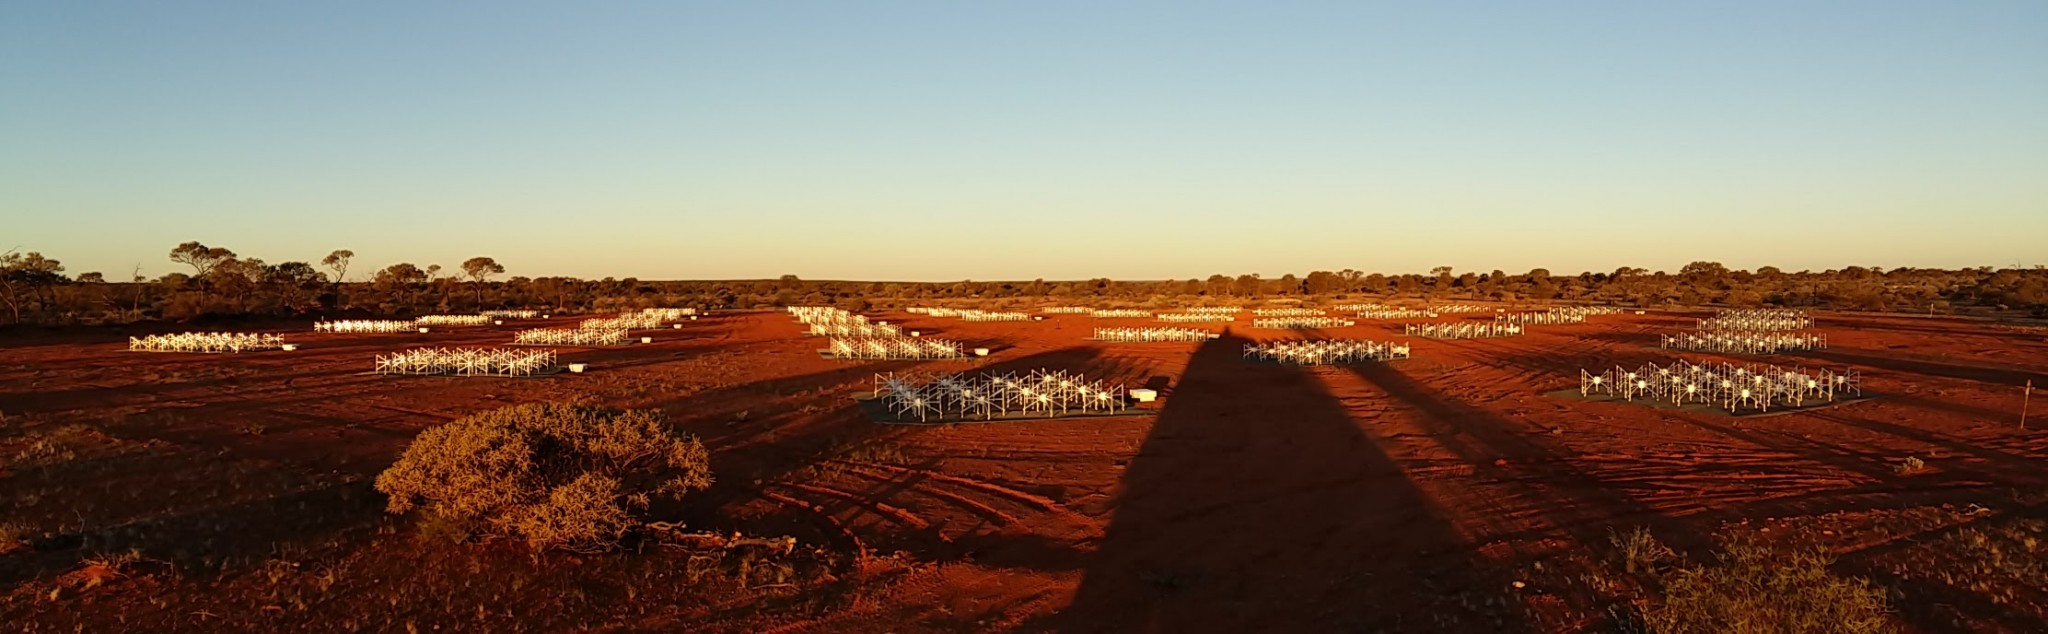
\includegraphics[width=\textwidth]{MWA}
  \bicaption[MWA 东部站点]{%
    \acs{mwa} 东侧六边形区域内的站点,每个站点包含 16 个天线.
  }{%
    The stations inside the \acs{mwa}'s east hexagonal region,
    with each station consisting of 16 antennas.
    \\\textcopyright{}
    \ac{icrar}/\acs{mwa},
    \url{https://www.icrar.org/multimedia/images/}, (2018-10-04).
  }
  \label{fig:mwa}
\end{figure}

%---------------------------------------------------------------------
\subsection{LWA}

\acf{lwa} 是一个正在建设于美国新墨西哥州中部的大型低频干涉阵列,
计划由 53 个分布远达 \SI{400}{\km} 的站点组成,
每个站点的大小约 \SI{100x100}{\meter} 并且包含 256 个双极化天线,
总接收面积达 \SI{1}{\km\squared}(在 \SI{10}{\MHz} 处),
工作在非常低频的 \SIrange{10}{88}{\MHz} 波段,
这是我们目前了解最少的射电波段 \cite{ellingson2009}.
借助其高灵敏度和高角分辨率,\acs{lwa} 将打开这一个新射电窗口,
研究宇宙高能粒子加速机制、早期宇宙及其演化、暂现源、银河系星际介质、
太阳活动及电离层性质等.
\acs{lwa} 所采用的大站点设计使其更适合研究银河系的大尺度结构.
\acs{lwa} 的首个站点(LWA1;\autoref{fig:lwa})位于\ac{vla} 附近,
已于 2009 年建设完成,并于 2011 年开始正式观测 \cite{taylor2012,ellingson2013};
其他站点正在积极建设之中.
\acs{lwa} 亦采用数字波束合成技术,但其创新之处在于每个站点均可独立使用并成像.
目前已使用 \acs{lwa}1 开展巡天并获得了 \SIrange{35}{80}{\MHz}
北天图像 \cite{dowell2017}.

\begin{figure}[htp]
  \centering
  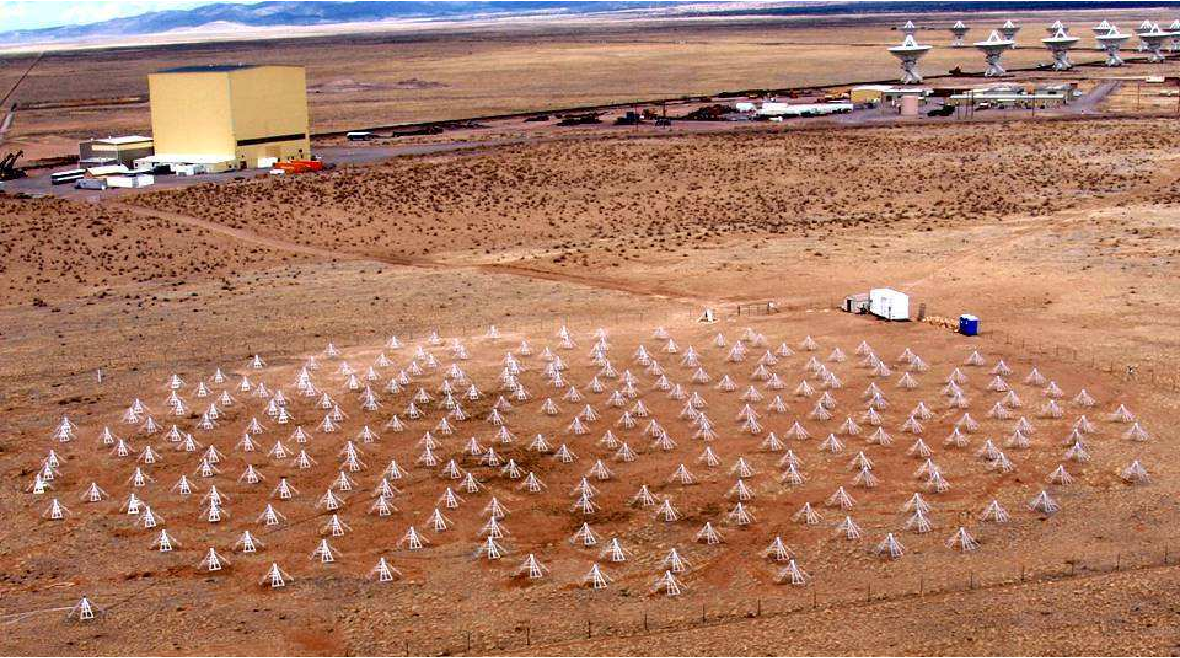
\includegraphics[width=0.8\textwidth]{LWA1}
  \bicaption[LWA 的首个站点(LWA1)]{%
    位于 \acs{vla} 附近的 \acs{lwa} 的首个站点(LWA1),包含 256 个天线.
  }{%
    The first station of \acs{lwa}, i.e., LWA1,
    which locates near the \acs{vla} and contains 256 antennas.
    \\\textcopyright{}
    \citeay{taylor2012}.
  }
  \label{fig:lwa}
\end{figure}

%---------------------------------------------------------------------
\subsection{MITEoR}
\label{ssec:miteor}

\acf{miteor} 是一个使用\ac{fftt} 新技术\cite{tegmark2009,tegmark2010}的先导阵列,
由 64 个按 8 行 8 列规则分布的全同双极化天线构成(\autoref{fig:miteor}),
在 \SIrange{100}{200}{\MHz} 范围内覆盖两个宽度为 \SI{25}{\MHz} 的频段
\cite{zheng2014}.
利用这种天线布局方式,可以直接对天线采集信号运用\ac{fft}进行成像,
避免了传统干涉阵列耗时的天线/站点间两两相关运算,
将计算复杂度由 $O(N_{\!A}^2)$ 显著降为 $O(\acs{N-ant} \log\acs{N-ant})$,
其中 \acs{N-ant} 为\acl{N-ant};
同时还将数据存储压力从 $O(N_{\!A}^2)$ 大幅减轻至 $O(\acs{N-ant})$.
如此可以极大地降低建设和运行成本,非常有利于建设超大规模的干涉阵列,
实现极高的灵敏度.
此外,阵列中的大量冗余基线能为系统自校准提供有效帮助 \cite{dillon2016}.
目前,\ac{miteor} 已开展观测并公布了 \SIrange{128}{175}{\MHz} 的北天图像
\cite{zheng2017},充分验证了 \ac{fftt} 技术的可行性.
该技术的创新性和巨大潜力能在未来 EoR 实验中发挥重要作用.

\begin{figure}[htp]
  \centering
  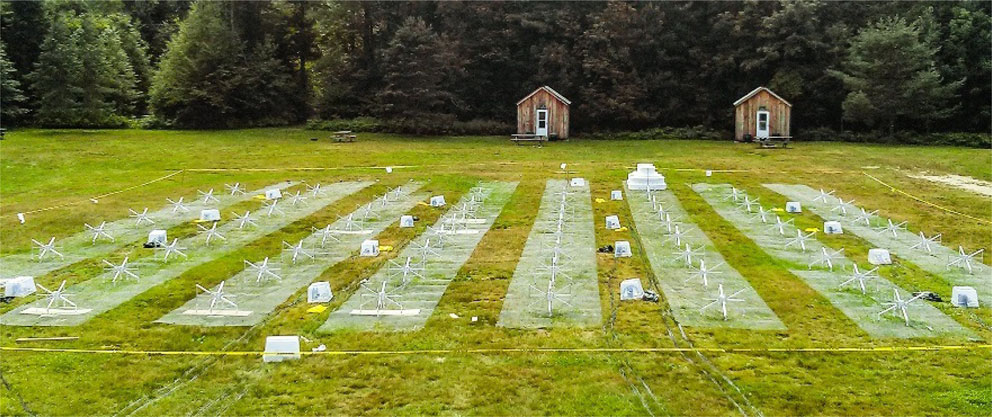
\includegraphics[width=\textwidth]{MITEoR}
  \bicaption[MITEoR 干涉阵列]{%
    在 2013 年夏天部署完成的 \acs{miteor} 干涉阵列,
    64 个双极化天线规则地分布在 \SI{21x21}{\meter} 的矩形区域,
    相互之间分隔 \SI{3}{\meter}.
  }{%
    The \acs{miteor} array deployed in the summer of 2013.
    The 64 dual-polarization antennas were laid on a \SI{21x21}{\meter}
    regular grid with a separation of \SI{3}{\meter}.
    \\\textcopyright{}
    \citeay{zheng2014}.
  }
  \label{fig:miteor}
\end{figure}

%---------------------------------------------------------------------
\subsection{HERA}

\acf{hera} 是正在南非 Karoo 射电天文保护区建造的、
继 \ac{paper} 等探路者阵列之后的第二代宇宙再电离时期探测阵列 \cite{deboer2017}.
其首要科学目标是精确测量源自宇宙再电离时期甚至\ac{cd}时期的 21\,cm 信号
及其功率谱的演化,从而描绘宇宙再电离时期以及之前的宇宙大尺度结构.
该阵列将由 350 面直径为 \SI{14}{\meter} 的固定式抛物面碟形天线构成,
观测频率为 \SIrange{50}{250}{\MHz}.
\acs{hera} 的阵型和天线设计保证了它能够为 EoR 信号的观测提供高灵敏度、
波束形状和其他仪器效应相对简单可控、
易于借助大量冗余基线对系统进行高精度校准 \cite{dillon2016}.
该设计还保证 \acs{hera} 能够有效利用\ac{delay-spec} 技术\cite{parsons2012}
和\ac{fgavd}方法(详见 \autoref{sec:fgavd})来处理观测数据.
目前 \acs{hera} 的第一期 37 面天线已经安装完毕并开始试观测
(\autoref{fig:hera} 显示了 \acs{hera} 已于 2016 年建成的 19 面天线),
第二期的 128 面天线也已开始建设,是 SKA1-Low 的有力竞争者.

\begin{figure}[htp]
  \centering
  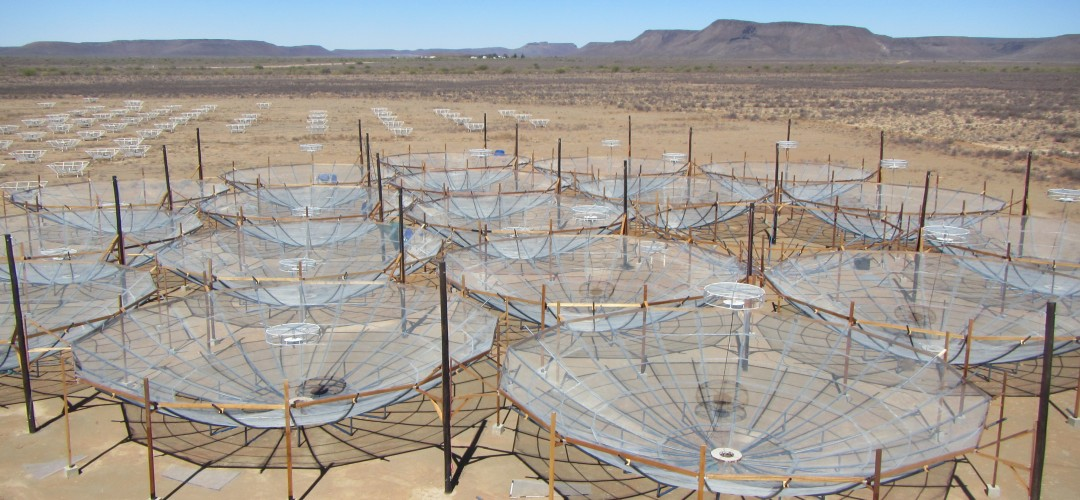
\includegraphics[width=\textwidth]{HERA19}
  \bicaption[HERA 已建成的 19 面天线]{%
    \acs{hera} 在 2016 年建成的 19 面碟形天线.
    后方的小型天线属于 \acs{paper} 项目.
  }{%
    The \acs{hera}'s 19 dish antennas deployed in South Africa in 2016.
    The small antennas in the background belong to the \acs{paper}
    experiment.
    \\\textcopyright{}
    \acs{hera}/SKA Africa, \url{http://reionization.org/}, (2018-10-04).
  }
  \label{fig:hera}
\end{figure}

%---------------------------------------------------------------------
\subsection{SKA}

\acf{ska} 是由澳大利亚、加拿大、中国、印度、意大利、新西兰、南非、瑞典、荷兰
以及英国共同参与建设的下一代巨型射电望远镜阵列,
由位于澳大利亚西部 Muchison 的低频阵列 (SKA-Low)
和位于南非 Karoo 的中频阵列 (SKA-Mid) 组成(\autoref{fig:ska}),
计划最终包含上百万个低频天线和上千面中频碟形天线,
达到约 \SI{1}{\km\squared} 的接收面积,
实现极高的灵敏度、分辨率和巡天速度.
SKA 的建设分别两期,第一期 (SKA1) 将建设约 \SI{10}{\percent} 的天线.
SKA1-Low 将由分布在 512 个站点的约 13 万根天线组成,最长基线约 \SI{65}{\km},
观测频率为 \SIrange{50}{350}{\MHz};
SKA1-Mid 将由 197 面(包含 MeerKAT 的 64 面)碟形天线组成,
最长基线约 \SI{150}{\km},观测频率为 \SI{350}{\MHz} 至 \SI{15.3}{\GHz}.
SKA 的关键科学目标有\cite{braun2015}:
宇宙再电离时期和黎明时期(功率谱测量甚至直接成像观测)\cite{mellema2013,mellema2015,koopmans2015}、
宇宙学和暗能量\cite{maartens2015,santos2015}、
脉冲星和黑洞\cite{kramer2015}、
星系形成与演化(连续谱巡天和中性氢巡天)\cite{prandoni2015,staveley2015}、
暂现源\cite{fender2015}、
宇宙磁场的起源与演化\cite{johnston2015}、
以及地外生命\cite{hoare2015}.
目前 SKA1 已在积极建设之中,预计 2025 年左右能够使用部分天线开展科学观测.

\begin{figure}[htp]
  \centering
  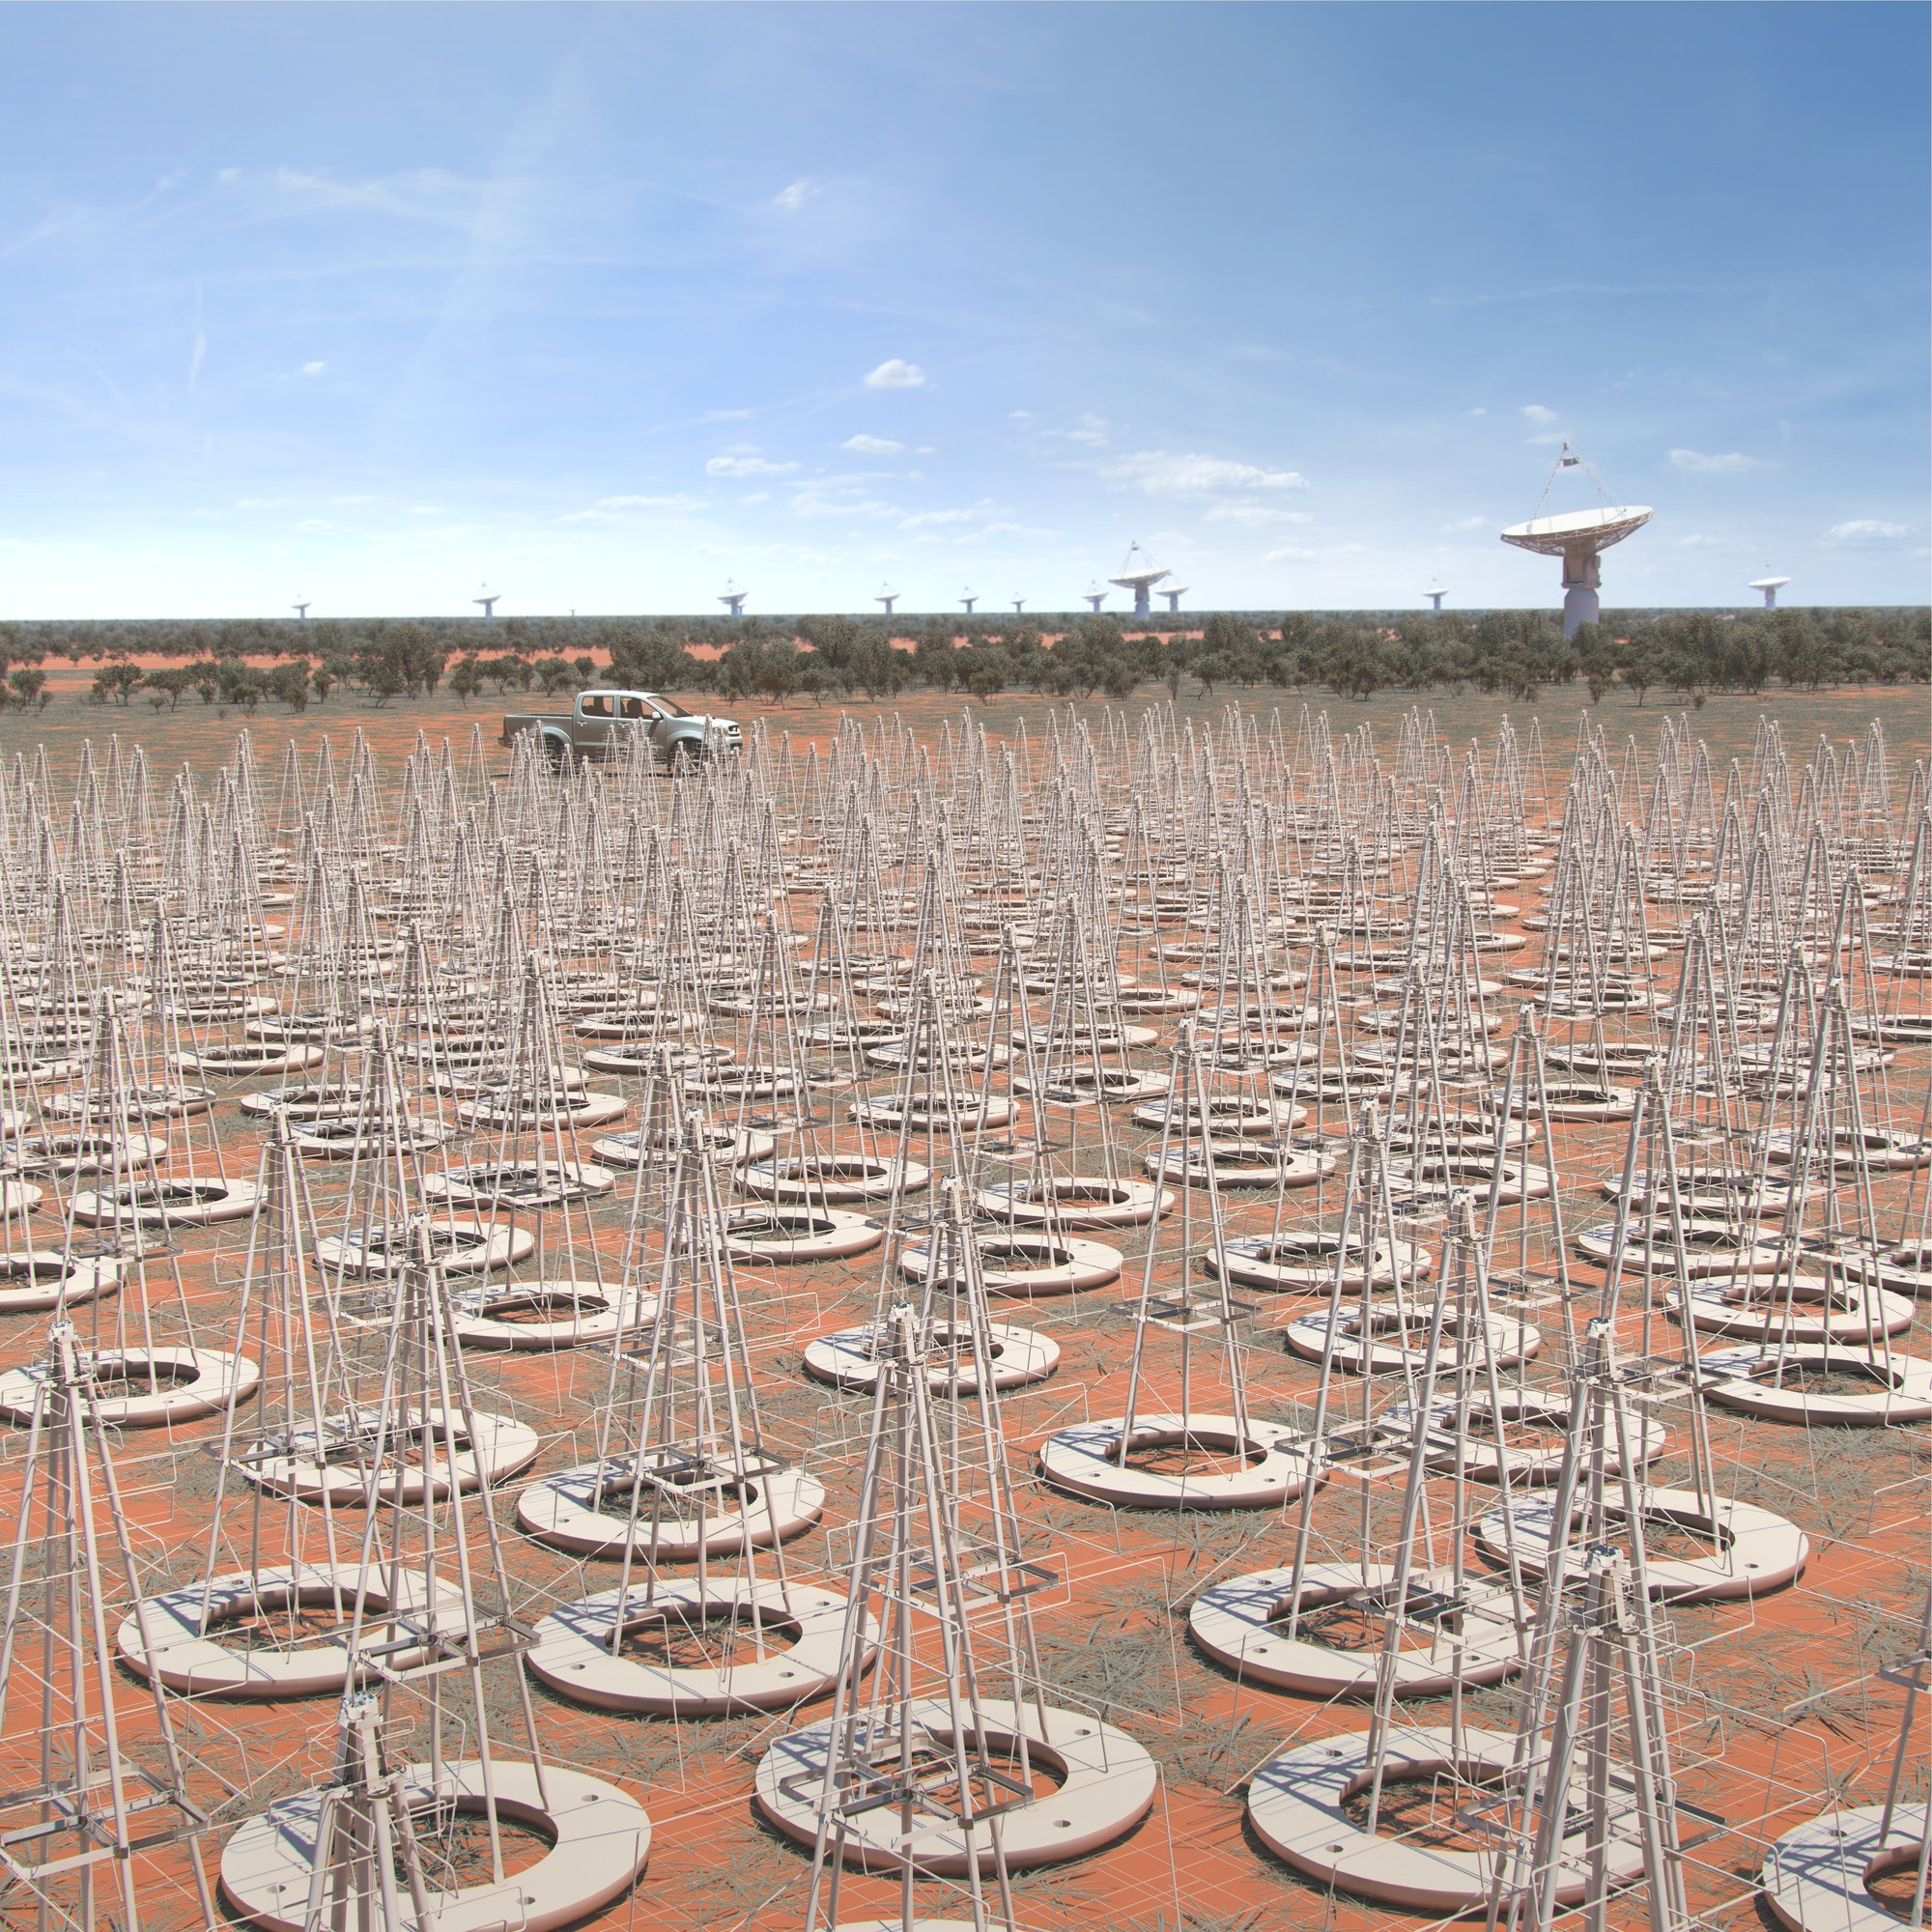
\includegraphics[width=0.5\textwidth]{SKA1-low-closeup}%
  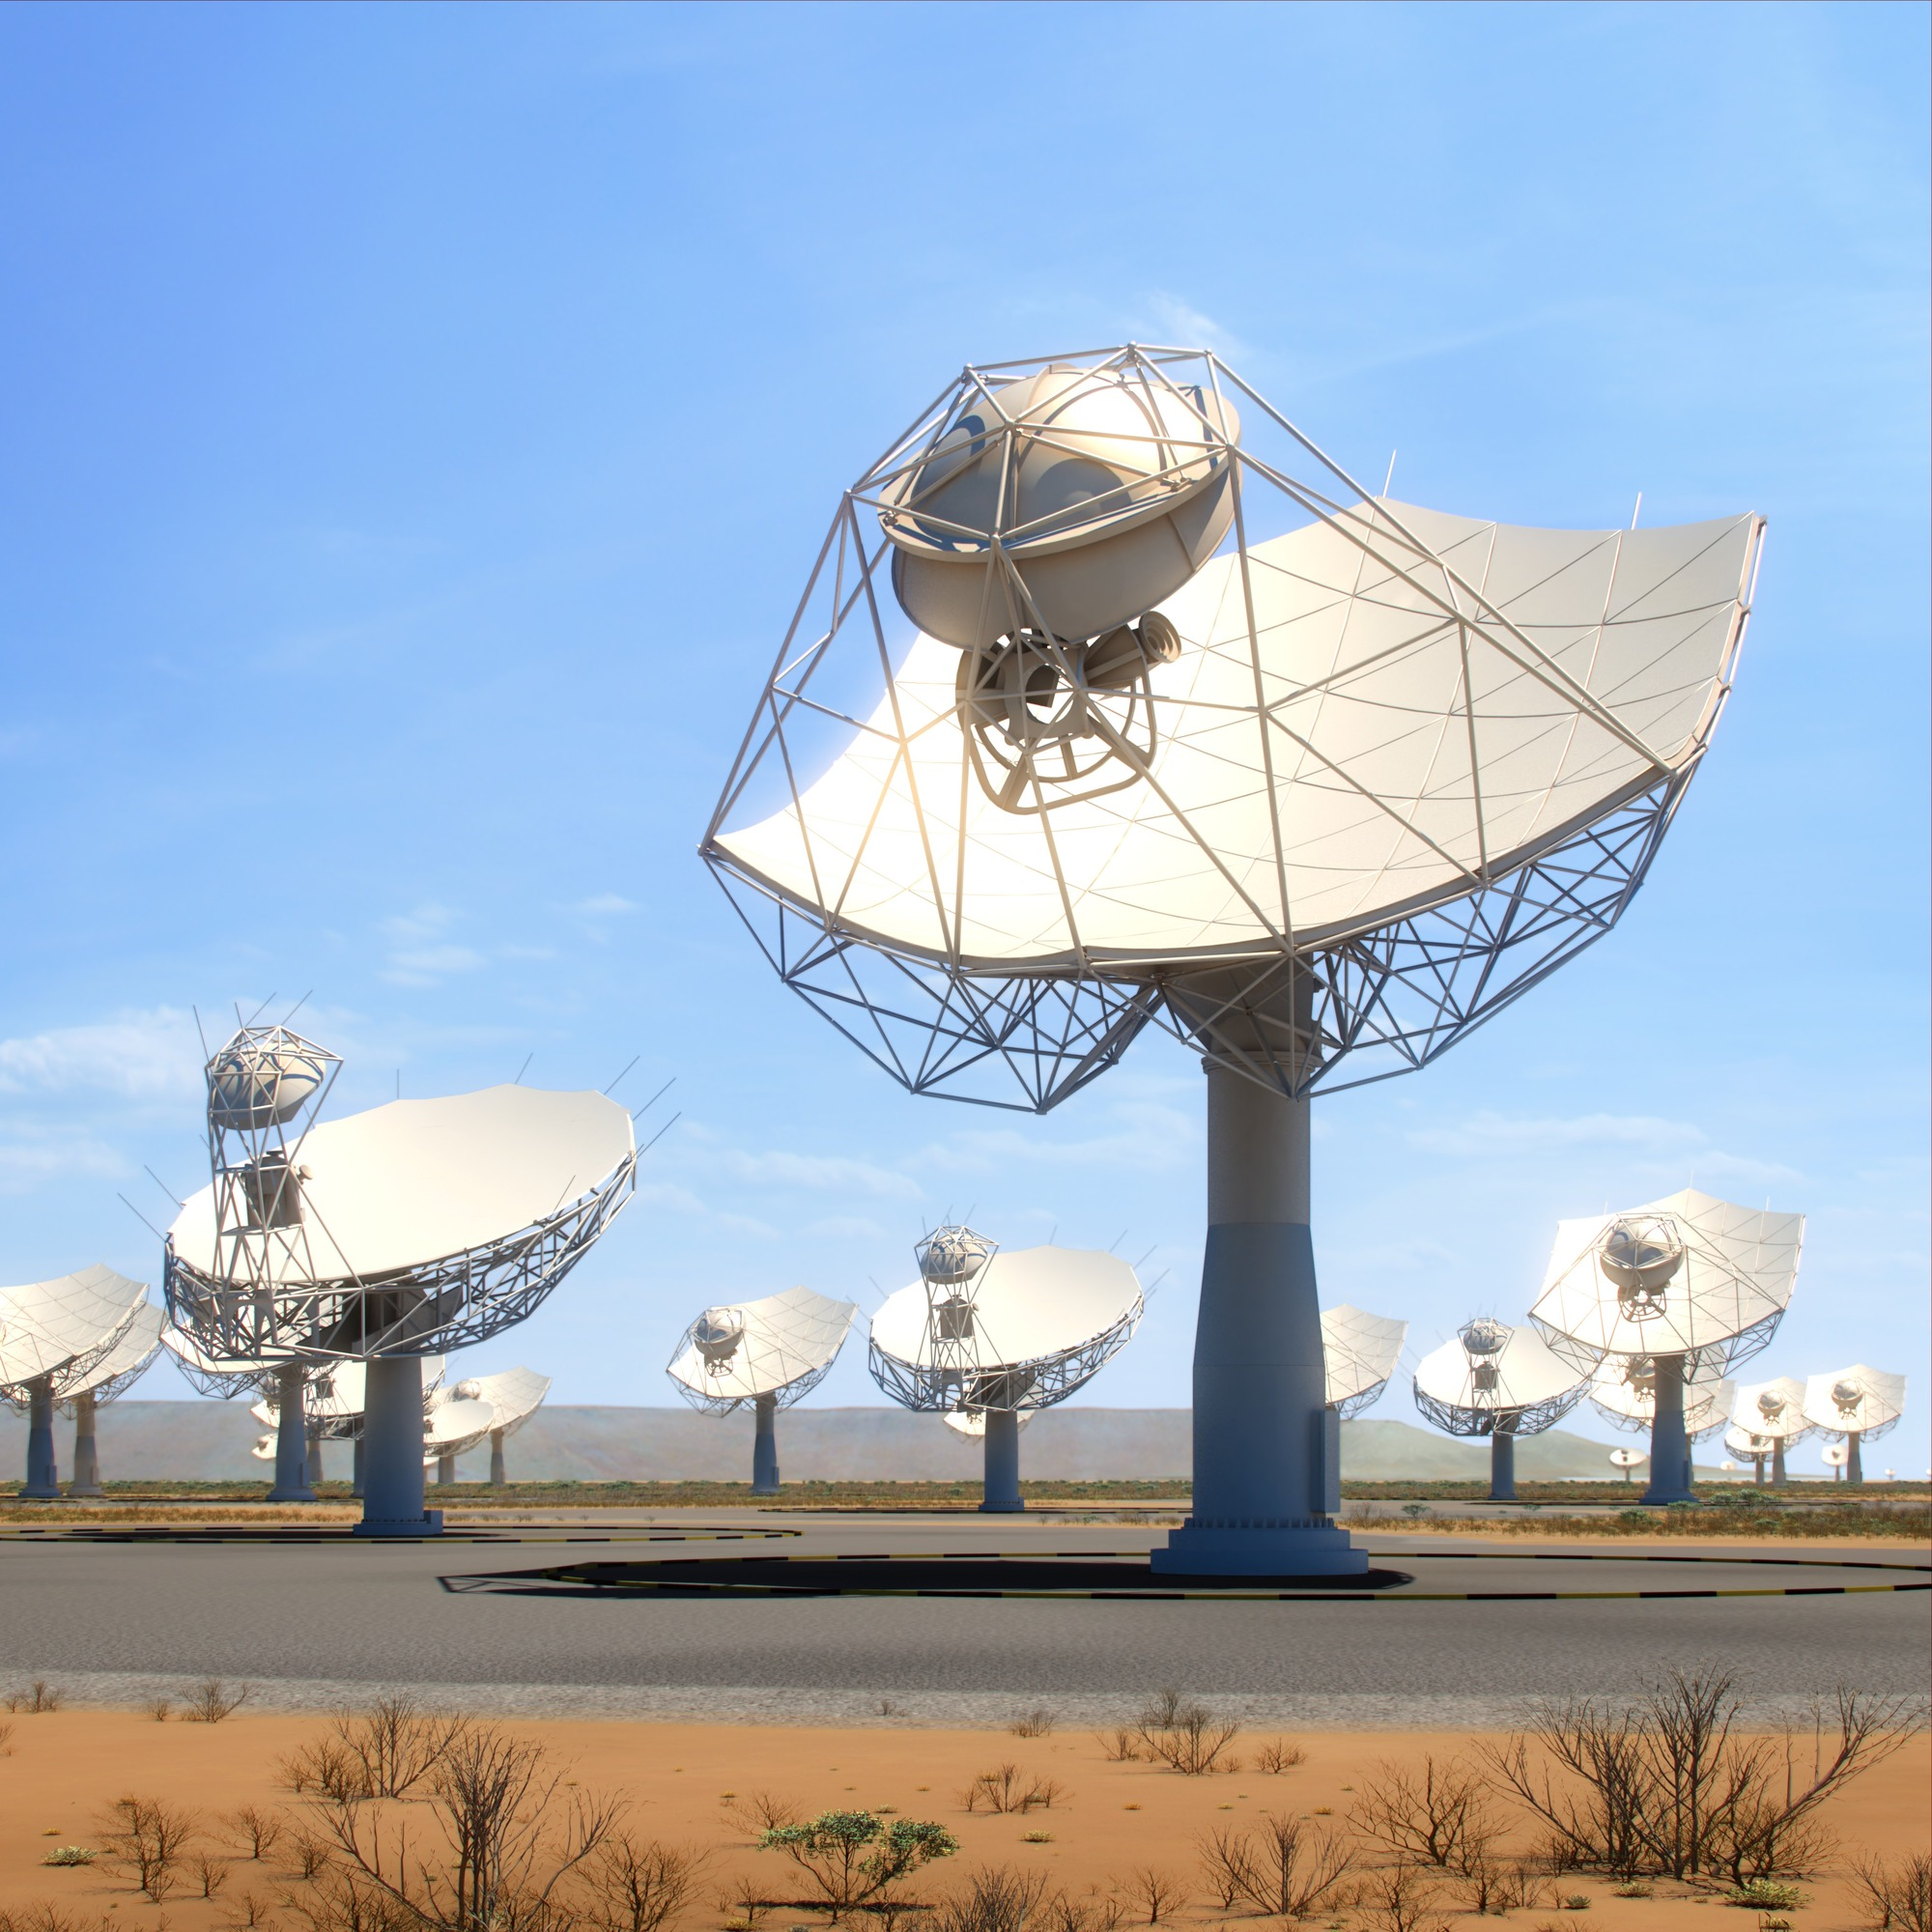
\includegraphics[width=0.5\textwidth]{SKA1-mid-closeup}
  \bicaption[SKA 低频和中频天线示意图]{%
    SKA-Low 偶极天线(左栏)和 SKA-Mid 碟形天线(右栏)的想像图.
  }{%
    The artist rendition of the SKA-Low dipole antennas (left)
    and the SKA-Mid dishes (right).
    \\\textcopyright{}
    SKA Organisation, \url{https://www.skatelescope.org/multimedia/image/}, (2019-03-17).
  }
  \label{fig:ska}
\end{figure}


%=====================================================================
\section{小结}

TODO

本章主要参考了下述资料:
\citeay{condon2016}, \citeay{clark1999}, \citeay{thompson1999},
\citeay{thompson2017}, \citeay{wilson2014}.

%% EOF
